% !TeX program = xelatex
% Template báo cáo bài tập lớn học phần Nhập môn Học máy (FIT4013) - Đại học Đại Nam
% Đề tài 3: Phân loại tin nhắn rác (SMS Spam Collection)
% Nhóm thực hiện: Nhóm 13 (Nguyễn Hoàng Hải, Nguyễn Thành Đạt)

\documentclass[12pt,a4paper,oneside]{extreport}

% Nạp cấu hình chung
% =====================================================
% settings.tex
% Cấu hình chung cho báo cáo Bài tập lớn Học máy FIT4013
% =====================================================

% =========================
% 1. CẤU HÌNH TIẾNG VIỆT VÀ FONT
% =========================
\usepackage{fontspec}
\IfFontExistsTF{Times New Roman}
  {\setmainfont{Times New Roman}}
  {\setmainfont{Tinos}}

\usepackage{polyglossia}
\setdefaultlanguage{vietnamese}

% =========================
% 2. CẤU HÌNH TRANG
% =========================
\usepackage[
    a4paper,
    left=3.0cm,
    right=1.5cm,
    top=2.0cm,
    bottom=2.0cm
]{geometry}

\usepackage{setspace}
\onehalfspacing

% Cỡ chữ mặc định của nội dung là 13pt.
\makeatletter
\renewcommand{\normalsize}{%
    \@setfontsize\normalsize{13pt}{15.6pt}%
    \abovedisplayskip 13pt plus 3pt minus 7pt%
    \abovedisplayshortskip 0pt plus 4pt%
    \belowdisplayshortskip 6.5pt plus 3.5pt minus 3pt%
    \belowdisplayskip \abovedisplayskip
    \let\@listi\@listI
}
\makeatother
\normalsize

\usepackage{indentfirst}
\setlength{\parindent}{1.27cm}
\setlength{\parskip}{6pt}

% =========================
% 3. GÓI HỖ TRỢ
% =========================
\usepackage{graphicx}
\usepackage{float}
\usepackage{array}
\usepackage{longtable}
\usepackage{booktabs}
\usepackage{multirow}
\usepackage{tabularx}
\usepackage{caption}
\usepackage{amsmath, amssymb}
\usepackage{enumitem}
\setlist[itemize]{
    label=-,
    leftmargin=1.27cm,
    labelsep=0.5em
}
\usepackage{titlesec}
\usepackage{tocloft}
\usepackage{hyperref}
\usepackage{tikz}
\usetikzlibrary{arrows.meta,positioning,shapes.geometric,fit,backgrounds,calc}
\usepackage{eso-pic}
\usepackage{fancyhdr}
\usepackage{xcolor}
\usepackage{listings}

% Cấu hình listings cho mã nguồn Python
\definecolor{codegreen}{rgb}{0,0.5,0}
\definecolor{codegray}{rgb}{0.5,0.5,0.5}
\definecolor{codepurple}{rgb}{0.58,0,0.82}
\definecolor{backcolour}{rgb}{0.97,0.97,0.97}

\lstdefinestyle{mystyle}{
    backgroundcolor=\color{backcolour},   
    commentstyle=\color{codegreen}\itshape,
    keywordstyle=\color{blue}\bfseries,
    numberstyle=\tiny\color{codegray},
    stringstyle=\color{codepurple},
    basicstyle=\ttfamily\footnotesize,
    breakatwhitespace=false,         
    breaklines=true,                 
    captionpos=b,                    
    keepspaces=true,                 
    numbers=left,                    
    numbersep=5pt,                  
    showspaces=false,                
    showstringspaces=false,
    showtabs=false,                  
    tabsize=2,
    frame=single,
    rulecolor=\color{codegray!40}
}
\lstset{style=mystyle}

% =========================
% 4. HYPERLINK
% =========================
\hypersetup{
    colorlinks=true,
    linkcolor=black,
    citecolor=black,
    urlcolor=blue
}

% Số trang đặt giữa phía trên; áp dụng cả cho trang mở đầu chương.
\setlength{\headheight}{17pt}
\pagestyle{fancy}
\fancyhf{}
\fancyhead[C]{\thepage}
\renewcommand{\headrulewidth}{0pt}
\fancypagestyle{plain}{
    \fancyhf{}
    \fancyhead[C]{\thepage}
    \renewcommand{\headrulewidth}{0pt}
}

% =========================
% 5. ĐÁNH SỐ HÌNH, BẢNG THEO CHƯƠNG
% =========================
\counterwithin{table}{chapter}
\counterwithin{figure}{chapter}
\renewcommand{\thetable}{\thechapter.\arabic{table}}
\renewcommand{\thefigure}{\thechapter.\arabic{figure}}

% Môi trường riêng cho sơ đồ để đánh số và lập danh mục độc lập.
\newfloat{sodo}{H}{los}[chapter]
\floatname{sodo}{Sơ đồ}
\renewcommand{\thesodo}{\thechapter.\arabic{sodo}}
\makeatletter
\newcommand{\l@sodo}[2]{%
    \begingroup
    \let\ReportOriginalNumberline\numberline
    \renewcommand{\numberline}[1]{%
        \ReportOriginalNumberline{Sơ đồ~##1}}%
    \@dottedtocline{1}{0pt}{2.8cm}{#1}{#2}%
    \endgroup
}
\makeatother

\captionsetup{
    font=normalsize,
    labelfont=normalfont,
    textfont=normalfont,
    labelsep=period,
    justification=centering
}
\captionsetup[table]{name=Bảng,position=top}
\captionsetup[figure]{name=Hình,position=bottom}
\captionsetup[sodo]{name=Sơ đồ,position=bottom}

\renewcommand{\listtablename}{BẢNG}
\renewcommand{\listfigurename}{HÌNH, SƠ ĐỒ}
\renewcommand{\contentsname}{MỤC LỤC}
\renewcommand{\bibname}{TÀI LIỆU THAM KHẢO}

% =========================
% 6. ĐỊNH DẠNG TIÊU ĐỀ CHƯƠNG, MỤC
% =========================
\titleformat{\chapter}
  [display]
  {\centering\bfseries\fontsize{14pt}{16pt}\selectfont}
  {Chương \thechapter}
  {0.3cm}
  {\MakeUppercase}

\titlespacing*{\chapter}{0pt}{0pt}{18pt}

\titleformat{\section}
  {\bfseries\fontsize{13pt}{15pt}\selectfont}
  {\thesection}
  {0.5em}
  {}

\titleformat{\subsection}
  {\bfseries\itshape\fontsize{13pt}{15pt}\selectfont}
  {\thesubsection}
  {0.5em}
  {}

\titleformat{\subsubsection}
  {\itshape\fontsize{13pt}{15pt}\selectfont}
  {\thesubsubsection}
  {0.5em}
  {}

\setcounter{secnumdepth}{3}
\setcounter{tocdepth}{3}

% =========================
% 7. ĐỊNH DẠNG MỤC LỤC
% =========================
\renewcommand{\cftchapfont}{\bfseries\fontsize{12pt}{14pt}\selectfont}
\renewcommand{\cftchappagefont}{\bfseries\fontsize{12pt}{14pt}\selectfont}
\renewcommand{\cftchappresnum}{CHƯƠNG~}
\renewcommand{\cftchapaftersnum}{.}
\setlength{\cftchapnumwidth}{2.5cm}
\renewcommand{\cftsecfont}{\bfseries\fontsize{12pt}{14pt}\selectfont}
\renewcommand{\cftsecpagefont}{\bfseries\fontsize{12pt}{14pt}\selectfont}
\renewcommand{\cftsecaftersnum}{.}
\renewcommand{\cftsubsecfont}{\itshape\fontsize{12pt}{14pt}\selectfont}
\renewcommand{\cftsubsecpagefont}{\fontsize{12pt}{14pt}\selectfont}
\renewcommand{\cftsubsecaftersnum}{.}
\renewcommand{\cftsubsubsecfont}{\fontsize{12pt}{14pt}\selectfont}
\renewcommand{\cftsubsubsecpagefont}{\fontsize{12pt}{14pt}\selectfont}
\renewcommand{\cftsubsubsecaftersnum}{.}
\renewcommand{\cftchapleader}{\cftdotfill{\cftdotsep}}
\setlength{\cftbeforechapskip}{6pt}

\renewcommand{\cfttoctitlefont}{\hfill\bfseries\fontsize{14pt}{16pt}\selectfont}
\renewcommand{\cftaftertoctitle}{\hfill}
\setlength{\cftbeforetoctitleskip}{0pt}
\setlength{\cftaftertoctitleskip}{18pt}

\makeatletter
\newcommand{\ReportListTable}[4]{%
    {\bfseries\fontsize{13pt}{14pt}\selectfont #1:\par}
    \vspace{6pt}
    \begingroup
    \fontsize{12pt}{13pt}\selectfont
    \renewcommand{\arraystretch}{1.5}
    \def\ReportListPrefix{#3}%
    \def\numberline##1{\ReportListPrefix~##1.\enspace}%
    \def\contentsline##1##2##3##4{##2\dotfill & ##3\\\hline}%
    \def\addvspace##1{}%
    \def\select@language##1{}%
    \makeatletter
    \noindent
    \begin{tabular}{|>{\raggedright\arraybackslash}p{\dimexpr\textwidth-3.5cm\relax}|>{\centering\arraybackslash}p{2.6cm}|}
        \hline
        \multicolumn{1}{|c|}{\bfseries #2} & \bfseries Trang \\
        \hline
        \@input{\jobname.#4}%
    \end{tabular}
    \par
    \let\contentsline\@gobblefour
    \let\addvspace\@gobble
    \let\select@language\@gobble
    \@starttoc{#4}%
    \makeatother
    \endgroup
}

\newcommand{\CombinedLists}{%
    \chapter*{\fontsize{13pt}{14pt}\selectfont DANH MỤC CÁC BẢNG, SƠ ĐỒ, HÌNH}
    \addcontentsline{toc}{chapter}{DANH MỤC CÁC BẢNG, SƠ ĐỒ, HÌNH}
    \ReportListTable{BẢNG}{Tên bảng}{Bảng}{lot}
    \vspace{14pt}
    \ReportListTable{SƠ ĐỒ}{Tên sơ đồ}{Sơ đồ}{los}
    \vspace{14pt}
    \ReportListTable{HÌNH}{Tên hình}{Hình}{lof}
}
\makeatother

% =========================
% 8. THÔNG TIN SINH VIÊN / BÁO CÁO
% =========================
\newcommand{\BoGiaoDuc}{BỘ GIÁO DỤC VÀ ĐÀO TẠO}
\newcommand{\TenTruong}{TRƯỜNG ĐẠI HỌC ĐẠI NAM}
\newcommand{\Khoa}{KHOA CÔNG NGHỆ THÔNG TIN}

\newcommand{\TenSinhVienMot}{NGUYỄN HOÀNG HẢI}
\newcommand{\MaSinhVienMot}{1871020211}

\newcommand{\TenSinhVienHai}{NGUYỄN THÀNH ĐẠT}
\newcommand{\MaSinhVienHai}{1871020135}

\newcommand{\LopHoc}{CNTT 18-10}
\newcommand{\NhomHocTap}{NHÓM 13}
\newcommand{\HocPhan}{NHẬP MÔN HỌC MÁY (MÃ HP: FIT4013)}

\newcommand{\TenBaoCao}{BÁO CÁO BÀI TẬP LỚN HỌC PHẦN NHẬP MÔN HỌC MÁY\\[0.3cm]\Large\textbf{ĐỀ TÀI 3: PHÂN LOẠI TIN NHẮN RÁC (SMS SPAM COLLECTION)}\\[0.2cm]\large\textbf{NGHIÊN CỨU SO SÁNH MULTINOMIAL NAIVE BAYES, K-NN VÀ CÂY QUYẾT ĐỊNH}}
\newcommand{\LoaiBaoCao}{BÁO CÁO BÀI TẬP LỚN}
\newcommand{\Nganh}{CÔNG NGHỆ THÔNG TIN}
\newcommand{\ChuyenNganh}{KHOA HỌC DỮ LIỆU VÀ TRÍ TUỆ NHÂN TẠO}

\newcommand{\GiangVienHD}{ThS. Lê Thị Thùy Trang}

\newcommand{\DiaDiem}{HÀ NỘI}
\newcommand{\Nam}{2026}

\newcommand{\LogoTruong}{images/logo-dai-nam.png}

% =========================
% 9. LỆNH CHƯƠNG KHÔNG ĐÁNH SỐ
% =========================
\newcommand{\UnnumberedChapter}[1]{
    \chapter*{#1}
    \addcontentsline{toc}{chapter}{#1}
}

\newcommand{\Nguon}[1]{%
    \par\smallskip
    {\centering\itshape Nguồn: #1\par}
}

\newcommand{\SodoCaption}[2]{%
    \caption[#1]{#1\\[3pt]\textit{Nguồn: #2}}%
}

% =========================
% 10. KHUNG TRANG BÌA
% =========================
\newcommand{\DrawCoverBorder}{
\AddToShipoutPictureBG*{
\begin{tikzpicture}[remember picture, overlay]
    \draw[line width=1.5pt]
        ([xshift=1.2cm,yshift=-1.2cm]current page.north west)
        rectangle
        ([xshift=-1.2cm,yshift=1.2cm]current page.south east);
    \draw[line width=0.5pt]
        ([xshift=1.3cm,yshift=-1.3cm]current page.north west)
        rectangle
        ([xshift=-1.3cm,yshift=1.3cm]current page.south east);
\end{tikzpicture}
}
}

\begin{document}

% =========================
% TRANG BÌA
% =========================
\pagenumbering{gobble}
% =====================================================
% cover.tex
% Hai trang bìa theo mẫu quy chuẩn của Trường Đại học Đại Nam
% =====================================================

% =========================
% TRANG BÌA 1 (BÌA CHÍNH)
% =========================
\begin{titlepage}
\DrawCoverBorder
\centering

{\bfseries\fontsize{14pt}{17pt}\selectfont \BoGiaoDuc \par}
\vspace{0.2cm}
{\bfseries\fontsize{15pt}{18pt}\selectfont \TenTruong \par}
\vspace{0.2cm}
{\bfseries\fontsize{13pt}{16pt}\selectfont \Khoa \par}

\vspace{0.8cm}

\includegraphics[width=0.25\textwidth]{\LogoTruong}

\vspace{0.8cm}

{\bfseries\fontsize{18pt}{22pt}\selectfont \LoaiBaoCao \par}
\vspace{0.3cm}
{\bfseries\fontsize{13pt}{16pt}\selectfont HỌC PHẦN: \HocPhan \par}

\vspace{1.0cm}

{\bfseries\fontsize{16pt}{20pt}\selectfont ĐỀ TÀI 3: PHÂN LOẠI TIN NHẮN RÁC\\[0.2cm](SMS SPAM COLLECTION) \par}
\vspace{0.4cm}
{\bfseries\fontsize{13pt}{16pt}\selectfont NGHIÊN CỨU SO SÁNH MULTINOMIAL NAIVE BAYES,\\[0.1cm]K-NN VÀ CÂY QUYẾT ĐỊNH \par}

\vspace{1.5cm}

\begin{table}[H]
\centering
\fontsize{13pt}{16pt}\selectfont
\begin{tabular}{rll}
\textbf{Nhóm học tập:} & \multicolumn{2}{l}{\textbf{\NhomHocTap}} \\
\textbf{Sinh viên thực hiện:} & \textbf{\TenSinhVienMot} & \textbf{MSV: \MaSinhVienMot} \\
& \textbf{\TenSinhVienHai} & \textbf{MSV: \MaSinhVienHai} \\
\textbf{Lớp:} & \multicolumn{2}{l}{\textbf{\LopHoc}} \\
\textbf{Ngành:} & \multicolumn{2}{l}{\textbf{\Nganh}} \\
\textbf{Giảng viên hướng dẫn:} & \multicolumn{2}{l}{\textbf{\GiangVienHD}} \\
\end{tabular}
\end{table}

\vfill

{\bfseries\fontsize{13pt}{16pt}\selectfont \DiaDiem, NĂM \Nam \par}

\end{titlepage}

% =========================
% TRANG BÌA 2 (BÌA PHỤ)
% =========================
\begin{titlepage}
\DrawCoverBorder
\centering

{\bfseries\fontsize{14pt}{17pt}\selectfont \BoGiaoDuc \par}
\vspace{0.2cm}
{\bfseries\fontsize{15pt}{18pt}\selectfont \TenTruong \par}
\vspace{0.2cm}
{\bfseries\fontsize{13pt}{16pt}\selectfont \Khoa \par}

\vspace{0.8cm}

\includegraphics[width=0.25\textwidth]{\LogoTruong}

\vspace{0.8cm}

{\bfseries\fontsize{18pt}{22pt}\selectfont \LoaiBaoCao \par}
\vspace{0.3cm}
{\bfseries\fontsize{13pt}{16pt}\selectfont HỌC PHẦN: \HocPhan \par}

\vspace{1.0cm}

{\bfseries\fontsize{16pt}{20pt}\selectfont ĐỀ TÀI 3: PHÂN LOẠI TIN NHẮN RÁC\\[0.2cm](SMS SPAM COLLECTION) \par}
\vspace{0.4cm}
{\bfseries\fontsize{13pt}{16pt}\selectfont NGHIÊN CỨU SO SÁNH MULTINOMIAL NAIVE BAYES,\\[0.1cm]K-NN VÀ CÂY QUYẾT ĐỊNH \par}

\vspace{1.2cm}

\begin{table}[H]
\centering
\fontsize{13pt}{16pt}\selectfont
\begin{tabular}{rll}
\textbf{Nhóm học tập:} & \multicolumn{2}{l}{\textbf{\NhomHocTap}} \\
\textbf{Sinh viên thực hiện:} & \textbf{\TenSinhVienMot} & \textbf{MSV: \MaSinhVienMot} \\
& \textbf{\TenSinhVienHai} & \textbf{MSV: \MaSinhVienHai} \\
\textbf{Lớp:} & \multicolumn{2}{l}{\textbf{\LopHoc}} \\
\textbf{Ngành:} & \multicolumn{2}{l}{\textbf{\Nganh}} \\
\textbf{Chuyên ngành:} & \multicolumn{2}{l}{\textbf{\ChuyenNganh}} \\
\textbf{Giảng viên hướng dẫn:} & \multicolumn{2}{l}{\textbf{\GiangVienHD}} \\
\end{tabular}
\end{table}

\vfill

{\bfseries\fontsize{13pt}{16pt}\selectfont \DiaDiem, NĂM \Nam \par}

\end{titlepage}

% =========================
% PHẦN ĐẦU BÁO CÁO
% =========================
\clearpage
\pagenumbering{roman}
\setcounter{page}{1}

\UnnumberedChapter{LỜI CAM ĐOAN}

Chúng em xin cam đoan rằng Báo cáo bài tập lớn học phần Nhập môn Học máy (mã học phần: FIT4013) với Đề tài 3: \textit{“Phân loại tin nhắn rác (SMS Spam Collection) – Nghiên cứu so sánh các thuật toán Multinomial Naive Bayes, K-NN và Cây quyết định”} là công trình nghiên cứu, khảo sát thực nghiệm và xây dựng giải pháp của tập thể Nhóm 13 dưới sự hướng dẫn trực tiếp của giảng viên ThS. Lê Thị Thùy Trang.

Mọi số liệu thực nghiệm, bảng biểu, đồ thị phân tích, ma trận nhầm lẫn và mã nguồn chương trình được trình bày trong báo cáo này đều được thu thập và thực thi một cách trung thực, minh bạch từ bộ dữ liệu thực tế SMS Spam Collection của kho lưu trữ UCI Machine Learning Repository. Các đoạn mã nguồn tham khảo, các gói thư viện mã nguồn mở và những tài liệu khoa học được sử dụng đều có trích dẫn nguồn gốc xuất xứ rõ ràng theo đúng chuẩn mực học thuật.

Chúng em xin hoàn toàn chịu trách nhiệm trước Khoa Công nghệ Thông tin và Trường Đại học Đại Nam về tính trung thực, chuẩn xác của toàn bộ nội dung được trình bày trong bản báo cáo này.

\vspace{1cm}

\begin{flushright}
\begin{minipage}{9cm}
\centering
\textit{Hà Nội, ngày \ldots\ldots tháng \ldots\ldots năm \Nam}

\vspace{0.4cm}

\textbf{TẬP THỂ TÁC GIẢ (NHÓM 13)}

\vspace{2.2cm}

\textbf{\TenSinhVienMot \quad --- \quad \TenSinhVienHai}
\end{minipage}
\end{flushright}
\UnnumberedChapter{LỜI CẢM ƠN}

Lời đầu tiên, tập thể Nhóm 13 chúng em xin bày tỏ lòng biết ơn sâu sắc nhất tới Ban Giám hiệu Trường Đại học Đại Nam và Ban Chủ nhiệm Khoa Công nghệ Thông tin đã tạo điều kiện học tập tốt nhất, xây dựng chương trình đào tạo hiện đại, thực tiễn và cung cấp đầy đủ cơ sở vật chất kỹ thuật giúp chúng em tiếp thu kiến thức chuyên ngành một cách hiệu quả.

Đặc biệt, chúng em xin gửi lời tri ân chân thành và sâu sắc nhất tới cô giáo hướng dẫn --- \textbf{ThS. Lê Thị Thùy Trang}. Trong suốt quá trình học tập học phần Nhập môn Học máy (FIT4013) cũng như trong suốt thời gian nhóm triển khai bài tập lớn, cô đã luôn tận tình truyền đạt những kiến thức nền tảng vững chắc, chỉ dẫn phương pháp luận nghiên cứu khoa học chuẩn mực, định hướng cách tiếp cận bài toán từ dữ liệu thực tế, đồng thời dành nhiều thời gian quý báu để góp ý chi tiết, định hướng giải pháp kỹ thuật và chỉnh sửa từng thiếu sót trong mã nguồn cũng như cấu trúc báo cáo của nhóm. Những lời chỉ bảo tận tâm của cô không chỉ giúp chúng em hoàn thành tốt bài tập lớn này mà còn là hành trang quý giá cho chúng em trên con đường học tập và nghiên cứu sau này.

Chúng em cũng xin chân thành cảm ơn các thầy cô giáo trong Khoa Công nghệ Thông tin, những người đã nhiệt tình giảng dạy các học phần cơ sở ngành và chuyên ngành, tạo nền móng tư duy logic và kỹ năng lập trình giúp chúng em có đủ năng lực giải quyết bài toán học máy này.

Mặc dù cả nhóm đã dành nhiều thời gian, tâm huyết và nỗ lực tối đa để hoàn thiện đề tài từ việc tiền xử lý dữ liệu, thiết kế pipeline, tối ưu hóa siêu tham số, phân tích định lượng đến việc biên soạn tài liệu báo cáo một cách cẩn trọng nhất, song do kiến thức và kinh nghiệm thực tiễn của sinh viên còn có những giới hạn nhất định, bản báo cáo khó tránh khỏi những điểm chưa thực sự hoàn hảo. Chúng em rất kính mong nhận được những ý kiến nhận xét, góp ý và chỉ dẫn quý báu của quý thầy cô trong Hội đồng chấm bài tập lớn để công trình của nhóm được hoàn thiện hơn nữa.

Chúng em xin kính chúc quý thầy cô luôn dồi dào sức khỏe, niềm vui và gặt hái được nhiều thành tựu rực rỡ hơn nữa trong sự nghiệp trồng người cao quý!

\vspace{1cm}

\begin{flushright}
\begin{minipage}{9cm}
\centering
\textit{Hà Nội, ngày \ldots\ldots tháng \ldots\ldots năm \Nam}

\vspace{0.4cm}

\textbf{TẬP THỂ TÁC GIẢ (NHÓM 13)}

\vspace{2.2cm}

\textbf{\TenSinhVienMot \quad --- \quad \TenSinhVienHai}
\end{minipage}
\end{flushright}
\UnnumberedChapter{KÍ HIỆU CÁC CỤM TỪ VIẾT TẮT}

\begin{table}[H]
\centering
\fontsize{12pt}{15pt}\selectfont
\begin{tabular}{|p{3.5cm}|p{11.5cm}|}
\hline
\centering\textbf{TỪ VIẾT TẮT} & \centering\arraybackslash\textbf{TÊN ĐẦY ĐỦ / Ý NGHĨA KHOA HỌC} \\
\hline
AI & Artificial Intelligence (Trí tuệ nhân tạo) \\
\hline
ML & Machine Learning (Học máy) \\
\hline
NLP & Natural Language Processing (Xử lý ngôn ngữ tự nhiên) \\
\hline
SMS & Short Message Service (Dịch vụ tin nhắn ngắn qua mạng viễn thông) \\
\hline
BoW & Bag-of-Words (Mô hình biểu diễn túi từ) \\
\hline
TF-IDF & Term Frequency - Inverse Document Frequency (Tần suất từ - Nghịch đảo tần suất tài liệu) \\
\hline
NB / MNB & Naive Bayes / Multinomial Naive Bayes (Thuật toán Bayes thơ ngây đa thức) \\
\hline
K-NN / KNN & K-Nearest Neighbors (Thuật toán K-Láng giềng gần nhất) \\
\hline
DT / CART & Decision Tree / Classification and Regression Trees (Thuật toán Cây quyết định) \\
\hline
EDA & Exploratory Data Analysis (Khám phá và phân tích đặc trưng dữ liệu) \\
\hline
CV & Cross-Validation (Kỹ thuật thẩm định chéo k-fold) \\
\hline
TP & True Positive (Dương tính thật --- Spam dự đoán đúng là Spam) \\
\hline
FP & False Positive (Dương tính giả --- Ham dự đoán nhầm thành Spam) \\
\hline
TN & True Negative (Âm tính thật --- Ham dự đoán đúng là Ham) \\
\hline
FN & False Negative (Âm tính giả --- Spam dự đoán sót thành Ham) \\
\hline
ROC & Receiver Operating Characteristic (Đường cong đặc trưng hoạt động của bộ thu) \\
\hline
AUC & Area Under the ROC Curve (Diện tích dưới đường cong ROC) \\
\hline
URL & Uniform Resource Locator (Định vị tài nguyên thống nhất / Đường dẫn web) \\
\hline
GUI & Graphical User Interface (Giao diện người dùng đồ họa) \\
\hline
CLI & Command Line Interface (Giao diện dòng lệnh điều khiển) \\
\hline
UCI & University of California, Irvine (Kho lưu trữ tập dữ liệu máy học chuẩn quốc tế) \\
\hline
API & Application Programming Interface (Giao diện lập trình ứng dụng) \\
\hline
IDF & Inverse Document Frequency (Tần suất văn bản nghịch đảo) \\
\hline
\end{tabular}
\end{table}

% Danh mục bảng, sơ đồ, hình
\clearpage
\CombinedLists

% Mục lục
\clearpage
\tableofcontents

% Mở đầu
\clearpage
\UnnumberedChapter{LỜI MỞ ĐẦU}

Trong kỷ nguyên bùng nổ của công nghệ viễn thông số và mạng di động toàn cầu, dịch vụ tin nhắn ngắn (Short Message Service --- SMS) vẫn tiếp tục giữ vai trò là một trong những phương thức giao tiếp trực tiếp, tức thời và có độ bao phủ người dùng cao nhất trên thế giới. Ngay cả khi các ứng dụng nhắn tin qua giao thức Internet (Over-The-Top --- OTT) như Zalo, Messenger, Telegram hay WhatsApp phát triển vượt bậc, SMS vẫn là kênh xương sống không thể thay thế đối với các dịch vụ xác thực bảo mật đa yếu tố (MFA/OTP), thông báo tài chính ngân hàng, cảnh báo y tế khẩn cấp và giao dịch thương mại điện tử.

Tuy nhiên, song hành cùng sự tiện lợi và tin cậy đó, vấn nạn tin nhắn rác (SMS Spam) đã và đang trở thành một thách thức nhức nhối đối với cả người dùng cá nhân lẫn các nhà mạng viễn thông. Không dừng lại ở việc phát tán các nội dung quảng cáo dịch vụ trái phép, tiếp thị làm phiền và gây tiêu tốn tài nguyên hạ tầng băng thông, tin nhắn rác hiện nay ngày càng bị các tổ chức tội phạm mạng lợi dụng để thực hiện các chiến dịch lừa đảo tài chính tinh vi, mạo danh cơ quan nhà nước, phát tán liên kết độc hại nhằm đánh cắp thông tin thẻ tín dụng, chiếm đoạt tài khoản định danh số và mã độc gián điệp.

Đứng trước tính chất nghiêm trọng của vấn đề, các phương pháp lọc tin nhắn truyền thống dựa trên luật tĩnh (Rule-based Filtering) hoặc lập danh sách đen các số thuê bao (Blacklist Filtering) đã nhanh chóng bộc lộ sự bất lực. Những kẻ phát tán tin rác dễ dàng vượt qua các bộ lọc cứng bằng cách liên tục thay đổi số điện thoại gửi đi thông qua SIM rác, cố tình chèn ký tự lạ hoặc biến tấu chính tả văn bản. Do đó, việc nghiên cứu và ứng dụng các kỹ thuật Học máy (Machine Learning) và Xử lý ngôn ngữ tự nhiên (NLP) nhằm xây dựng hệ thống nhận diện và phân loại tin nhắn rác tự động, có khả năng học hỏi các quy luật tiềm ẩn từ dữ liệu thực tế và thích ứng linh hoạt với các mẫu tin nhắn mới là một yêu cầu mang tính cấp thiết và có giá trị ứng dụng thực tiễn to lớn.

Trong khuôn khổ học phần \textbf{Nhập môn Học máy (mã học phần: FIT4013)} tại Khoa Công nghệ Thông tin --- Trường Đại học Đại Nam, dưới sự chỉ dẫn khoa học của ThS. Lê Thị Thùy Trang, Nhóm 13 đã lựa chọn triển khai \textbf{Đề tài 3: Phân loại tin nhắn rác (SMS Spam Collection)}. Mục tiêu cốt lõi của đề tài là vận dụng một cách hệ thống và bài bản toàn bộ các kiến thức từ tiền xử lý dữ liệu thô, trích xuất đặc trưng văn bản, thiết kế pipeline kiểm soát rò rỉ dữ liệu (Data Leakage), đến việc huấn luyện, tối ưu hóa siêu tham số và so sánh hiệu năng giữa ba thuật toán học máy tiêu biểu: \textbf{Multinomial Naive Bayes (MNB)}, \textbf{K-Láng giềng gần nhất (K-Nearest Neighbors --- K-NN)} và \textbf{Cây quyết định (Decision Tree --- DT)} trên bộ dữ liệu chuẩn quốc tế SMS Spam Collection.

Báo cáo bài tập lớn này được biên soạn công phu nhằm phản ánh toàn diện toàn bộ hành trình nghiên cứu thực nghiệm của nhóm, bao gồm 6 chương chính cùng các phần bổ trợ:
\begin{itemize}
    \item \textbf{Chương 1: Tổng quan về bài toán và cơ sở dữ liệu} --- Trình bày bối cảnh thực tiễn, mục tiêu nghiên cứu, nguồn gốc bộ dữ liệu SMS Spam Collection, quá trình khám phá dữ liệu chuyên sâu (EDA), phân tích mất cân bằng lớp và thiết lập hệ giả thuyết nghiên cứu.
    \item \textbf{Chương 2: Cơ sở lý thuyết và các thuật toán học máy áp dụng} --- Hệ thống hóa nền tảng toán học và thuật toán của Xử lý ngôn ngữ tự nhiên (BoW, TF-IDF, n-gram), nguyên lý toán xác suất của Multinomial Naive Bayes, cơ chế khoảng cách của K-NN, giải thuật chia nhánh của Cây quyết định và các độ đo đánh giá phân loại.
    \item \textbf{Chương 3: Thiết kế giải pháp và quy trình học máy (Pipeline)} --- Chi tiết hóa kiến trúc hệ thống, chiến lược phân tách tập dữ liệu chống rò rỉ thông tin, 3 luồng tiền xử lý (P0, P1, P2), 4 không gian biểu diễn đặc trưng, cơ chế tối ưu hóa siêu tham số GridSearchCV 5-fold CV và cấu trúc module mã nguồn.
    \item \textbf{Chương 4: Thực nghiệm và đánh giá kết quả} --- Trình bày chi tiết các kịch bản thực nghiệm từ baseline đến mô hình tinh chỉnh, khảo sát độ nhạy của hệ số làm trơn $\alpha$, độ nhạy tham số vectorizer, đối sánh toàn diện các chỉ số (Accuracy, Precision, Recall, F1, ROC-AUC) trên tập kiểm thử độc lập và kiểm tra độ ổn định qua nhiều seed.
    \item \textbf{Chương 5: Phân tích lỗi và thảo luận kỹ thuật} --- Mổ xẻ chi tiết từng ca dự đoán sai (Dương tính giả FP và Âm tính giả FN), phân tích mẫu lỗi chung của cả 3 mô hình, định lượng độ quan trọng của từ vựng qua log-odds ratio và feature importance, kiểm chứng hệ giả thuyết và chỉ ra các cạm bẫy dữ liệu (Data Artefacts).
    \item \textbf{Chương 6: Xây dựng ứng dụng demo và hướng phát triển} --- Giới thiệu ứng dụng web tương tác thời gian thực xây dựng bằng Streamlit với tính năng giải thích quyết định của mô hình (Explainable AI), bộ 8 kịch bản kiểm thử mẫu và định hướng phát triển hệ thống trong tương lai.
    \item \textbf{Phần cuối và Phụ lục} --- Kết luận tổng quan, Danh mục tài liệu tham khảo, Khai báo sử dụng AI minh bạch và Hướng dẫn cài đặt/vận hành chi tiết.
\end{itemize}

Báo cáo hy vọng sẽ là một tài liệu kỹ thuật hoàn chỉnh, đáp ứng xuất sắc các tiêu chí đánh giá khắt khe trong đề cương môn học và là minh chứng rõ nét cho năng lực làm chủ công nghệ của sinh viên.

% =========================
% NỘI DUNG CHÍNH (6 CHƯƠNG)
% Mỗi chương là một file riêng trong thư mục chapters/
% =========================
\clearpage
\pagenumbering{arabic}
\setcounter{page}{1}

\chapter{TỔNG QUAN VỀ BÀI TOÁN VÀ CƠ SỞ DỮ LIỆU}
\label{chap:chuong1}

\section{Bối cảnh thực tiễn và tính cấp thiết của đề tài}
\label{sec:boi-canh}

Trong những thập kỷ gần đây, cùng với sự phát triển bùng nổ của hạ tầng viễn thông và các thiết bị di động thông minh, dịch vụ tin nhắn ngắn (Short Message Service --- SMS) đã trở thành một trong những phương tiện truyền thông phổ biến nhất trên phạm vi toàn cầu. Với ưu điểm vượt trội về tính tức thời, khả năng tiếp cận mọi thiết bị di động mà không phụ thuộc vào kết nối Internet tốc độ cao, tỷ lệ mở tin nhắn thực tế lên tới trên 95\% trong vòng 3 phút đầu tiên sau khi nhận, SMS luôn được lựa chọn làm kênh liên lạc trọng yếu trong các lĩnh vực tài chính, ngân hàng, thương mại điện tử, dịch vụ công và y tế.

Tuy nhiên, song hành cùng sự tiện lợi to lớn đó, dịch vụ SMS cũng đang phải đối mặt với nguy cơ bị xâm hại nghiêm trọng bởi vấn nạn tin nhắn rác (SMS Spam). Không chỉ đơn thuần là các tin nhắn quảng cáo hàng hóa, bất động sản, dịch vụ cho vay tín dụng đen gây phiền toái cho người dùng cá nhân và tiêu hao băng thông của các nhà cung cấp dịch vụ mạng viễn thông, tin nhắn rác ngày nay đã biến tướng thành công cụ nguy hiểm của các tổ chức tội phạm mạng có tổ chức. Các thủ đoạn lừa đảo phổ biến bao gồm:
\begin{itemize}
    \item \textbf{Phát tán liên kết lừa đảo (Smishing/Phishing):} Tin nhắn giả mạo các ngân hàng thương mại, cổng thanh toán hoặc cơ quan bảo hiểm xã hội yêu cầu người dùng truy cập vào các website mạo danh để đánh cắp thông tin thẻ tín dụng, mã định danh cá nhân và mật khẩu đăng nhập.
    \item \textbf{Dụ dỗ gọi điện tới các đầu số dịch vụ thu phí cao (Premium-rate numbers):} Tin nhắn thông báo trúng thưởng lớn, bưu kiện thất lạc hoặc tin nhắn khẩn cấp yêu cầu người nhận gọi lại vào các số điện thoại lạ có cước phí viễn thông rất đắt để chiếm đoạt cước phí.
    \item \textbf{Cài cắm mã độc (Malware injection):} Dẫn dụ người dùng tải về các ứng dụng độc hại nhằm chiếm quyền điều khiển thiết bị di động, tự động đọc mã xác thực OTP ngân hàng hoặc biến máy nạn nhân thành máy trạm phát tán tin rác diện rộng (Botnet).
\end{itemize}

Trước làn sóng tấn công ngày càng gia tăng, các phương pháp bảo vệ truyền thống như lập danh sách đen (Blacklist) số điện thoại gửi hoặc áp dụng các bộ luật tĩnh (Rule-based filtering) đã hoàn toàn bộc lộ những hạn chế cố hữu. Những kẻ phát tán tin rác dễ dàng vượt qua danh sách đen bằng cách sử dụng các SIM rác dùng một lần, dịch vụ gửi tin nhắn giả mạo địa chỉ (SMS Spoofing) hoặc biến tấu chính tả từ ngữ để qua mặt các luật kiểm tra từ khóa cố định. Do đó, việc xây dựng một hệ thống phân loại tin nhắn rác tự động, ứng dụng các mô hình học máy hiện đại có khả năng tự động học hỏi các quy luật từ dữ liệu lớn và thích ứng linh hoạt với các biến thể tin nhắn mới là một yêu cầu kỹ thuật vô cùng cấp thiết, mang ý nghĩa to lớn cả về mặt lý luận lẫn ứng dụng thực tiễn.

\section{Mục tiêu nghiên cứu và phạm vi đề tài}
\label{sec:muc-tieu}

Được triển khai trong khuôn khổ học phần \textbf{Nhập môn Học máy (FIT4013)} do Khoa Công nghệ Thông tin --- Trường Đại học Đại Nam tổ chức, Đề tài 3: \textit{“Phân loại tin nhắn rác (SMS Spam Collection)”} được Nhóm 13 định hướng thực hiện với các mục tiêu trọng tâm sau:

\begin{enumerate}
    \item \textbf{Làm chủ quy trình học máy toàn diện cho dữ liệu văn bản:} Xây dựng một quy trình học máy chuẩn mực và khép kín từ khâu thu thập dữ liệu thô, khám phá thống kê (EDA), tiền xử lý văn bản, trích xuất và biến đổi đặc trưng, đóng gói pipeline tự động, tối ưu hóa siêu tham số đến đánh giá kiểm nghiệm và phân tích lỗi chuyên sâu.
    \item \textbf{Thiết kế và kiểm chứng các phương án xử lý dữ liệu thực nghiệm:} So sánh một cách có kiểm soát 3 mức độ tiền xử lý văn bản (từ dữ liệu thô đến chuẩn hóa có chủ đích bảo toàn tín hiệu và loại bỏ từ dừng) cùng 4 không gian biểu diễn đặc trưng (Bag-of-Words và TF-IDF kết hợp với unigram và bigram), nhằm làm sáng tỏ tác động của cách thức tiền xử lý đến hiệu năng mô hình.
    \item \textbf{Nghiên cứu đối sánh ba thuật toán học máy cốt lõi:} Lựa chọn và thực thi ba thuật toán phân loại tiêu biểu đã được học trong chương trình:
    \begin{itemize}
        \item Thuật toán xác suất thống kê: \textbf{Multinomial Naive Bayes (MNB)};
        \item Thuật toán dựa trên khoảng cách và không gian hình học: \textbf{K-Láng giềng gần nhất (K-Nearest Neighbors --- K-NN)};
        \item Thuật toán dựa trên cấu trúc luật và lý thuyết cây quyết định: \textbf{Cây quyết định (Decision Tree --- DT)}.
    \end{itemize}
    \item \textbf{Đảm bảo tính nghiêm ngặt về phương pháp luận và kiểm soát rò rỉ dữ liệu (Data Leakage):} Thiết kế quy trình phân tách dữ liệu hold-out và thẩm định chéo k-fold nghiêm ngặt, trong đó toàn bộ quá trình học tham số (từ vựng, trọng số IDF, min/max) chỉ được thực hiện trên tập huấn luyện của từng fold.
    \item \textbf{Đánh giá đa chiều và phân tích lỗi chi tiết:} Sử dụng hệ thống độ đo toàn diện gồm Accuracy, Precision, Recall, F1-score, ma trận nhầm lẫn và diện tích dưới đường cong ROC (ROC-AUC), với sự ưu tiên tuyệt đối cho F1-score của lớp thiểu số (Spam). Đi sâu phân tích từng trường hợp dự đoán sai để làm sáng tỏ các điểm mù của thuật toán.
    \item \textbf{Hiện thực hóa sản phẩm ứng dụng (Demo Application):} Xây dựng giao diện web demo trực quan tương tác bằng Streamlit và công cụ dòng lệnh CLI, tích hợp khả năng giải thích quyết định của mô hình (Explainable AI) phục vụ trình diễn và bảo vệ đồ án.
\end{enumerate}

Về phạm vi đề tài, nghiên cứu tập trung giải quyết bài toán phân loại nhị phân (Binary Classification) trên bộ dữ liệu chuẩn tiếng Anh SMS Spam Collection. Các kết luận và đánh giá thực nghiệm được rút ra trực tiếp từ dữ liệu thực tế và các mô hình học máy được triển khai trong khuôn khổ này.

\section{Giới thiệu bộ dữ liệu SMS Spam Collection}
\label{sec:dataset}

Bộ dữ liệu thực nghiệm được sử dụng trong đề tài là \textbf{SMS Spam Collection v.1}, một trong những tập dữ liệu chuẩn mực và được trích dẫn nhiều nhất trong cộng đồng nghiên cứu xử lý ngôn ngữ tự nhiên và học máy quốc tế. Tập dữ liệu này được xây dựng bởi các nhà nghiên cứu Tiago A. Almeida, José María Gómez Hidalgo và Akibo Yamakami (công bố năm 2011) và hiện được lưu trữ công khai trên kho dữ liệu danh tiếng của Đại học California, Irvine (UCI Machine Learning Repository).

\subsection{Nguồn gốc và giấy phép sử dụng}
Theo tài liệu công bố chính thức từ nhóm tác giả và tập tin đặc tả đính kèm \texttt{readme\_dataset.txt}, dữ liệu được tổng hợp và đối soát cẩn trọng từ các nguồn công khai, hợp pháp, đảm bảo tính đa dạng và trung thực của tin nhắn SMS di động:
\begin{enumerate}
    \item Nguồn Grumbletext: Diễn đàn trực tuyến của Vương quốc Anh nơi người dùng di động công khai phản ánh và trích dẫn các tin nhắn rác nhận được (đóng góp 425 tin nhắn rác spam).
    \item Luận án tiến sĩ của Caroline Tagg (Đại học Birmingham, Anh): Tập ngữ liệu 2.950 tin nhắn cá nhân hợp lệ (ham) do người dùng tại Anh tự nguyện đóng góp cho mục đích nghiên cứu ngôn ngữ học.
    \item Kho ngữ liệu NUS SMS Corpus (Đại học Quốc gia Singapore): Một tập hợp 1.902 tin nhắn SMS của sinh viên và người dùng di động tại Singapore đóng góp cho phòng nghiên cứu NLP.
    \item Ngữ liệu SMS Spam Corpus v.0.1 Big: Đóng góp 450 tin nhắn rác và 1.002 tin nhắn hợp lệ thu thập phục vụ nghiên cứu lọc tin nhắn.
\end{enumerate}

Toàn bộ tập dữ liệu được phát hành chính thức theo giấy phép \textbf{Creative Commons Attribution 4.0 International (CC BY 4.0)} (Mã định danh DOI: \url{https://doi.org/10.24432/C5CC84}), cho phép sao chép, phân phối, chỉnh sửa và sử dụng cho mọi mục đích học tập và nghiên cứu với điều kiện ghi nhận công trạng tác giả một cách minh bạch.

\subsection{Cấu trúc tệp dữ liệu thô}
Dữ liệu thô được lưu trữ trong một tệp văn bản thuần UTF-8 có tên \texttt{SMSSpamCollection}, dung lượng xấp xỉ 478 KB. Tệp chứa đúng 5.574 dòng, trong đó mỗi dòng là một mẫu tin nhắn độc lập. Cấu trúc mỗi dòng gồm đúng hai trường thông tin, phân tách nhau bởi một ký tự Tab (\texttt{\textbackslash{}t}):
\begin{itemize}
    \item \textbf{Trường nhãn (Label):} Chuỗi ký tự biểu thị lớp của tin nhắn, nhận một trong hai giá trị duy nhất là \texttt{ham} (tin nhắn hợp lệ) hoặc \texttt{spam} (tin nhắn rác).
    \item \textbf{Trường văn bản (Text):} Chuỗi ký tự chứa toàn bộ nội dung nguyên bản của tin nhắn SMS do người dùng soạn thảo hoặc nhận được từ mạng viễn thông.
\end{itemize}

Trong quá trình nạp dữ liệu bằng ngôn ngữ Python, do tin nhắn thực tế có chứa nhiều ký tự đặc biệt như dấu nháy kép (\texttt{"}), dấu nháy đơn (\texttt{'}), ký hiệu tiền tệ Anh (£) và các ký tự ngắt dòng ngẫu nhiên, thư viện \texttt{pandas} nếu sử dụng cấu hình mặc định sẽ dễ bị phân tách sai trường hoặc làm mất một số dòng. Do đó, nhóm đã sử dụng cấu hình phân tách an toàn: \texttt{sep="\textbackslash{}t"}, \texttt{header=None}, \texttt{encoding="utf-8"} và vô hiệu hóa cơ chế trích dẫn tự động bằng \texttt{quoting=csv.QUOTE\_NONE}. Nhãn văn bản sau đó được ánh xạ sang giá trị số nhị phân: $y = 1$ đối với lớp \texttt{spam} (lớp dương --- Positive class) và $y = 0$ đối với lớp \texttt{ham} (lớp âm --- Negative class).

\section{Khám phá và phân tích đặc trưng dữ liệu (EDA)}
\label{sec:eda}

Quá trình khám phá dữ liệu (Exploratory Data Analysis --- EDA) giữ vai trò then chốt trong quy trình học máy, giúp nhà nghiên cứu thấu hiểu cấu trúc hình học, phân phối xác suất và các thuộc tính tiềm ẩn của dữ liệu trước khi đưa ra các quyết định kỹ thuật về tiền xử lý và mô hình hóa.

\subsection{Kiểm tra chất lượng và xử lý dữ liệu trùng lặp}
Bước kiểm tra đầu tiên được nhóm thực hiện là rà soát các giá trị thiếu (Missing values), các dị thường về kiểu dữ liệu và hiện tượng trùng lặp dữ liệu (Duplicate rows).
Kết quả kiểm tra xác nhận:
\begin{itemize}
    \item \textbf{Dữ liệu thiếu (Missing Data):} Hoàn toàn không có bất kỳ ô trống hoặc giá trị bị khuyết nào trong toàn bộ 5.574 dòng ($0$ missing values).
    \item \textbf{Mâu thuẫn nhãn (Conflicting Labels):} Không có bất kỳ nội dung văn bản nào vừa bị gán nhãn \texttt{ham} vừa bị gán nhãn \texttt{spam} ($0$ conflicting samples). Điều này chứng minh chất lượng gán nhãn của tập ngữ liệu UCI là cực kỳ nhất quán và đáng tin cậy.
    \item \textbf{Dữ liệu trùng lặp (Duplicates):} Trong tập dữ liệu thô xuất hiện tới \textbf{403 mẫu tin nhắn bị trùng lặp nội dung hoàn toàn} (bao gồm 309 tin \texttt{ham} và 94 tin \texttt{spam}). Các tin nhắn này là những câu chào hỏi ngắn lặp đi lặp lại (ví dụ: *“Sorry, I'll call later”*, *“Ok...”*) hoặc các tin nhắn quảng cáo được gửi đại trà nhiều lần trong cùng một chiến dịch spam.
\end{itemize}

\textbf{Quyết định kỹ thuật về kiểm soát rò rỉ dữ liệu:} Trong bài toán phân loại văn bản, nếu giữ nguyên 403 tin nhắn trùng lặp này trước khi phân chia tập huấn luyện và kiểm thử (Train/Test split), một phần lớn các mẫu này sẽ ngẫu nhiên xuất hiện đồng thời ở cả hai tập. Khi đó, mô hình chỉ cần “ghi nhớ” nguyên văn bản tin đã thấy trong tập huấn luyện để đưa ra dự đoán hoàn hảo trên tập kiểm thử. Điều này dẫn tới hiện tượng rò rỉ dữ liệu (Data Leakage) nghiêm trọng, tạo ra một giá trị độ chính xác ảo (Optimistic bias) và làm suy giảm khả năng tổng quát hóa thực tế của hệ thống. Vì vậy, nhóm đưa ra quyết định bắt buộc: \textbf{Loại bỏ toàn bộ các mẫu trùng lặp trước khi tiến hành chia dữ liệu}, chỉ giữ lại các mẫu văn bản duy nhất (Unique samples). Tập dữ liệu sạch sau khi loại bỏ trùng lặp còn lại 5.171 tin nhắn.

\begin{table}[H]
\centering
\caption{Thống kê tổng quan bộ dữ liệu trước và sau khi xử lý trùng lặp}
\label{tab:thong-ke-du-lieu}
\begin{tabular}{|l|c|c|c|c|}
\hline
\textbf{Tập dữ liệu} & \textbf{Tổng số mẫu} & \textbf{Tin hợp lệ (Ham)} & \textbf{Tin rác (Spam)} & \textbf{Tỷ lệ Spam} \\
\hline
Dữ liệu thô (Raw) & 5.574 & 4.827 & 747 & 13,4\% \\
\hline
Sau lọc trùng (Unique) & 5.171 & 4.518 & 653 & 12,6\% \\
\hline
Tập huấn luyện (Train 80\%) & 4.136 & 3.614 & 522 & 12,6\% \\
\hline
Tập kiểm thử (Test 20\%) & 1.035 & 904 & 131 & 12,7\% \\
\hline
\end{tabular}
\Nguon{Nhóm 13 tổng hợp từ kết quả thực thi mã nguồn}
\end{table}

\subsection{Phân tích hiện tượng mất cân bằng nhãn (Class Imbalance)}
Số liệu ở Bảng~\ref{tab:thong-ke-du-lieu} cho thấy rõ ràng một đặc tính trọng yếu của bài toán: \textbf{Dữ liệu phân loại bị mất cân bằng lớp nghiêm trọng (Severe Class Imbalance)}.
Trong tập dữ liệu duy nhất gồm 5.171 mẫu, lớp tin nhắn hợp lệ (\texttt{ham}) chiếm áp đảo tới 87,4\% (4.518 mẫu), trong khi lớp tin nhắn rác (\texttt{spam}) chỉ chiếm một tỷ lệ thiểu số là 12,6\% (653 mẫu).

\begin{figure}[H]
    \centering
    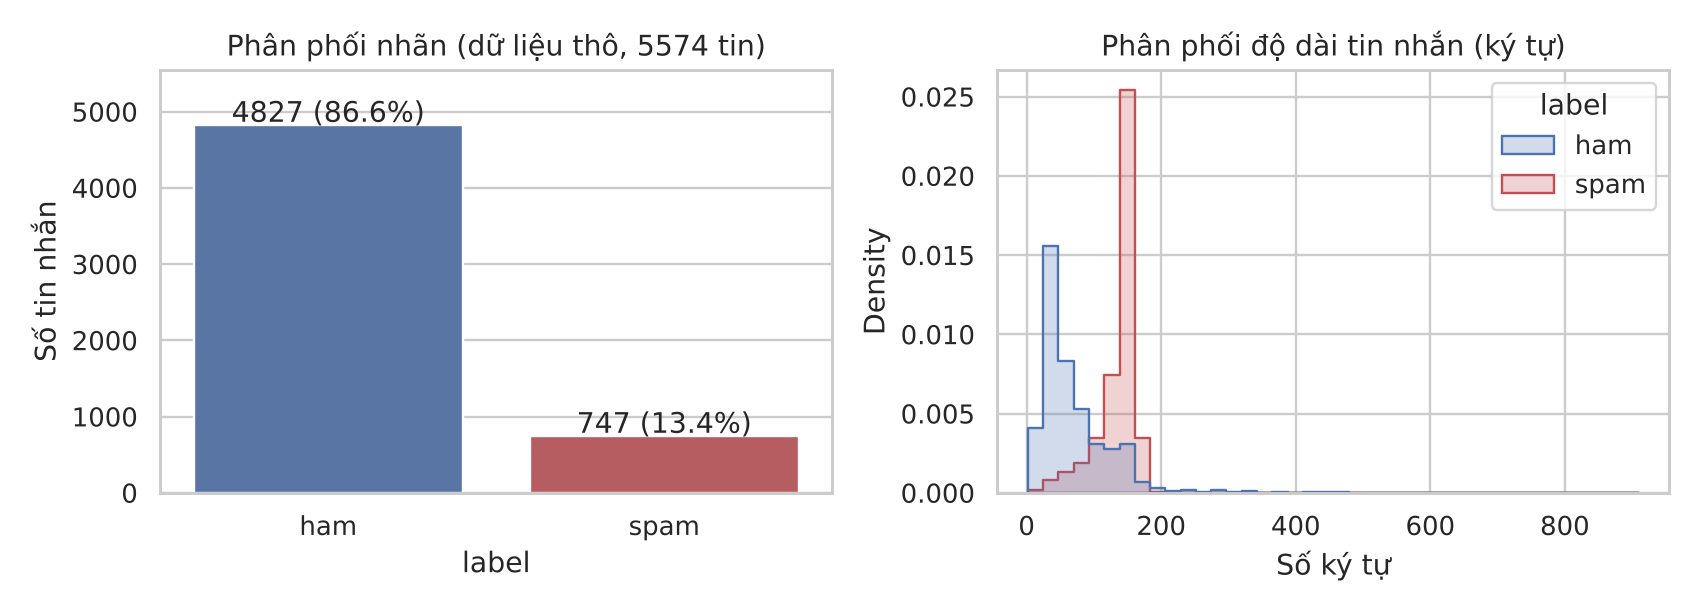
\includegraphics[width=0.95\textwidth]{images/eda_label_length.png}
    \caption{Phân phối nhãn dữ liệu thô (trái) và biểu đồ phân phối độ dài tin nhắn theo lớp (phải)}
    \label{fig:eda-label-length}
    \Nguon{Trích xuất tự động từ module thực nghiệm run\_experiments.py}
\end{figure}

Sự mất cân bằng này dẫn tới một hệ quả toán học và phương pháp luận cực kỳ quan trọng:
\begin{itemize}
    \item Giả sử xây dựng một bộ phân loại mù mờ (Naive Dummy Classifier) luôn luôn đưa ra kết quả dự đoán là \texttt{ham} cho mọi tin nhắn mà không cần đọc nội dung, bộ phân loại này vẫn đạt được độ chính xác (Accuracy) lên tới \textbf{87,4\%} trên tập huấn luyện và \textbf{87,3\%} trên tập kiểm thử!
    \item Tuy nhiên, một mô hình như vậy hoàn toàn vô dụng trong thực tiễn vì tỷ lệ bỏ sót tin nhắn rác là 100\% (Recall của spam bằng 0).
    \item Do đó, nhóm đi đến kết luận phương pháp luận cốt lõi: \textbf{Tuyệt đối không sử dụng độ chính xác (Accuracy) làm độ đo duy nhất hoặc tiêu chí chính để tối ưu hóa và so sánh mô hình}. Thay vào đó, nhóm thiết lập chỉ số F1-score của lớp dương (Spam) cùng với Precision, Recall, ma trận nhầm lẫn và diện tích dưới đường cong ROC (ROC-AUC) làm các thước đo trung tâm để đánh giá chất lượng mô hình.
\end{itemize}

\subsection{Phân tích đặc trưng hình thái và tín hiệu cấu trúc văn bản}
Để tìm kiếm các đặc trưng có khả năng phân biệt mạnh giữa hai lớp, nhóm đã tiến hành phân tích sâu về hình thái văn bản, độ dài tin nhắn và tần suất xuất hiện của các thành phần phi từ ngữ.
Các chỉ số thống kê mô tả được tổng hợp chi tiết trong Bảng~\ref{tab:tin-hieu-cau-truc}.

\begin{table}[H]
\centering
\caption{Đặc trưng hình thái và tỷ lệ xuất hiện các tín hiệu cấu trúc giữa hai lớp}
\label{tab:tin-hieu-cau-truc}
\begin{tabular}{|l|c|c|l|}
\hline
\textbf{Đặc trưng thống kê} & \textbf{Tin hợp lệ (Ham)} & \textbf{Tin rác (Spam)} & \textbf{Nhận xét phân hóa} \\
\hline
Độ dài trung bình (ký tự) & 70,9 & 137,7 & Spam dài gấp đôi Ham \\
\hline
Độ dài trung vị (ký tự) & 53,0 & 148,0 & Spam tập trung sát ngưỡng 160 \\
\hline
Độ dài lớn nhất (ký tự) & 910,0 & 223,0 & Ham có đuôi dài do viết tự do \\
\hline
Số lượng từ trung bình & 14,2 & 23,7 & Spam có mật độ từ ngữ cao hơn \\
\hline
Chứa chuỗi số dài ($\ge 5$ chữ số) & 0,1\% & 76,7\% & Tín hiệu phân biệt cực kỳ mạnh \\
\hline
Chứa địa chỉ web hoặc tên miền (URL) & 0,3\% & 17,8\% & Tỷ lệ xuất hiện ở Spam gấp 59 lần \\
\hline
Chứa ký hiệu tiền tệ (£, \$, €) & 0,4\% & 33,2\% & Tỷ lệ xuất hiện ở Spam gấp 83 lần \\
\hline
Tỷ lệ ký tự viết HOA trung bình & 7,7\% & 16,6\% & Spam lạm dụng chữ hoa để gây chú ý \\
\hline
\end{tabular}
\Nguon{Trích xuất tự động từ module run\_experiments.py}
\end{table}

Từ biểu đồ phân phối tại Hình~\ref{fig:eda-label-length} và các chỉ số trong Bảng~\ref{tab:tin-hieu-cau-truc}, nhóm rút ra các quan sát sâu sắc sau:
\begin{enumerate}
    \item \textbf{Về độ dài văn bản:} Các tin nhắn hợp lệ (\texttt{ham}) mang tính chất đối thoại thường nhật, thường rất ngắn gọn (trung vị chỉ 53 ký tự, 11 từ), nhưng phân phối có độ lệch phải rất lớn với một số tin nhắn dài tới 910 ký tự. Ngược lại, tin nhắn rác (\texttt{spam}) có phân phối độ dài rất tập trung quanh ngưỡng 130 đến 160 ký tự (trung bình 137,7 ký tự, trung vị 148 ký tự). Điều này phản ánh rõ nét thói quen của các đối tượng phát tán tin rác: cố gắng tận dụng tối đa giới hạn 160 ký tự của một bản tin SMS tiêu chuẩn để truyền tải càng nhiều thông tin quảng cáo, mời chào càng tốt.
    \item \textbf{Về tín hiệu chuỗi số dài (Long numeric sequences):} Có tới \textbf{76,7\%} tin nhắn rác chứa các chuỗi số từ 5 chữ số liên tiếp trở lên (đại diện cho số điện thoại hotline, đầu số tổng đài nhắn tin trả thưởng hoặc mã dịch vụ), trong khi ở tin nhắn thông thường tỷ lệ này chỉ là \textbf{0,1\%} (chênh lệch tới hơn 760 lần).
    \item \textbf{Về tín hiệu địa chỉ web (URL) và tiền tệ (Currency):} Tin nhắn rác xuất hiện dày đặc các ký hiệu tiền tệ (£, \$, €) chiếm 33,2\% (so với 0,4\% ở tin thường) và các đường dẫn website hoặc tên miền chiếm 17,8\% (so với 0,3\% ở tin thường).
    \item \textbf{Về phong cách biểu cảm:} Tin nhắn rác có tỷ lệ ký tự viết hoa trung bình lên tới 16,6\% (gấp hơn 2 lần tin thường), do các đối tượng gửi tin rác cố tình sử dụng các từ viết hoa toàn bộ như *“WINNER”*, *“FREE”*, *“URGENT”*, *“CLAIM NOW”* nhằm kích thích thị giác và thao túng tâm lý người nhận.
\end{enumerate}

\subsection{Khảo sát phân phối từ vựng đặc trưng theo lớp}
Bên cạnh các đặc trưng cấu trúc bề mặt, nhóm đã phân tích phân phối tần suất của các từ vựng xuất hiện nhiều nhất trong từng lớp (sau khi áp dụng chuẩn hóa và loại bỏ từ dừng tiếng Anh). Kết quả được trực quan hóa tại Hình~\ref{fig:eda-top-words}.

\begin{figure}[H]
    \centering
    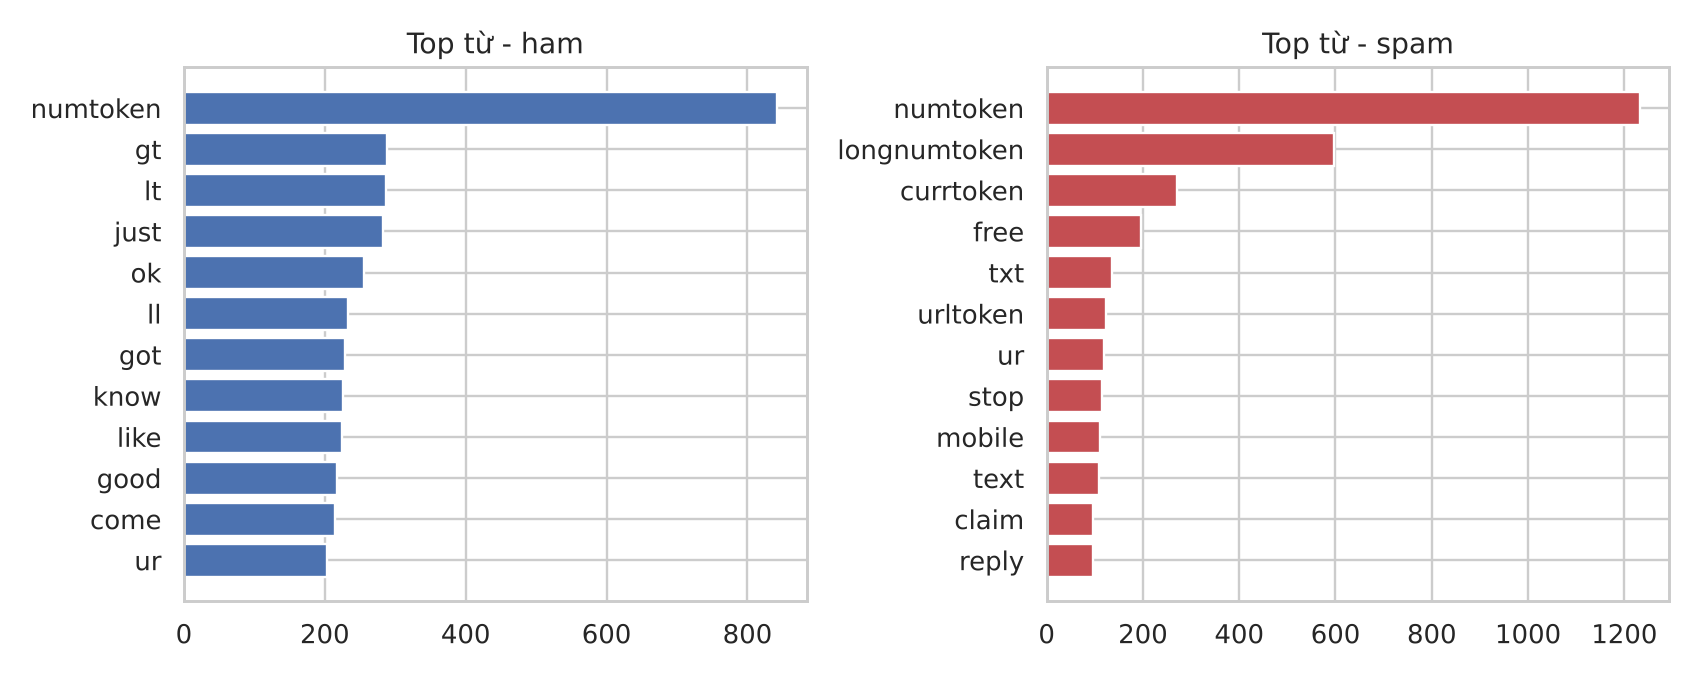
\includegraphics[width=0.9\textwidth]{images/eda_top_words.png}
    \caption{Top các từ vựng xuất hiện nhiều nhất trong lớp tin hợp lệ (trái) và lớp tin nhắn rác (phải)}
    \label{fig:eda-top-words}
    \Nguon{Trích xuất tự động từ module run\_experiments.py}
\end{figure}

Phân tích Hình~\ref{fig:eda-top-words} cho thấy sự phân cực từ vựng sâu sắc giữa hai thế giới văn bản:
\begin{itemize}
    \item \textbf{Thế giới của tin nhắn hợp lệ (Ham):} Bị chi phối bởi các từ ngữ giao tiếp thường nhật, chỉ địa điểm, thời gian, hoạt động cá nhân và cảm xúc thân mật: \texttt{home}, \texttt{come}, \texttt{later}, \texttt{ok}, \texttt{good}, \texttt{like}, \texttt{know}, \texttt{love}, \texttt{going}. Đặc biệt, xuất hiện hai token \texttt{gt} và \texttt{lt} với tần suất rất cao (nhóm sẽ phân tích nguyên nhân kỹ thuật của hiện tượng này ở Chương~\ref{chap:chuong5}).
    \item \textbf{Thế giới của tin nhắn rác (Spam):} Bị chi phối hoàn toàn bởi các thuật ngữ tiếp thị, tài chính, mệnh lệnh hành động và hứa hẹn lợi ích: \texttt{free}, \texttt{txt}, \texttt{claim}, \texttt{prize}, \texttt{won}, \texttt{mobile}, \texttt{urgent}, \texttt{cash}, \texttt{reply}, \texttt{contact}.
\end{itemize}

\section{Thiết lập hệ giả thuyết nghiên cứu}
\label{sec:gia-thuyet}

Dựa trên các bằng chứng định lượng thu nhận được từ quá trình khám phá dữ liệu (EDA), nhóm chính thức thiết lập hệ thống ba giả thuyết nghiên cứu (Research Hypotheses) làm kim chỉ nam xuyên suốt toàn bộ quá trình thiết kế giải pháp và thực nghiệm mô hình:

\begin{itemize}
    \item \textbf{Giả thuyết H1 (Bảo toàn tín hiệu cấu trúc qua kỹ thuật gom token đặc biệt):}
    \textit{“Do các chuỗi số điện thoại cụ thể, đường dẫn URL hoặc giá trị tiền tệ cụ thể hiếm khi lặp lại y hệt giữa các tin nhắn (tạo ra các từ vựng thưa thớt, vô nghĩa nếu để nguyên), việc áp dụng biểu thức chính quy (Regex) để quy đổi toàn bộ các thực thể này về các token tín hiệu chung có chủ đích (như \texttt{longnumtoken}, \texttt{urltoken}, \texttt{currtoken}, \texttt{numtoken}) sẽ giữ lại triệt để thông tin ngữ nghĩa then chốt, giúp cải thiện rõ rệt hiệu năng của các mô hình phân loại (đặc biệt là Cây quyết định và Naive Bayes) so với phương án xử lý thô hoặc xóa bỏ ký tự đặc biệt một cách máy móc.”}
    
    \item \textbf{Giả thuyết H2 (Hiệu quả của không gian n-gram kết hợp unigram và bigram):}
    \textit{“Các cụm từ cố định trong tin nhắn rác thường xuất hiện dưới dạng các cụm 2 từ có tính cảnh báo cao (ví dụ: *“cash prize”*, *“claim now”*, *“urgent call”*). Do đó, việc mở rộng không gian biểu diễn từ unigram đơn thuần sang kết hợp unigram + bigram sẽ giúp mô hình học được mối liên kết ngữ cảnh cục bộ, từ đó nâng cao độ chính xác nhận diện tin nhắn rác.”}
    
    \item \textbf{Giả thuyết H3 (Tầm quan trọng của cân đối chi phí lỗi và tiêu chí tối ưu hóa F1):}
    \textit{“Trong bài toán thực tế, chi phí của lỗi Dương tính giả (FP --- chặn nhầm một tin nhắn công việc hay giao dịch quan trọng) gây tổn thất lớn hơn rất nhiều so với lỗi Âm tính giả (FN --- để lọt một tin nhắn rác vào hòm thư). Do đó, việc tối ưu hóa siêu tham số bằng Cross-Validation cần căn cứ trên độ đo F1-score của lớp spam kết hợp giám sát chặt chẽ Precision, thay vì tối ưu hóa theo Accuracy thuần túy.”}
\end{itemize}

\section{Tóm tắt chương 1}
Chương 1 đã thiết lập toàn diện bức tranh tổng quan của đề tài nghiên cứu. Bộ dữ liệu SMS Spam Collection gồm 5.574 tin nhắn đã được làm sạch, loại bỏ 403 mẫu trùng lặp nhằm triệt tiêu nguy cơ rò rỉ dữ liệu, còn lại 5.171 mẫu duy nhất. Quá trình EDA đã chứng minh tính chất mất cân bằng nhãn sâu sắc (12,6\% spam) và nhận diện được các tín hiệu cấu trúc mang tính bản chất: tin nhắn rác dài hơn rõ rệt, chứa tới 76,7\% chuỗi số dài, 33,2\% ký hiệu tiền tệ và 17,8\% liên kết web. Hệ giả thuyết H1, H2, H3 được xác lập sẽ là nền tảng định hướng cho toàn bộ các bước thiết kế lý thuyết, xây dựng pipeline và thử nghiệm mô hình trong các chương tiếp theo.
\chapter{CƠ SỞ LÝ THUYẾT VÀ CÁC THUẬT TOÁN HỌC MÁY}
\label{chap:chuong2}

\section{Tổng quan về quy trình phân loại văn bản trong NLP}
\label{sec:quy-trinh-nlp}

Phân loại văn bản (Text Classification) là một trong những bài toán kinh điển và căn bản nhất của lĩnh vực Xử lý ngôn ngữ tự nhiên (Natural Language Processing --- NLP) và Học máy có giám sát (Supervised Machine Learning). Mục tiêu của bài toán là xây dựng một hàm ánh xạ $f: \mathcal{X} \rightarrow \mathcal{Y}$, trong đó miền đầu vào $\mathcal{X}$ là tập hợp các chuỗi ký tự hoặc văn bản ngôn ngữ tự nhiên có cấu trúc phi định hình, và miền đầu ra $\mathcal{Y}$ là một tập hữu hạn các nhãn lớp rời rạc $\mathcal{Y} = \{c_1, c_2, \dots, c_K\}$. Trong bài toán phân loại tin nhắn rác SMS, tập nhãn là nhị phân:
\begin{equation}
\mathcal{Y} = \{0: \text{ham (tin hợp lệ)}, \quad 1: \text{spam (tin nhắn rác)}\}
\end{equation}

Do các thuật toán học máy về bản chất chỉ có thể tính toán trên các vector số thực trong không gian vector nhiều chiều $\mathbb{R}^d$, một quy trình phân loại văn bản chuẩn mực luôn phải trải qua bốn chặng chuyển đổi kế tiếp nhau:
\begin{enumerate}
    \item \textbf{Tiền xử lý văn bản (Text Preprocessing):} Làm sạch nhiễu, chuẩn hóa hình thái từ vựng, chuyển đổi ký tự hoa/thường và thay thế các thành phần phi từ ngữ.
    \item \textbf{Biểu diễn đặc trưng (Feature Representation / Vectorization):} Ánh xạ các chuỗi từ vựng thành các vector số học đại diện (như Bag-of-Words hoặc TF-IDF) phản ánh phân phối và tầm quan trọng của các thuật ngữ.
    \item \textbf{Huấn luyện mô hình (Model Training):} Áp dụng các thuật toán học máy để tối ưu hóa hàm mục tiêu, học các ranh giới quyết định (Decision Boundaries) phân tách các lớp trong không gian đặc trưng.
    \item \textbf{Đánh giá và kiểm chứng (Evaluation):} Kiểm nghiệm hiệu năng tổng quát hóa trên dữ liệu độc lập thông qua hệ thống các độ đo thống kê phù hợp.
\end{enumerate}

\section{Các kỹ thuật tiền xử lý văn bản}
\label{sec:tien-xu-ly-ly-thuyet}

Tiền xử lý văn bản giữ vai trò quyết định đến chất lượng của không gian đặc trưng. Một câu văn thô chứa vô số thông tin dư thừa, các dị thường về kiểu gõ, dấu câu ngẫu nhiên hoặc các thực thể biến thiên liên tục. Nếu đưa trực tiếp văn bản thô vào bộ trích xuất đặc trưng, kích thước từ điển (Vocabulary) sẽ bùng nổ mất kiểm soát, sinh ra một không gian vector cực kỳ thưa thớt (Sparse space) chứa đầy nhiễu.

\subsection{Chuẩn hóa chữ thường và làm sạch cơ bản}
Bước sơ đẳng nhất trong xử lý văn bản là chuyển đổi toàn bộ ký tự về dạng chữ thường (Lowercasing). Trong tiếng Anh, việc viết hoa chữ cái đầu câu (như *“Call”* so với *“call”*) không mang lại sự khác biệt về mặt bản thể từ vựng. Chuẩn hóa chữ thường giúp quy tụ các biến thể này về một từ duy nhất, giảm kích thước từ vựng và khắc phục hiện tượng thưa dữ liệu. Kế đến, các ký tự ngắt dòng (\texttt{\textbackslash{}n}, \texttt{\textbackslash{}r}), khoảng trắng thừa liên tiếp được chuẩn hóa thành một dấu cách đơn giản (\texttt{\textbackslash{}s+} $\rightarrow$ \texttt{' '}).

\subsection{Kỹ thuật bảo toàn tín hiệu bằng Token thay thế có chủ đích}
Một sai lầm rất phổ biến trong xử lý văn bản truyền thống là việc loại bỏ máy móc toàn bộ các ký tự số và dấu câu thông qua các hàm xóa ký tự không phải chữ cái (\texttt{[\textasciicircum{}a-z]}). Trong bài toán phát hiện tin nhắn rác, điều này dẫn tới việc xóa sạch các thông tin sống còn:
\begin{itemize}
    \item Một số điện thoại cụ thể như \texttt{09061701461} hay \texttt{08712400603} hầu như chỉ xuất hiện 1 lần duy nhất trong toàn bộ tập dữ liệu. Nếu giữ nguyên, mỗi số điện thoại này sẽ trở thành một từ vựng riêng biệt có tần suất $1$ (cực kỳ hiếm), hoàn toàn vô dụng cho việc học quy luật tổng quát.
    \item Nhưng nếu xóa bỏ hoàn toàn số, mô hình sẽ mất trắng thông tin rằng *“tin nhắn này có chứa một số điện thoại dài mời gọi liên hệ”*.
\end{itemize}

Để giải quyết mâu thuẫn này, nhóm đã nghiên cứu và ứng dụng kỹ thuật \textbf{Bảo toàn tín hiệu cấu trúc (Signal-preserving Tokenization)} thông qua biểu thức chính quy (Regex). Cụ thể:
\begin{enumerate}
    \item \textbf{Token hóa liên kết Web/Domain (\texttt{urltoken}):}
    Sử dụng biểu thức chính quy phát hiện toàn bộ các định dạng URL bắt đầu bằng \texttt{http://}, \texttt{https://}, \texttt{www.} hoặc các đuôi tên miền phổ biến (\texttt{.com}, \texttt{.co.uk}, \texttt{.net}, \texttt{.org}):
    \begin{equation}
    \text{URL\_RE} = \verb|r"(https?://\S+|www\.\S+|\b\S+\.(com|co\.uk|net|org)\b\S*)"|
    \end{equation}
    Mọi địa chỉ web được thay thế thống nhất bằng từ khóa đặc biệt \texttt{urltoken}.
    \item \textbf{Token hóa ký hiệu tiền tệ (\texttt{currtoken}):}
    Phát hiện các ký hiệu tiền tệ phổ biến trong tin nhắn lừa đảo và trao thưởng (£, \$, €):
    \begin{equation}
    \text{CURR\_RE} = \verb|r"[£$€]"|
    \end{equation}
    Được thay thế bằng token \texttt{currtoken}.
    \item \textbf{Token hóa chuỗi số dài liên tiếp (\texttt{longnumtoken}):}
    Phát hiện các chuỗi số có từ 5 chữ số liên tiếp trở lên (đại diện cho số điện thoại di động, đầu số tổng đài hoặc mã thẻ cào):
    \begin{equation}
    \text{LONGNUM\_RE} = \verb|r"\b\d{5,}\b"|
    \end{equation}
    Được thay thế bằng token \texttt{longnumtoken}.
    \item \textbf{Token hóa số thông thường (\texttt{numtoken}):}
    Các số ngắn còn lại (như giờ giấc, số lượng) được quy đổi về \texttt{numtoken}:
    \begin{equation}
    \text{NUM\_RE} = \verb|r"\b\d+\b"|
    \end{equation}
\end{enumerate}

Sau khi đã bảo toàn các tín hiệu cấu trúc dưới dạng các token đặc biệt, toàn bộ các dấu câu và ký tự phi chữ cái còn lại mới được loại bỏ an toàn. Kỹ thuật này chuyển hóa một tập hợp vô số các chuỗi số/URL ngẫu nhiên thành một số ít các đặc trưng thống kê có trọng số cực cao.

\subsection{Kỹ thuật loại bỏ từ dừng (Stop Words Removal)}
Từ dừng (Stop words) là các từ ngữ xuất hiện với tần suất rất cao trong ngôn ngữ tự nhiên nhưng mang rất ít giá trị phân biệt ngữ nghĩa (như các đại từ, giới từ, liên từ trong tiếng Anh: *“is”*, *“the”*, *“at”*, *“which”*, *“on”*). Việc loại bỏ danh sách từ dừng chuẩn tiếng Anh (English stop words) giúp:
\begin{itemize}
    \item Thu hẹp đáng kể số chiều của không gian đặc trưng;
    \item Tập trung trọng số học tập của mô hình vào các thực từ (Content words) mang tải trọng ngữ nghĩa lớn như động từ, danh từ và tính từ.
\end{itemize}
Tuy nhiên, trong xử lý văn bản, việc loại bỏ stop words đôi khi làm mất đi các đại từ mang tính tương tác cá nhân (ví dụ: sự khác biệt giữa *“you”*, *“me”*, *“call me”* so với *“free to you”*). Do đó, việc loại bỏ từ dừng cần được đưa vào thực nghiệm để đối sánh khách quan thay vì mặc định áp dụng.

\section{Các phương pháp biểu diễn đặc trưng văn bản}
\label{sec:bieu-dien-dac-trung}

\subsection{Mô hình túi từ (Bag-of-Words --- BoW)}
Mô hình túi từ (Bag-of-Words) là phương pháp biểu diễn văn bản cổ điển và nền tảng nhất. Cho một tập ngữ liệu gồm $M$ văn bản $\mathcal{D} = \{d_1, d_2, \dots, d_M\}$. Giả sử sau quá trình tiền xử lý, tập từ vựng duy nhất được xây dựng gồm $V$ từ: $\mathcal{V} = \{w_1, w_2, \dots, w_V\}$.

Trong mô hình BoW (được triển khai thông qua lớp \texttt{CountVectorizer} của scikit-learn), mỗi văn bản $d$ được biểu diễn thành một vector $V$ chiều:
\begin{equation}
\mathbf{x} = [x_1, x_2, \dots, x_V]^T \in \mathbb{N}^V
\end{equation}
trong đó mỗi phần tử $x_j$ thể hiện số lần xuất hiện (Term Frequency) của từ $w_j$ trong văn bản $d$:
\begin{equation}
x_j = \text{count}(w_j, d)
\end{equation}
Mô hình túi từ hoàn toàn bỏ qua thứ tự xuất hiện của các từ trong câu cũng như cấu trúc ngữ pháp, chỉ lưu giữ thông tin về sự hiện diện và số lượng đếm của các từ.

\subsection{Phương pháp trọng số TF-IDF}
Một nhược điểm cố hữu của mô hình túi từ BoW là việc gán trọng số thuần túy theo số lần xuất hiện: những từ xuất hiện quá nhiều trong mọi văn bản sẽ có giá trị rất lớn, lấn át các từ mang tính đặc thù cao. Để khắc phục điều này, phương pháp \textbf{TF-IDF (Term Frequency --- Inverse Document Frequency)} được sử dụng nhằm cân bằng giữa tần suất cục bộ của từ trong một văn bản và độ hiếm tổng thể của từ đó trong toàn bộ tập ngữ liệu.

Trọng số TF-IDF của từ $t$ trong văn bản $d$ thuộc tập ngữ liệu $\mathcal{D}$ được xác định bởi:
\begin{equation}
\text{TF-IDF}(t, d, \mathcal{D}) = \text{TF}(t, d) \times \text{IDF}(t, \mathcal{D})
\end{equation}

Trong thư viện \texttt{scikit-learn} (\texttt{TfidfVectorizer}), thành phần tần suất nghịch đảo tài liệu IDF được tính toán có làm trơn (Smooth IDF) theo công thức:
\begin{equation}
\text{IDF}(t, \mathcal{D}) = \ln \left( \frac{1 + |\mathcal{D}|}{1 + \text{DF}(t)} \right) + 1
\end{equation}
trong đó $|\mathcal{D}|$ là tổng số văn bản trong tập ngữ liệu huấn luyện, và $\text{DF}(t)$ (Document Frequency) là số lượng văn bản có chứa từ $t$. Giá trị $+1$ trong tử số và mẫu số giúp triệt tiêu hiện tượng chia cho 0, và số hạng $+1$ ở ngoài đảm bảo giá trị IDF luôn dương.

Sau khi tính toán trọng số TF-IDF thô cho từng từ trong văn bản, vector đặc trưng $\mathbf{x} = [v_1, v_2, \dots, v_V]$ được chuẩn hóa theo chuẩn Euclid ($L_2$-norm) để đưa độ dài vector về $1$:
\begin{equation}
\mathbf{x}_{\text{norm}} = \frac{\mathbf{x}}{\|\mathbf{x}\|_2} = \frac{[v_1, v_2, \dots, v_V]}{\sqrt{\sum_{j=1}^V v_j^2}}
\end{equation}
Chuẩn hóa $L_2$ đóng vai trò cốt tử: nó triệt tiêu ảnh hưởng của độ dài văn bản, giúp hai văn bản có cùng nội dung từ ngữ nhưng độ dài ngắn khác nhau sẽ có vector biểu diễn gần nhau trong không gian vector.

\subsection{Không gian n-gram và các tham số lọc từ vựng}
\begin{itemize}
    \item \textbf{Khái niệm n-gram:} Một n-gram là một chuỗi gồm $n$ từ liên tiếp xuất hiện cùng nhau trong văn bản.
    \begin{itemize}
        \item $n=1$ (Unigram): Từng từ đơn lẻ độc lập (ví dụ: *“claim”*, *“prize”*).
        \item $n=2$ (Bigram): Cặp 2 từ liền kề (ví dụ: *“claim prize”*, *“urgent call”*).
    \end{itemize}
    Việc kết hợp unigram và bigram (\texttt{ngram\_range=(1, 2)}) cho phép mô hình lưu giữ một phần ngữ cảnh cục bộ và các cụm từ cố định.
    \item \textbf{Tham số \texttt{min\_df} (Minimum Document Frequency):} Ngưỡng tần số tài liệu tối thiểu để một từ được đưa vào từ điển. Ví dụ \texttt{min\_df=2} quy định một từ phải xuất hiện ở ít nhất 2 văn bản khác nhau mới được giữ lại, giúp loại bỏ các từ gõ sai chính tả hoặc dị thường chỉ xuất hiện 1 lần.
    \item \textbf{Tham số \texttt{max\_df} (Maximum Document Frequency):} Ngưỡng tỷ lệ tài liệu tối đa. Ví dụ \texttt{max\_df=0.5} quy định loại bỏ các từ xuất hiện trong hơn 50\% tổng số văn bản của tập ngữ liệu (đóng vai trò như bộ lọc stop words tự động).
    \item \textbf{Tham số \texttt{max\_features}:} Giới hạn số lượng đặc trưng tối đa được chọn vào từ vựng, sắp xếp theo thứ tự giảm dần của tần suất xuất hiện.
\end{itemize}

\section{Thuật toán Multinomial Naive Bayes}
\label{sec:multinomial-nb}

\subsection{Định lý Bayes và giả định độc lập có điều kiện}
Thuật toán Naive Bayes là một mô hình phân loại xác suất dựa trên việc áp dụng Định lý Bayes (Bayes' Theorem). Cho một văn bản được biểu diễn dưới dạng vector đặc trưng $\mathbf{x} = (x_1, x_2, \dots, x_d)$. Theo định lý Bayes, xác suất hậu nghiệm (Posterior Probability) để mẫu $\mathbf{x}$ thuộc về lớp $y \in \{0, 1\}$ được tính theo công thức:
\begin{equation}
P(y | \mathbf{x}) = \frac{P(y) P(\mathbf{x} | y)}{P(\mathbf{x})} = \frac{P(y) P(x_1, x_2, \dots, x_d | y)}{\sum_{y'} P(y') P(\mathbf{x} | y')}
\end{equation}
trong đó:
\begin{itemize}
    \item $P(y)$ là xác suất tiền định (Prior Probability) của lớp $y$.
    \item $P(\mathbf{x} | y)$ là hàm khả năng (Likelihood) sinh ra vector $\mathbf{x}$ khi biết trước lớp $y$.
    \item $P(\mathbf{x})$ là hằng số chuẩn hóa độc lập với lớp $y$.
\end{itemize}

Để giải quyết bài toán tính toán phân phối đồng thời phức tạp $P(x_1, x_2, \dots, x_d | y)$, thuật toán đưa ra \textbf{Giả định ngây thơ (Naive Conditional Independence Assumption)}: Mọi đặc trưng $x_i$ đều độc lập có điều kiện với nhau khi biết trước nhãn lớp $y$:
\begin{equation}
P(\mathbf{x} | y) = \prod_{i=1}^d P(x_i | y)
\end{equation}

Từ giả định này, quy tắc ra quyết định Bayes (Maximum A Posteriori --- MAP) để tìm lớp dự đoán $\hat{y}$ trở thành:
\begin{equation}
\hat{y} = \arg\max_{y \in \{0, 1\}} P(y | \mathbf{x}) = \arg\max_{y \in \{0, 1\}} \left[ P(y) \prod_{i=1}^d P(x_i | y) \right]
\end{equation}
Chuyển sang miền Log-space để tránh hiện tượng tràn số dưới (Arithmetic Underflow) khi nhân liên tiếp nhiều xác suất nhỏ:
\begin{equation}
\hat{y} = \arg\max_{y \in \{0, 1\}} \left[ \ln P(y) + \sum_{i=1}^d \ln P(x_i | y) \right]
\end{equation}

\subsection{Biến thể Multinomial Naive Bayes và kỹ thuật làm trơn Laplace}
Đối với dữ liệu văn bản được biểu diễn dưới dạng tần số đếm hoặc vector TF-IDF, biến thể \textbf{Multinomial Naive Bayes (MNB)} mô hình hóa quá trình sinh văn bản theo phân phối đa thức.
Xác suất khả năng sinh ra từ vựng $w_i$ khi biết trước nhãn $y$ được ước lượng bằng tỷ lệ số lần từ $w_i$ xuất hiện trong các văn bản thuộc lớp $y$ so với tổng số lượng từ của toàn bộ lớp $y$:
\begin{equation}
P(w_i | y) = \frac{N_{yi}}{N_y}
\end{equation}
trong đó $N_{yi}$ là tổng số lần từ $w_i$ xuất hiện trong lớp $y$, và $N_y = \sum_{j=1}^{|\mathcal{V}|} N_{yj}$ là tổng số từ xuất hiện trong lớp $y$.

\textbf{Vấn đề xác suất bằng 0 (Zero-Frequency Problem):} Nếu một từ $w_i$ chưa từng xuất hiện trong tập huấn luyện của lớp $y$, thì $N_{yi} = 0$, dẫn tới $P(w_i | y) = 0$. Khi tính tích xác suất cho toàn bộ câu, sự xuất hiện của từ mới này sẽ lập tức kéo toàn bộ tích xác suất về $0$, xóa sạch hoàn toàn mọi bằng chứng của các từ khóa khác trong câu!

Để khắc phục hiện tượng nguy hiểm này, kỹ thuật \textbf{Làm trơn Laplace (Laplace/Lidstone Smoothing)} được áp dụng thông qua việc cộng thêm một hằng số làm trơn $\alpha > 0$ vào tử số và $\alpha \times |\mathcal{V}|$ vào mẫu số:
\begin{equation}
\label{eq:laplace-smoothing}
\hat{P}(w_i | y) = \frac{N_{yi} + \alpha}{N_y + \alpha |\mathcal{V}|}
\end{equation}
trong đó:
\begin{itemize}
    \item Khi $\alpha = 1$, phép làm trơn được gọi là Làm trơn Laplace chuẩn (Add-1 smoothing);
    \item Khi $0 < \alpha < 1$ hoặc $\alpha > 1$, phép làm trơn được gọi là Làm trơn Lidstone.
    \item $|\mathcal{V}|$ là tổng kích thước của không gian từ vựng.
\end{itemize}

\subsection{Cơ chế phân tích trọng số từ qua Log-Odds Ratio}
Một ưu điểm vượt trội của mô hình Multinomial Naive Bayes là khả năng diễn giải rất sáng tỏ. Để định lượng mức độ một từ $w_i$ có xu hướng đẩy dự đoán về phía tin nhắn rác (\texttt{spam}) hay tin nhắn hợp lệ (\texttt{ham}), ta có thể tính tỷ số logarit cơ số tự nhiên giữa hai khả năng (Log-Odds Ratio):
\begin{equation}
\label{eq:log-odds}
\text{Log-Odds}(w_i) = \ln \hat{P}(w_i | y=1) - \ln \hat{P}(w_i | y=0)
\end{equation}
Nếu $\text{Log-Odds}(w_i) > 0$, sự xuất hiện của từ $w_i$ sẽ làm tăng xác suất dự đoán là spam. Giá trị này càng lớn, từ $w_i$ càng là tín hiệu đặc trưng cực mạnh của tin nhắn rác. Ngược lại, nếu $\text{Log-Odds}(w_i) < 0$, từ vựng sẽ kéo dự đoán về phía tin nhắn hợp lệ.

\section{Thuật toán K-Láng giềng gần nhất (K-Nearest Neighbors)}
\label{sec:knn-ly-thuyet}

\subsection{Nguyên lý phân loại dựa trên không gian hình học}
Thuật toán K-NN là một thuật toán học lười (Lazy Learning / Instance-based Learning). Mô hình không trải qua quá trình tối ưu hóa trọng số tường minh trong giai đoạn huấn luyện, mà lưu trữ toàn bộ tập dữ liệu huấn luyện $\mathcal{D}_{\text{train}} = \{(\mathbf{x}_i, y_i)\}_{i=1}^N$ vào bộ nhớ. Khi có một mẫu mới $\mathbf{x}_{\text{test}}$ cần dự đoán, thuật toán tiến hành đo khoảng cách từ $\mathbf{x}_{\text{test}}$ tới mọi điểm dữ liệu trong tập huấn luyện, lựa chọn ra $K$ điểm có khoảng cách gần nhất, và ra quyết định dựa trên cơ chế biểu quyết (Voting).

\subsection{Các độ đo khoảng cách và vấn đề “Khoảng cách công bằng”}
Hiệu năng của thuật toán K-NN phụ thuộc hoàn toàn vào hàm khoảng cách (Distance Metric) được lựa chọn trên không gian đặc trưng.
\begin{enumerate}
    \item \textbf{Khoảng cách Euclid (Euclidean Distance):}
    Khoảng cách hình học thông thường giữa hai vector $\mathbf{u}, \mathbf{v} \in \mathbb{R}^d$:
    \begin{equation}
    d_{\text{Euclid}}(\mathbf{u}, \mathbf{v}) = \|\mathbf{u} - \mathbf{v}\|_2 = \sqrt{\sum_{j=1}^d (u_j - v_j)^2}
    \end{equation}
    \item \textbf{Khoảng cách Cosine (Cosine Distance):}
    Dựa trên góc giữa hai vector trong không gian đa chiều, bất biến đối với độ lớn (Magnitude) của vector:
    \begin{equation}
    \text{Sim}_{\text{Cosine}}(\mathbf{u}, \mathbf{v}) = \frac{\mathbf{u} \cdot \mathbf{v}}{\|\mathbf{u}\|_2 \|\mathbf{v}\|_2} = \frac{\sum_{j=1}^d u_j v_j}{\sqrt{\sum_{j=1}^d u_j^2} \sqrt{\sum_{j=1}^d v_j^2}}
    \end{equation}
    \begin{equation}
    d_{\text{Cosine}}(\mathbf{u}, \mathbf{v}) = 1 - \text{Sim}_{\text{Cosine}}(\mathbf{u}, \mathbf{v})
    \end{equation}
\end{enumerate}

\textbf{Nghịch lý khoảng cách Euclid trên dữ liệu văn bản thưa:}
Trong Bài giảng số 3 của học phần, giảng viên đã nhấn mạnh vấn đề: *“Khoảng cách có công bằng không?”*. Trong bài toán phân loại văn bản biểu diễn bằng BoW (vector đếm):
\begin{itemize}
    \item Xét hai tin nhắn hợp lệ: một tin nhắn rất ngắn (ví dụ: *“Call me”* --- 2 từ) và một tin nhắn dài (ví dụ: *“Call me when you get home, I will be at the library studying”* --- 13 từ). Mặc dù cùng là tin nhắn gia đình hợp lệ, nhưng do độ dài khác nhau, vector đếm của chúng có độ lớn cách xa nhau, khiến khoảng cách Euclid $d_{\text{Euclid}}$ giữa chúng rất lớn.
    \item Ngược lại, một tin nhắn spam ngắn (ví dụ: *“Call 09061”*) lại có độ lớn vector gần với tin nhắn ngắn hợp lệ hơn!
    \item Do đó, khoảng cách Euclid bị chi phối bởi độ dài văn bản thay vì nội dung ngữ nghĩa. Để K-NN hoạt động hiệu quả trên văn bản, bắt buộc phải kết hợp vector hóa TF-IDF chuẩn hóa $L_2$ với \textbf{Độ đo Cosine (Cosine metric)}.
\end{itemize}

\subsection{Cơ chế biểu quyết và trọng số láng giềng}
Xác suất dự đoán mẫu thuộc lớp spam $P(y=1 | \mathbf{x})$ trong K-NN được xác định qua $K$ láng giềng gần nhất $\mathcal{N}_K(\mathbf{x})$:
\begin{itemize}
    \item \textbf{Biểu quyết đồng đều (\texttt{weights='uniform'}):}
    \begin{equation}
    P(y=1 | \mathbf{x}) = \frac{1}{K} \sum_{i \in \mathcal{N}_K(\mathbf{x})} \mathbb{I}(y_i = 1)
    \end{equation}
    \item \textbf{Biểu quyết theo trọng số nghịch đảo khoảng cách (\texttt{weights='distance'}):}
    Các điểm nằm càng gần mẫu thử nghiệm sẽ có tiếng nói càng có trọng lượng trong kết quả biểu quyết:
    \begin{equation}
    w_i = \frac{1}{d(\mathbf{x}, \mathbf{x}_i) + \epsilon}
    \end{equation}
    \begin{equation}
    P(y=1 | \mathbf{x}) = \frac{\sum_{i \in \mathcal{N}_K(\mathbf{x})} w_i \mathbb{I}(y_i = 1)}{\sum_{i \in \mathcal{N}_K(\mathbf{x})} w_i}
    \end{equation}
\end{itemize}

\section{Thuật toán Cây quyết định (Decision Tree)}
\label{sec:decision-tree-ly-thuyet}

\subsection{Cấu trúc cây và cơ chế phân tách nút}
Cây quyết định (Decision Tree) là mô hình học máy phi tham số xây dựng cấu trúc phân cấp dạng cây để phân chia không gian dữ liệu thành các siêu hình hộp chữ nhật đồng nhất.
Cấu trúc cây gồm:
\begin{itemize}
    \item \textbf{Nút gốc (Root Node):} Chứa toàn bộ tập dữ liệu huấn luyện ban đầu.
    \item \textbf{Các nút quyết định (Decision Nodes):} Áp dụng một điều kiện kiểm tra nhị phân trên một đặc trưng cụ thể (ví dụ: $\text{count}(\text{longnumtoken}) \le 0.5$).
    \item \textbf{Các nút lá (Leaf Nodes):} Các nút kết thúc không phân chia thêm, gán nhãn dự đoán cho mẫu dữ liệu dựa trên tỷ lệ chiếm ưu thế của các mẫu rơi vào nút đó.
\end{itemize}

Tại mỗi nút phân chia, thuật toán duyệt qua toàn bộ các đặc trưng và các ngưỡng phân chia có thể để tìm ra phép phân tách dữ liệu tối ưu sao cho độ tinh khiết (Purity) của các tập con thu được là lớn nhất.

\subsection{Các tiêu chí đánh giá độ tinh khiết (Impurity Criteria)}
\begin{enumerate}
    \item \textbf{Độ mờ Gini (Gini Impurity):}
    Đo lường xác suất một mẫu được chọn ngẫu nhiên bị gán nhãn sai nếu được gán nhãn ngẫu nhiên theo phân phối của nút:
    \begin{equation}
    \text{Gini}(D) = 1 - \sum_{k=0}^1 p_k^2 = 1 - (p_0^2 + p_1^2)
    \end{equation}
    trong đó $p_k$ là tỷ lệ mẫu thuộc lớp $k$ tại nút $D$. Giá trị $\text{Gini} = 0$ khi nút hoàn toàn thuần khiết (chỉ chứa một lớp duy nhất).
    \item \textbf{Entropy và Độ lợi thông tin (Information Gain):}
    Dựa trên lý thuyết thông tin Shannon, độ hỗn loạn thông tin Entropy được tính bởi:
    \begin{equation}
    H(D) = -\sum_{k=0}^1 p_k \log_2(p_k)
    \end{equation}
    Độ lợi thông tin (Information Gain) khi phân chia tập $D$ thành hai tập con $D_{\text{left}}$ và $D_{\text{right}}$ theo thuộc tính $A$ là:
    \begin{equation}
    IG(D, A) = H(D) - \left( \frac{|D_{\text{left}}|}{|D|} H(D_{\text{left}}) + \frac{|D_{\text{right}}|}{|D|} H(D_{\text{right}}) \right)
    \end{equation}
\end{enumerate}

\subsection{Kiểm soát quá khớp (Overfitting) và Độ quan trọng đặc trưng}
Trong không gian văn bản có hàng nghìn chiều, Cây quyết định rất dễ bị quá khớp (Overfitting): cây phát triển quá sâu để ghi nhớ từng trường hợp cá biệt của tập huấn luyện, dẫn tới hiệu năng trên tập kiểm thử bị sụt giảm nghiêm trọng.
Để khắc phục, các siêu tham số chặn sớm (Pre-pruning) được thiết lập:
\begin{itemize}
    \item \texttt{max\_depth}: Giới hạn độ sâu tối đa của cây (ví dụ \texttt{max\_depth=10}).
    \item \texttt{min\_samples\_leaf}: Số lượng mẫu tối thiểu bắt buộc phải có tại một nút lá (tránh tạo ra các nút lá chỉ đại diện cho 1 mẫu cá biệt).
\end{itemize}

Bên cạnh đó, Cây quyết định cung cấp chỉ số \textbf{Độ quan trọng đặc trưng (Feature Importance)}, được tính bằng tổng mức suy giảm độ mờ Gini (Mean Decrease Impurity) mà đặc trưng đó đóng góp trên toàn bộ các nút phân chia của cây:
\begin{equation}
\text{Importance}(f) = \sum_{t \in T, v(t)=f} \frac{N_t}{N} \left( \text{Gini}(t) - \frac{N_{t_L}}{N_t} \text{Gini}(t_L) - \frac{N_{t_R}}{N_t} \text{Gini}(t_R) \right)
\end{equation}

\section{Hệ thống độ đo đánh giá mô hình phân loại nhị phân}
\label{sec:do-do-ly-thuyet}

Để đánh giá toàn diện năng lực của các mô hình học máy trên tập dữ liệu mất cân bằng, việc xây dựng một hệ thống độ đo chuẩn xác là điều kiện tiên quyết.

\subsection{Ma trận nhầm lẫn (Confusion Matrix)}
Ma trận nhầm lẫn tổng hợp kết quả đối sánh giữa nhãn thực tế và nhãn dự đoán trên tập kiểm thử thành bảng 4 ô:
\begin{table}[H]
\centering
\caption{Cấu trúc ma trận nhầm lẫn cho bài toán phân loại nhị phân SMS Spam}
\label{tab:ly-thuyet-cm}
\begin{tabular}{|c|c|c|}
\hline
\multirow{2}{*}{\textbf{Thực tế (Ground Truth)}} & \multicolumn{2}{c|}{\textbf{Dự đoán (Predicted)}} \\
\cline{2-3}
& \textbf{Dự đoán là Ham ($y=0$)} & \textbf{Dự đoán là Spam ($y=1$)} \\
\hline
\textbf{Thực tế là Ham ($y=0$)} & \textbf{TN} (True Negative) & \textbf{FP} (False Positive --- Báo nhầm) \\
\hline
\textbf{Thực tế là Spam ($y=1$)} & \textbf{FN} (False Negative --- Bỏ sót) & \textbf{TP} (True Positive) \\
\hline
\end{tabular}
\end{table}

Trong bối cảnh thực tiễn của dịch vụ lọc tin nhắn:
\begin{itemize}
    \item \textbf{Lỗi Dương tính giả (False Positive --- FP / Type I Error):} Hệ thống dự đoán một tin nhắn bình thường là spam và chặn lại. Đây là lỗi cực kỳ nguy hiểm, có thể làm người dùng bỏ lỡ mã OTP ngân hàng, tin nhắn công việc khẩn cấp hoặc tin tức gia đình.
    \item \textbf{Lỗi Âm tính giả (False Negative --- FN / Type II Error):} Hệ thống bỏ sót một tin nhắn rác vào hòm thư. Lỗi này gây phiền toái cho người dùng nhưng ít gây ra hậu quả thảm họa như lỗi FP.
\end{itemize}

\subsection{Độ chính xác (Accuracy)}
\begin{equation}
\text{Accuracy} = \frac{\text{TP} + \text{TN}}{\text{TP} + \text{TN} + \text{FP} + \text{FN}}
\end{equation}
Tỷ lệ dự đoán đúng trên toàn bộ tập dữ liệu. Như đã chứng minh ở Chương 1, độ đo này không phản ánh trung thực hiệu năng khi dữ liệu mất cân bằng.

\subsection{Độ chuẩn xác (Precision)}
\begin{equation}
\text{Precision} = \frac{\text{TP}}{\text{TP} + \text{FP}}
\end{equation}
Tỷ lệ tin nhắn thực sự là spam trong số tất cả các tin nhắn mà mô hình đã gắn nhãn spam. Precision phản ánh mức độ đáng tin cậy khi mô hình phát chuông báo động spam (tránh báo động giả).

\subsection{Độ bao phủ (Recall / Sensitivity)}
\begin{equation}
\text{Recall} = \frac{\text{TP}}{\text{TP} + \text{FN}}
\end{equation}
Tỷ lệ tin nhắn rác mà mô hình bắt giữ thành công trên tổng số tin nhắn rác thực tế có trong tập dữ liệu. Recall phản ánh khả năng quét sạch tin rác của bộ lọc (tránh bỏ lọt tội phạm).

\subsection{Điểm số F1 (F1-Score)}
Precision và Recall thường có mối quan hệ đánh đổi (Trade-off). Điểm F1 là trung bình điều hòa (Harmonic Mean) giữa Precision và Recall, đem lại một thước đo duy nhất cân bằng hoàn hảo giữa hai mục tiêu:
\begin{equation}
F_1 = 2 \times \frac{\text{Precision} \times \text{Recall}}{\text{Precision} + \text{Recall}} = \frac{2\text{TP}}{2\text{TP} + \text{FP} + \text{FN}}
\end{equation}
F1-score chỉ đạt giá trị cao khi cả Precision và Recall đều đồng thời đạt mức tốt.

\subsection{Đường cong ROC và chỉ số AUC}
Đường cong đặc trưng hoạt động của bộ thu (Receiver Operating Characteristic --- ROC) biểu diễn mối quan hệ phụ thuộc giữa Tỷ lệ Dương tính thật (True Positive Rate --- $\text{TPR} = \text{Recall}$) và Tỷ lệ Dương tính giả (False Positive Rate --- $\text{FPR} = \frac{\text{FP}}{\text{TN} + \text{FP}}$) khi thay đổi liên tục ngưỡng phân loại xác suất $\tau \in [0, 1]$.

Diện tích dưới đường cong ROC (Area Under the Curve --- ROC-AUC) nhận giá trị trong đoạn $[0.5, 1.0]$. Một mô hình đoán ngẫu nhiên có $\text{AUC} = 0.5$, và một mô hình hoàn hảo có $\text{AUC} = 1.0$. Chỉ số AUC phản ánh năng lực xếp hạng xác suất (Ranking capability) tổng thể của mô hình mà không phụ thuộc vào một ngưỡng cắt quyết định đơn lẻ.

\section{Tóm tắt chương 2}
Chương 2 đã thiết lập hệ thống cơ sở lý thuyết toán học và khoa học dữ liệu hoàn chỉnh cho bài toán phân loại văn bản. Nhóm đã làm sáng tỏ cơ chế hoạt động của mô hình biểu diễn túi từ BoW và trọng số TF-IDF; phân tích nền tảng xác suất của Multinomial Naive Bayes cùng kỹ thuật làm trơn Laplace và tỷ số Log-Odds; phân tích bản chất hình học của K-NN và nguyên nhân bắt buộc phải sử dụng khoảng cách Cosine trên vector TF-IDF; phân tích giải thuật chia nhánh của Cây quyết định với tiêu chí Gini/Entropy; và xây dựng hệ thống độ đo toàn diện với trọng tâm là F1-score và ma trận nhầm lẫn. Toàn bộ nền tảng lý thuyết này sẽ được cụ thể hóa thành kiến trúc hệ thống và quy trình thực nghiệm trong Chương 3.
\chapter{THIẾT KẾ GIẢI PHÁP VÀ QUY TRÌNH HỌC MÁY (PIPELINE)}
\label{chap:chuong3}

\section{Kiến trúc tổng thể của hệ thống}
\label{sec:kien-truc-he-thong}

Để giải quyết triệt để bài toán phân loại tin nhắn rác với độ tin cậy và tính tái lập cao nhất, Nhóm 13 đã thiết kế một kiến trúc học máy khép kín, phân tầng và tự động hóa cao. Toàn bộ quy trình từ dữ liệu thô ban đầu đến mô hình triển khai thực tế được trực quan hóa thông qua sơ đồ khối tại Sơ đồ~\ref{sd:quy-trinh-pipeline}.

\begin{sodo}[H]
\centering
\begin{tikzpicture}[
    node distance=0.6cm and 0.6cm,
    every node/.style={font=\footnotesize},
    box/.style={draw=blue!70!black, line width=0.8pt, rounded corners=3pt, align=center, minimum height=1.0cm, minimum width=2.0cm, fill=blue!5},
    process/.style={draw=orange!80!black, line width=0.8pt, rounded corners=3pt, align=center, minimum height=1.0cm, minimum width=2.0cm, fill=orange!10},
    model/.style={draw=green!60!black, line width=0.8pt, rounded corners=3pt, align=center, minimum height=1.0cm, minimum width=2.2cm, fill=green!8},
    eval/.style={draw=purple!70!black, line width=0.8pt, rounded corners=3pt, align=center, minimum height=1.0cm, minimum width=2.0cm, fill=purple!8},
    arr/.style={-{Stealth[length=2.5mm]}, line width=1pt, draw=gray!70!black}
]

\node[box] (raw) {Dữ liệu thô\\5.574 tin nhắn};
\node[box, right=of raw] (dedup) {Lọc trùng lặp\\5.171 tin duy nhất};
\node[box, right=of dedup] (split) {Chia Stratified\\80\% Train / 20\% Test};

\node[process, below=1.0cm of split] (prep) {Tiền xử lý văn bản\\(P0 / P1 / P2)};
\node[process, left=of prep] (vec) {Vector hóa đặc trưng\\(BoW / TF-IDF)};
\node[model, left=of vec] (clf) {Mô hình học máy\\(MNB / K-NN / DT)};

\node[model, below=1.0cm of clf] (grid) {GridSearchCV\\(5-fold Stratified CV)};
\node[eval, right=of grid] (test) {Đánh giá tập Test\\(Accuracy, P, R, F1, ROC)};
\node[eval, right=of test] (error) {Phân tích lỗi (FP, FN)\\và Giải thích (XAI)};

\draw[arr] (raw) -- (dedup);
\draw[arr] (dedup) -- (split);
\draw[arr] (split) -- (prep);
\draw[arr] (prep) -- (vec);
\draw[arr] (vec) -- (clf);
\draw[arr] (clf) -- (grid);
\draw[arr] (grid) -- (test);
\draw[arr] (test) -- (error);

% Khung bao Pipeline chống Data Leakage
\begin{scope}[on background layer]
    \node[draw=red!70!black, dashed, line width=1pt, rounded corners=5pt, fit=(prep)(vec)(clf), inner sep=7pt, fill=red!2,
          label={[font=\scriptsize\bfseries, text=red!70!black]above:\textit{sklearn.pipeline.Pipeline (Đóng gói khép kín chống rò rỉ dữ liệu)}}] {};
\end{scope}

\end{tikzpicture}
\SodoCaption{Kiến trúc tổng thể quy trình học máy và đường ống xử lý dữ liệu của Nhóm 13}{Nhóm 13 tự thiết kế và xây dựng}
\label{sd:quy-trinh-pipeline}
\end{sodo}

Quy trình bao gồm 6 giai đoạn logic kế tiếp nhau:
\begin{enumerate}
    \item \textbf{Giai đoạn nạp và làm sạch sơ bộ:} Nạp tệp dữ liệu thô với chuẩn phân tách an toàn, loại bỏ triệt để 403 bản ghi trùng lặp nhằm xóa bỏ nguy cơ ghi nhớ mẫu giữa các tập.
    \item \textbf{Giai đoạn phân tách bảo vệ (Hold-out Split):} Phân chia tập dữ liệu sạch theo tỷ lệ 80\% cho huấn luyện (4.136 mẫu) và 20\% cho kiểm thử độc lập (1.035 mẫu) có phân tầng tỷ lệ nhãn (Stratified Split). Tập kiểm thử được niêm phong hoàn toàn, không tham gia vào bất kỳ khâu nào của quá trình lựa chọn đặc trưng hay tinh chỉnh tham số.
    \item \textbf{Giai đoạn đóng gói đường ống (Pipeline Construction):} Tích hợp bộ tiền xử lý, bộ vector hóa đặc trưng và thuật toán phân loại thành một thực thể duy nhất thông qua lớp \texttt{Pipeline} của thư viện \texttt{scikit-learn}.
    \item \textbf{Giai đoạn tìm kiếm siêu tham số (Hyperparameter Tuning):} Thực hiện thẩm định chéo 5-fold Stratified K-Fold chỉ trên tập huấn luyện 80\%, tối ưu hóa hàm mục tiêu F1-score của lớp tin nhắn rác.
    \item \textbf{Giai đoạn đánh giá độc lập (Final Evaluation):} Lấy mô hình tối ưu đã được huấn luyện lại trên toàn bộ tập train 80\% để dự đoán một lần duy nhất trên tập test 20\%, xuất các chỉ số định lượng và ma trận nhầm lẫn.
    \item \textbf{Giai đoạn mổ xẻ lỗi và giải thích (Error Analysis \& Explainability):} Phân lập các ca dự đoán sai FP và FN, đối chiếu với các thuộc tính cấu trúc và trích xuất độ quan trọng của từ vựng qua Log-Odds Ratio.
\end{enumerate}

\section{Chiến lược phân chia dữ liệu và kiểm soát rò rỉ thông tin}
\label{sec:kiem-soat-leakage}

Hiện tượng rò rỉ dữ liệu (Data Leakage) là một trong những nguyên nhân hàng đầu khiến các mô hình học máy đạt điểm số rất cao trên tập kiểm nghiệm trong phòng thí nghiệm nhưng thất bại hoàn toàn khi triển khai vào môi trường thực tế. Rò rỉ dữ liệu xảy ra khi thông tin từ bên ngoài tập huấn luyện (cụ thể là từ tập kiểm định chéo hoặc tập kiểm thử độc lập) bị thẩm thấu vào quá trình huấn luyện mô hình.

Trong bài toán phân loại văn bản, rò rỉ dữ liệu thường xuất hiện qua hai con đường tinh vi:
\begin{enumerate}
    \item \textbf{Con đường thứ nhất --- Trùng lặp mẫu trước khi chia tập:} Như đã phân tích tại Mục~\ref{sec:eda}, nếu không loại bỏ 403 tin nhắn trùng lặp trước khi gọi hàm \texttt{train\_test\_split}, một tỷ lệ lớn các tin nhắn giống hệt nhau sẽ rơi đồng thời vào cả tập train và tập test. Nhóm đã triệt tiêu hoàn toàn con đường này bằng lệnh \texttt{df = raw.drop\_duplicates("text").reset\_index(drop=True)}.
    \item \textbf{Con đường thứ hai --- Học từ điển và trọng số IDF trên toàn bộ dữ liệu:} Rất nhiều lập trình viên mắc sai lầm nghiêm trọng khi thực hiện:
    \begin{lstlisting}[language=Python]
# SAI LẦM PHỔ BIẾN GÂY DATA LEAKAGE:
vectorizer.fit(X_toan_bo_du_lieu) # Rò rỉ từ vựng và tần số tài liệu của tập test!
X_tr_vec = vectorizer.transform(X_train)
X_te_vec = vectorizer.transform(X_test)
    \end{lstlisting}
    Khi gọi \texttt{vectorizer.fit()} trên toàn bộ dữ liệu, bộ vector hóa đã “nhìn thấy trước” tập từ vựng của tập test, đồng thời giá trị tần số tài liệu $\text{DF}(t)$ và trọng số $\text{IDF}(t)$ đã bị biến đổi bởi sự hiện diện của các văn bản trong tập test. Điều này vi phạm nghiêm trọng tính độc lập của tập kiểm thử!
\end{enumerate}

\textbf{Giải pháp kiểm soát rò rỉ triệt để của Nhóm 13:}
Nhóm áp dụng nguyên tắc đóng gói vectorizer và mô hình bên trong đối tượng \texttt{Pipeline} của \texttt{scikit-learn}:
\begin{lstlisting}[language=Python]
pipeline = Pipeline([
    ("vec", make_vectorizer(prep_name, rep_name)),
    ("clf", model)
])
\end{lstlisting}
Khi đưa đối tượng \texttt{pipeline} này vào quy trình thẩm định chéo 5-fold (\texttt{cross\_validate} hoặc \texttt{GridSearchCV}), tại mỗi fold:
\begin{itemize}
    \item Thư viện \texttt{scikit-learn} tự động chia tập huấn luyện thành 4 phần làm sub-train và 1 phần làm validation.
    \item Bước \texttt{vec.fit()} \textbf{chỉ được gọi duy nhất trên 4 phần sub-train của fold đó}. Toàn bộ từ điển từ vựng $\mathcal{V}_{\text{fold}}$ và trọng số $\text{IDF}_{\text{fold}}$ chỉ được tính toán từ các mẫu sub-train.
    \item Sau đó, phần validation chỉ được biến đổi thông qua \texttt{vec.transform()}. Bất kỳ từ mới nào chỉ xuất hiện ở tập validation đều bị bỏ qua một cách tự nhiên.
\end{itemize}
Nhờ thiết kế này, nhóm đảm bảo 100\% tính minh bạch về phương pháp luận và ngăn ngừa triệt để mọi hình thức rò rỉ dữ liệu.

\section{Thiết kế không gian tiền xử lý và biểu diễn đặc trưng}
\label{sec:thiet-ke-khong-gian}

Để trả lời câu hỏi nghiên cứu cốt lõi: *“Thay đổi cách thức xử lý dữ liệu và biểu diễn đặc trưng tác động như thế nào đến năng lực của từng thuật toán học máy?”*, nhóm đã thiết kế một không gian thực nghiệm đa chiều kết hợp giữa \textbf{3 mức độ tiền xử lý} và \textbf{4 phương pháp biểu diễn văn bản}.

\subsection{Ba luồng tiền xử lý thực nghiệm}
\begin{enumerate}
    \item \textbf{Luồng P0 (P0\_raw --- Xử lý thô cơ bản):}
    Không can thiệp biểu thức chính quy, chỉ chuyển toàn bộ ký tự thành chữ thường và áp dụng bộ tách từ mặc định của \texttt{scikit-learn}. Đây là phương án đối chứng cơ sở (Baseline Preprocessing) để đo lường giá trị gia tăng của các kỹ thuật xử lý nâng cao.
    \item \textbf{Luồng P1 (P1\_normalize --- Chuẩn hóa bảo toàn tín hiệu):}
    Áp dụng hàm chuẩn hóa có chủ đích \texttt{normalize\_text}:
    \begin{itemize}
        \item Nhận diện và quy đổi liên kết URL/Domain thành \texttt{urltoken}.
        \item Nhận diện và quy đổi ký hiệu tiền tệ thành \texttt{currtoken}.
        \item Nhận diện và quy đổi chuỗi số từ 5 chữ số trở lên thành \texttt{longnumtoken}.
        \item Nhận diện và quy đổi số thông thường thành \texttt{numtoken}.
        \item Làm sạch dấu câu và ký tự phi chữ cái, chuẩn hóa khoảng trắng.
        \item \textbf{Không loại bỏ từ dừng} nhằm bảo toàn các đại từ nhân xưng và liên từ ngữ cảnh.
    \end{itemize}
    \item \textbf{Luồng P2 (P2\_norm\_stop --- Chuẩn hóa kết hợp loại bỏ Stop words):}
    Kế thừa toàn bộ quá trình chuẩn hóa bảo toàn tín hiệu của P1, đồng thời loại bỏ toàn bộ danh sách các từ dừng chuẩn tiếng Anh (\texttt{stop\_words="english"}).
\end{enumerate}

\subsection{Bốn không gian biểu diễn đặc trưng}
\begin{enumerate}
    \item \textbf{Biểu diễn 1 (BoW\_uni):} Mô hình túi từ Bag-of-Words dựa trên đếm tần số (\texttt{CountVectorizer}), chỉ sử dụng các từ đơn lẻ unigram (\texttt{ngram\_range=(1, 1)}), ngưỡng \texttt{min\_df=1}.
    \item \textbf{Biểu diễn 2 (TFIDF\_uni):} Phương pháp trọng số TF-IDF kết hợp chuẩn hóa vector $L_2$ (\texttt{TfidfVectorizer}), sử dụng unigram (\texttt{ngram\_range=(1, 1)}), ngưỡng \texttt{min\_df=1}.
    \item \textbf{Biểu diễn 3 (BoW\_bi):} Mô hình túi từ BoW kết hợp cả unigram và bigram (\texttt{ngram\_range=(1, 2)}), áp dụng ngưỡng \texttt{min\_df=2} để triệt tiêu các cặp từ hiếm xuất hiện 1 lần.
    \item \textbf{Biểu diễn 4 (TFIDF\_bi):} Phương pháp trọng số TF-IDF chuẩn hóa $L_2$ kết hợp unigram và bigram (\texttt{ngram\_range=(1, 2)}), ngưỡng \texttt{min\_df=2}.
\end{enumerate}

Sự kết hợp giữa 3 mức tiền xử lý và 4 cách biểu diễn tạo thành một \textbf{ma trận 12 cấu hình dữ liệu} (Data Configurations) cho mỗi thuật toán. Đối với cả 3 thuật toán (MNB, K-NN, DT), hệ thống thực hiện khảo nghiệm toàn diện trên tổng số \textbf{36 cấu hình thực nghiệm độc lập}.

\section{Thiết kế không gian siêu tham số và chiến lược GridSearchCV}
\label{sec:thiet-ke-gridsearch}

\subsection{Không gian siêu tham số (Hyperparameter Grids)}
Để tìm ra cấu hình tham số tối ưu cho từng thuật toán, nhóm đã xây dựng không gian tìm kiếm lưới siêu tham số (Hyperparameter Search Space) dựa trên các cơ sở lý thuyết đã học:

\begin{table}[H]
\centering
\caption{Không gian tìm kiếm siêu tham số cho các thuật toán trong GridSearchCV}
\label{tab:khong-gian-sieu-tham-so}
\begin{tabular}{|l|l|p{7.5cm}|}
\hline
\textbf{Mô hình} & \textbf{Tham số kiểm tra} & \textbf{Các giá trị khảo sát} \\
\hline
\multirow{2}{*}{\textbf{MultinomialNB}} & \texttt{clf\_\_alpha} & $[0.001, 0.005, 0.01, 0.05, 0.1, 0.5, 1.0, 2.0]$ \\
\cline{2-3}
& \texttt{clf\_\_fit\_prior} & $[\text{True}, \text{False}]$ \\
\hline
\multirow{3}{*}{\textbf{K-NN}} & \texttt{clf\_\_n\_neighbors} & $[1, 3, 5, 7, 9, 15]$ \\
\cline{2-3}
& \texttt{clf\_\_metric} & $[\text{'cosine'}, \text{'euclidean'}]$ \\
\cline{2-3}
& \texttt{clf\_\_weights} & $[\text{'uniform'}, \text{'distance'}]$ \\
\hline
\multirow{3}{*}{\textbf{DecisionTree}} & \texttt{clf\_\_criterion} & $[\text{'gini'}, \text{'entropy'}]$ \\
\cline{2-3}
& \texttt{clf\_\_max\_depth} & $[\text{None}, 5, 10, 20, 40]$ \\
\cline{2-3}
& \texttt{clf\_\_min\_samples\_leaf} & $[1, 2, 5]$ \\
\hline
\end{tabular}
\Nguon{Định nghĩa trong từ điển GRIDS tại module run\_experiments.py}
\end{table}

\subsection{Chiến lược phương pháp luận: Tinh chỉnh tham số theo từng ô cấu hình}
Một phát hiện mang tính đột phá về mặt phương pháp luận nghiên cứu của nhóm trong đề tài này là: \textbf{Không thể so sánh khách quan các phương pháp biểu diễn đặc trưng nếu chỉ sử dụng siêu tham số mặc định của thư viện!}
Cụ thể:
\begin{itemize}
    \item Đối với Multinomial Naive Bayes, tham số làm trơn mặc định của scikit-learn là $\alpha = 1.0$. Với vector đếm BoW, tần số xuất hiện của từ thường là các số nguyên lớn ($1, 2, 5, 10$), nên việc cộng thêm $\alpha = 1$ chỉ đóng vai trò làm trơn nhẹ. Tuy nhiên, với vector TF-IDF đã qua chuẩn hóa $L_2$, các phần tử trong vector có giá trị rất nhỏ (thường chỉ dao động từ $0.01$ đến $0.15$). Khi cộng thêm $\alpha = 1.0$, hằng số làm trơn lớn gấp nhiều lần giá trị đặc trưng thực tế, dẫn tới việc san phẳng hoàn toàn xác suất có điều kiện $P(w_i|y)$, khiến mô hình dự đoán rất kém! Nếu chỉ nhìn vào kết quả tham số mặc định, người nghiên cứu sẽ đưa ra kết luận sai lầm rằng *“TF-IDF kém hơn BoW đối với Naive Bayes”*.
    \item Đối với K-NN, tham số mặc định là khoảng cách Euclid (\texttt{metric='euclidean'}). Trên vector đếm BoW thưa, khoảng cách Euclid bị chi phối hoàn toàn bởi độ dài văn bản khiến K-NN thất bại thảm hại (F1 chỉ đạt $\sim 0.42$). Chỉ khi tinh chỉnh chuyển sang khoảng cách \texttt{cosine} và biểu diễn TF-IDF, K-NN mới phát huy sức mạnh thực sự.
\end{itemize}

Do đó, nhóm quyết định áp dụng quy trình 2 giai đoạn:
\begin{itemize}
    \item \textbf{Giai đoạn 1 (Khảo sát sơ bộ):} Đánh giá toàn bộ 36 cấu hình với tham số mặc định để ghi nhận hiện tượng và làm mốc so sánh baseline.
    \item \textbf{Giai đoạn 2 (Tinh chỉnh chuyên sâu theo từng ô):} Đối với Naive Bayes và K-NN, tiến hành chạy \texttt{GridSearchCV} trên toàn bộ 12 ô cấu hình dữ liệu để tìm ra bộ siêu tham số tốt nhất cho riêng ô đó, sau đó mới so sánh điểm F1 tối ưu của các ô với nhau. Đối với Cây quyết định (vốn có tính chất bất biến với các phép co giãn đơn điệu của đặc trưng), nhóm chọn cấu hình tiền xử lý tốt nhất ở Giai đoạn 1 rồi tiến hành tối ưu hóa cấu trúc cây (\texttt{max\_depth}, \texttt{criterion}, \texttt{min\_samples\_leaf}).
\end{itemize}

\section{Phân tích cấu trúc mã nguồn và chức năng các module}
\label{sec:phan-tich-ma-nguon}

Toàn bộ dự án được tổ chức khoa học, tuân thủ nghiêm ngặt các nguyên tắc Clean Code và tính module hóa trong phát triển phần mềm máy học. Cấu trúc cây thư mục của dự án như sau:

\begin{lstlisting}[language=bash]
sms_spam_project/
|--  data/
|     |--  SMSSpamCollection          # Tep du lieu tho goc tu UCI (478 KB)
|     \--  readme_dataset.txt         # Dac ta nguon goc, tac gia va giay phep CC BY 4.0
|--  src/
|     |--  common.py                  # Ham dung chung: nap data, normalize, pipeline
|     |--  run_experiments.py         # Module thuc nghiem chinh (EDA, GridSearch, Test)
|     |--  extra_nb_alpha_check.py    # Kiem tra mo rong do nhay alpha cho Naive Bayes
|     |--  vectorizer_sensitivity.py  # Thuc nghiem do nhay ngram, min_df, max_features
|     |--  predict.py                 # Chuong trinh demo giao dien dong lenh CLI
|     \--  demo_app.py                # Ung dung demo giao dien web bang Streamlit
|--  notebooks/
|     \--  sms_spam_pipeline.ipynb    # Jupyter Notebook truc quan tung buoc co luu ket qua
|--  results/                       # Luu tru toan bo 16 tep CSV, summary.json va log
|--  figures/                       # Luu tru 9 bieu do chat luong cao phuc vu bao cao
|--  requirements.txt               # Khai bao cac thu vien khoa hoc du lieu
\--  requirements-demo.txt          # Khai bao them Streamlit cho ung dung demo
\end{lstlisting}

\subsection{Module \texttt{src/common.py} --- Hạt nhân xử lý dùng chung}
Module \texttt{common.py} là thành phần trung tâm cung cấp dữ liệu sạch, các hàm tiền xử lý chuẩn hóa và hàm tạo đường ống học máy cho toàn bộ các module thực nghiệm, Jupyter notebook và ứng dụng web demo. Việc tập trung mã nguồn xử lý vào một tệp duy nhất loại bỏ hoàn toàn sự trùng lặp mã nguồn (Code Duplication), đảm bảo tính nhất quán tuyệt đối về logic giữa các giai đoạn nghiên cứu.

Đoạn mã nguồn then chốt thực hiện nạp dữ liệu và chuẩn hóa bảo toàn tín hiệu được trích xuất tại Đoạn mã~\ref{lst:common-code}:

\begin{lstlisting}[language=Python, caption={Trích đoạn mã nguồn module src/common.py xử lý nạp và chuẩn hóa văn bản}, label={lst:common-code}]
import csv
import re
from pathlib import Path
import pandas as pd
from sklearn.feature_extraction.text import CountVectorizer, TfidfVectorizer
from sklearn.pipeline import Pipeline
from sklearn.naive_bayes import MultinomialNB
from sklearn.neighbors import KNeighborsClassifier
from sklearn.tree import DecisionTreeClassifier

ROOT = Path(__file__).resolve().parents[1]
DATA_PATH = ROOT / "data" / "SMSSpamCollection"
RANDOM_STATE = 42

def load_raw(path=DATA_PATH):
    """Doc file tho SMS Spam Collection (tab-separated, UTF-8)."""
    df = pd.read_csv(path, sep="\t", header=None, names=["label", "text"],
                     encoding="utf-8", quoting=csv.QUOTE_NONE)
    df["y"] = (df["label"] == "spam").astype(int)
    return df

# Bieu thuc chinh quy nhan dien tin hieu cau truc
URL_RE = re.compile(r"(https?://\S+|www\.\S+|\b\S+\.(com|co\.uk|net|org)\b\S*)", re.I)
LONGNUM_RE = re.compile(r"\b\d{5,}\b")        # So dien thoai, ma dich vu >= 5 chu so
NUM_RE = re.compile(r"\b\d+\b")
CURR_RE = re.compile(r"[£$€]")

def normalize_text(s: str) -> str:
    """Chuan hoa giu tin hieu: thay the URL, so dai, tien te bang token dac biet."""
    s = s.lower()
    s = URL_RE.sub(" urltoken ", s)
    s = CURR_RE.sub(" currtoken ", s)
    s = LONGNUM_RE.sub(" longnumtoken ", s)
    s = NUM_RE.sub(" numtoken ", s)
    s = re.sub(r"[^a-z\s]", " ", s)           # Loai bo dau cau con lai
    return re.sub(r"\s+", " ", s).strip()

def make_pipeline(model_name, prep_name, rep_name, model=None, memory=None):
    """Dong goi Vectorizer va Model vao Pipeline ngan chan Data Leakage."""
    return Pipeline([
        ("vec", make_vectorizer(prep_name, rep_name)),
        ("clf", model if model is not None else make_model(model_name))
    ], memory=memory)
\end{lstlisting}

\subsection{Module \texttt{src/run\_experiments.py} --- Điều phối toàn bộ thực nghiệm}
Module \texttt{run\_experiments.py} là kịch bản tự động hóa toàn bộ quy trình thực nghiệm quy mô lớn:
\begin{itemize}
    \item Tự động trích xuất các chỉ số EDA, vẽ và lưu các biểu đồ phân phối nhãn, độ dài và top từ khóa vào thư mục \texttt{figures/}.
    \item Thực hiện phân chia tập Train 80\% và Test 20\% với \texttt{random\_state=42}.
    \item Chạy vòng lặp kiểm định chéo 5-fold CV cho 36 cấu hình Giai đoạn 1, lưu kết quả vào \texttt{results/stage1\_prep\_repr\_comparison.csv} và sinh biểu đồ nhiệt \texttt{stage1\_heatmap\_cv\_f1.png}.
    \item Điều phối quá trình \texttt{GridSearchCV} tinh chỉnh siêu tham số trên từng ô cấu hình ở Giai đoạn 2, lưu chi tiết vào các tệp \texttt{grid\_MultinomialNB.csv}, \texttt{grid\_KNN.csv}, \texttt{grid\_DecisionTree.csv} và biểu đồ tham số \texttt{stage2\_param\_curves.png}.
    \item Đánh giá mô hình tối ưu trên tập kiểm thử độc lập, xuất kết quả vào \texttt{final\_test\_results.csv}, sinh ma trận nhầm lẫn \texttt{confusion\_matrices.png}, đường cong ROC \texttt{roc\_curves.png} và biểu đồ đối sánh \texttt{final\_metric\_bars.png}.
    \item Chạy thực nghiệm độ ổn định qua 5 seed ngẫu nhiên (\texttt{seed\_stability\_raw.csv}, \texttt{seed\_stability\_summary.csv}).
    \item Phân lập danh sách các mẫu dự đoán sai FP và FN, phân tích thuộc tính lỗi và trích xuất top từ vựng theo Log-Odds Ratio.
    \item Xuất toàn bộ siêu tham số và kết quả đo lường vào tệp tổng hợp \texttt{summary.json} và lưu mô hình tối ưu nhất vào \texttt{results/best\_model.joblib}.
\end{itemize}

\subsection{Module \texttt{src/vectorizer\_sensitivity.py} và \texttt{src/extra\_nb\_alpha\_check.py}}
\begin{itemize}
    \item \texttt{vectorizer\_sensitivity.py}: Được thiết kế chuyên biệt để đáp ứng chuẩn xác yêu cầu của Mục 3.1 trong tài liệu hướng dẫn bài tập lớn. Module giữ cố định cấu hình tối ưu của từng mô hình, sau đó khảo sát độc lập tác động của 4 yếu tố vector hóa: unigram so với bigram, các mức \texttt{min\_df} $\in [1, 2, 3, 5]$, các mức \texttt{max\_df} $\in [0.5, 1.0]$, và số lượng đặc trưng \texttt{max\_features} $\in [200, 500, 1000, 2000, 5000, \text{Tất cả}]$, vẽ đồ thị \texttt{vectorizer\_sensitivity.png}.
    \item \texttt{extra\_nb\_alpha\_check.py}: Mở rộng phạm vi khảo sát tham số làm trơn $\alpha$ của Naive Bayes lên các giá trị lớn hơn ($\alpha \in [0.1, 10.0]$) trên 3 seed phân chia fold khác nhau nhằm kiểm chứng tính chắc chắn của điểm cực trị $\alpha = 2.0$.
\end{itemize}

\subsection{Module \texttt{src/predict.py} và \texttt{src/demo\_app.py}}
\begin{itemize}
    \item \texttt{predict.py}: Cung cấp giao diện dòng lệnh (CLI) cho phép người dùng hoặc hệ thống khác nạp mô hình đã lưu \texttt{best\_model.joblib} để phân loại nhanh bất kỳ chuỗi tin nhắn nào được truyền qua đối số dòng lệnh hoặc chế độ nhập tương tác.
    \item \texttt{demo\_app.py}: Ứng dụng web trực quan xây dựng trên nền tảng Streamlit, cung cấp bảng điều khiển phân loại, so sánh tức thời cả 3 mô hình, và tính năng giải thích quyết định dựa trên đóng góp log-odds của từng từ vựng.
\end{itemize}

\section{Tóm tắt chương 3}
Chương 3 đã chi tiết hóa giải pháp kỹ thuật và kiến trúc hệ thống học máy của nhóm. Quy trình phân tách Stratified 80/20 kết hợp đóng gói \texttt{Pipeline} khép kín đã thiết lập một hàng rào bảo vệ vững chắc chống rò rỉ dữ liệu. Không gian thực nghiệm gồm 3 mức tiền xử lý và 4 phương pháp biểu diễn tạo thành 36 cấu hình khảo nghiệm toàn diện. Chiến lược tinh chỉnh siêu tham số theo từng ô cấu hình ở Giai đoạn 2 đã khắc phục hoàn toàn nhược điểm của việc đánh giá theo tham số mặc định. Toàn bộ kiến trúc mã nguồn được phân rã thành các module chuyên biệt, có tính liên kết chặt chẽ và khả năng tái lập tuyệt đối. Toàn bộ kết quả thực nghiệm định lượng thu được sẽ được phân tích chi tiết trong Chương 4.
\chapter{THỰC NGHIỆM VÀ ĐÁNH GIÁ KẾT QUẢ}
\label{chap:chuong4}

\section{Môi trường thực nghiệm và thiết lập kiểm thử}
\label{sec:moi-truong-thuc-nghiem}

Toàn bộ các thực nghiệm trong đề tài được tiến hành trên môi trường phần cứng máy tính cá nhân đồng nhất, sử dụng hệ điều hành Windows 11 x64. Môi trường phần mềm và các gói thư viện khoa học dữ liệu mã nguồn mở được chuẩn hóa bao gồm:
\begin{itemize}
    \item Ngôn ngữ lập trình: Python phiên bản 3.10+;
    \item Thư viện học máy cốt lõi: \texttt{scikit-learn} (phiên bản $\ge 1.3.0$);
    \item Thư viện xử lý và cấu trúc dữ liệu: \texttt{pandas} ($\ge 2.0.0$), \texttt{numpy} ($\ge 1.24.0$);
    \item Thư viện trực quan hóa và đồ họa: \texttt{matplotlib} ($\ge 3.7.0$), \texttt{seaborn} ($\ge 0.12.0$);
    \item Thư viện tuần tự hóa mô hình và bộ nhớ đệm: \texttt{joblib} ($\ge 1.3.0$);
    \item Thư viện xây dựng giao diện ứng dụng web: \texttt{streamlit} ($\ge 1.30.0$).
\end{itemize}

Về thiết lập phân chia dữ liệu, như đã trình bày tại Mục~\ref{sec:kiem-soat-leakage}, tập dữ liệu sạch gồm 5.171 mẫu được phân tách theo tỷ lệ 80/20 có phân tầng nhãn:
\begin{itemize}
    \item \textbf{Tập huấn luyện (Training Set):} 4.136 tin nhắn (bao gồm 3.614 tin hợp lệ và 522 tin nhắn rác, tỷ lệ spam 12,6\%);
    \item \textbf{Tập kiểm thử độc lập (Test Set):} 1.035 tin nhắn (bao gồm 904 tin hợp lệ và 131 tin nhắn rác, tỷ lệ spam 12,7\%).
    \item Giá trị mầm ngẫu nhiên \texttt{random\_state=42} được cố định trong mọi bước phân chia để đảm bảo kết quả có thể tái lập 100\%.
\end{itemize}

\section{Thiết lập phương án cơ sở (Baseline) và kết quả mốc}
\label{sec:baseline-ket-qua}

Theo yêu cầu bắt buộc tại Mục 2 trong tài liệu hướng dẫn bài tập lớn của học phần, mỗi nhóm cần xây dựng một phương án cơ sở (Baseline) làm mốc quy chiếu để đo lường giá trị thực tế của các cải tiến kỹ thuật.

Nhóm thiết lập \textbf{Phương án Baseline} với cấu hình đơn giản và tự nhiên nhất:
\begin{itemize}
    \item \textbf{Tiền xử lý:} Sử dụng luồng thô P0 (\texttt{P0\_raw} --- chỉ chuyển chữ thường và tách từ mặc định, không chuẩn hóa regex bảo toàn tín hiệu, không loại bỏ stop words).
    \item \textbf{Biểu diễn đặc trưng:} Sử dụng mô hình túi từ BoW unigram đơn thuần (\texttt{ngram\_range=(1, 1)}, \texttt{min\_df=1}).
    \item \textbf{Siêu tham số mô hình:} Sử dụng toàn bộ siêu tham số mặc định của thư viện \texttt{scikit-learn}:
    \begin{itemize}
        \item MultinomialNB: $\alpha = 1.0$, \texttt{fit\_prior=True};
        \item K-NN: $K = 5$, \texttt{metric='euclidean'}, \texttt{weights='uniform'};
        \item DecisionTree: \texttt{criterion='gini'}, \texttt{max\_depth=None} (không giới hạn độ sâu cây), \texttt{min\_samples\_leaf=1}, \texttt{random\_state=42}.
    \end{itemize}
\end{itemize}

Kết quả thực nghiệm của phương án Baseline trên tập kiểm thử độc lập (Test Set) được ghi nhận chi tiết tại Bảng~\ref{tab:ket-qua-baseline}.

\begin{table}[H]
\centering
\caption{Hiệu năng của các mô hình ở phương án Baseline trên tập kiểm thử (1.035 tin nhắn)}
\label{tab:ket-qua-baseline}
\begin{tabular}{|l|c|c|c|c|}
\hline
\textbf{Mô hình (Cấu hình Baseline)} & \textbf{Accuracy} & \textbf{Precision} & \textbf{Recall} & \textbf{F1-Score} \\
\hline
Multinomial Naive Bayes & 0,9807 & 0,9512 & 0,8931 & 0,9213 \\
\hline
K-Nearest Neighbors (K-NN) & 0,9072 & 1,0000 & 0,2672 & \textbf{0,4217} \\
\hline
Cây quyết định (Decision Tree) & 0,9691 & 0,9024 & 0,8473 & 0,8740 \\
\hline
\end{tabular}
\Nguon{Trích xuất tự động từ kết quả baseline\_results.csv}
\end{table}

\textbf{Phân tích kết quả Baseline:}
\begin{enumerate}
    \item Mô hình Multinomial Naive Bayes đạt kết quả ban đầu khá tốt với F1-score đạt $0,9213$ (Precision $95,12\%$, Recall $89,31\%$).
    \item Mô hình Cây quyết định không giới hạn độ sâu bị hiện tượng quá khớp (Overfitting), chỉ đạt F1-score $0,8740$ và Recall $84,73\%$.
    \item \textbf{Hiện tượng thất bại thảm hại của K-NN:} Mặc dù đạt Accuracy lên tới $90,72\%$ và Precision tuyệt đối $100\%$, nhưng chỉ số Recall của K-NN chỉ đạt vỏn vẹn \textbf{$26,72\%$}, dẫn tới điểm F1 tụt dốc xuống \textbf{$0,4217$}. Điều này có nghĩa là ở cấu hình mặc định, K-NN đã \textbf{bỏ sót tới gần $73,3\%$ tổng số tin nhắn rác} trong tập kiểm thử! Nguyên nhân hoàn toàn bắt nguồn từ việc áp dụng khoảng cách Euclid trên vector đếm BoW: độ dài tin nhắn không đồng đều làm sai lệch hoàn toàn khái niệm láng giềng gần nhất.
\end{enumerate}

\section{Giai đoạn 1: Đánh giá lưới 36 cấu hình với tham số mặc định}
\label{sec:giai-doan-1}

Trong Giai đoạn 1, nhóm tiến hành khảo nghiệm toàn bộ không gian kết hợp gồm 3 mô hình $\times$ 3 mức tiền xử lý $\times$ 4 phương pháp biểu diễn, tổng cộng \textbf{36 cấu hình thực nghiệm}. Tất cả các mô hình trong giai đoạn này đều được giữ ở siêu tham số mặc định và được đánh giá thông qua thẩm định chéo 5-fold Stratified CV trên tập huấn luyện (Train Set).

Kết quả điểm số F1 trung bình của lớp spam trên 5 fold CV được trực quan hóa thông qua biểu đồ nhiệt (Heatmap) tại Hình~\ref{fig:stage1-heatmaps}.

\begin{figure}[H]
    \centering
    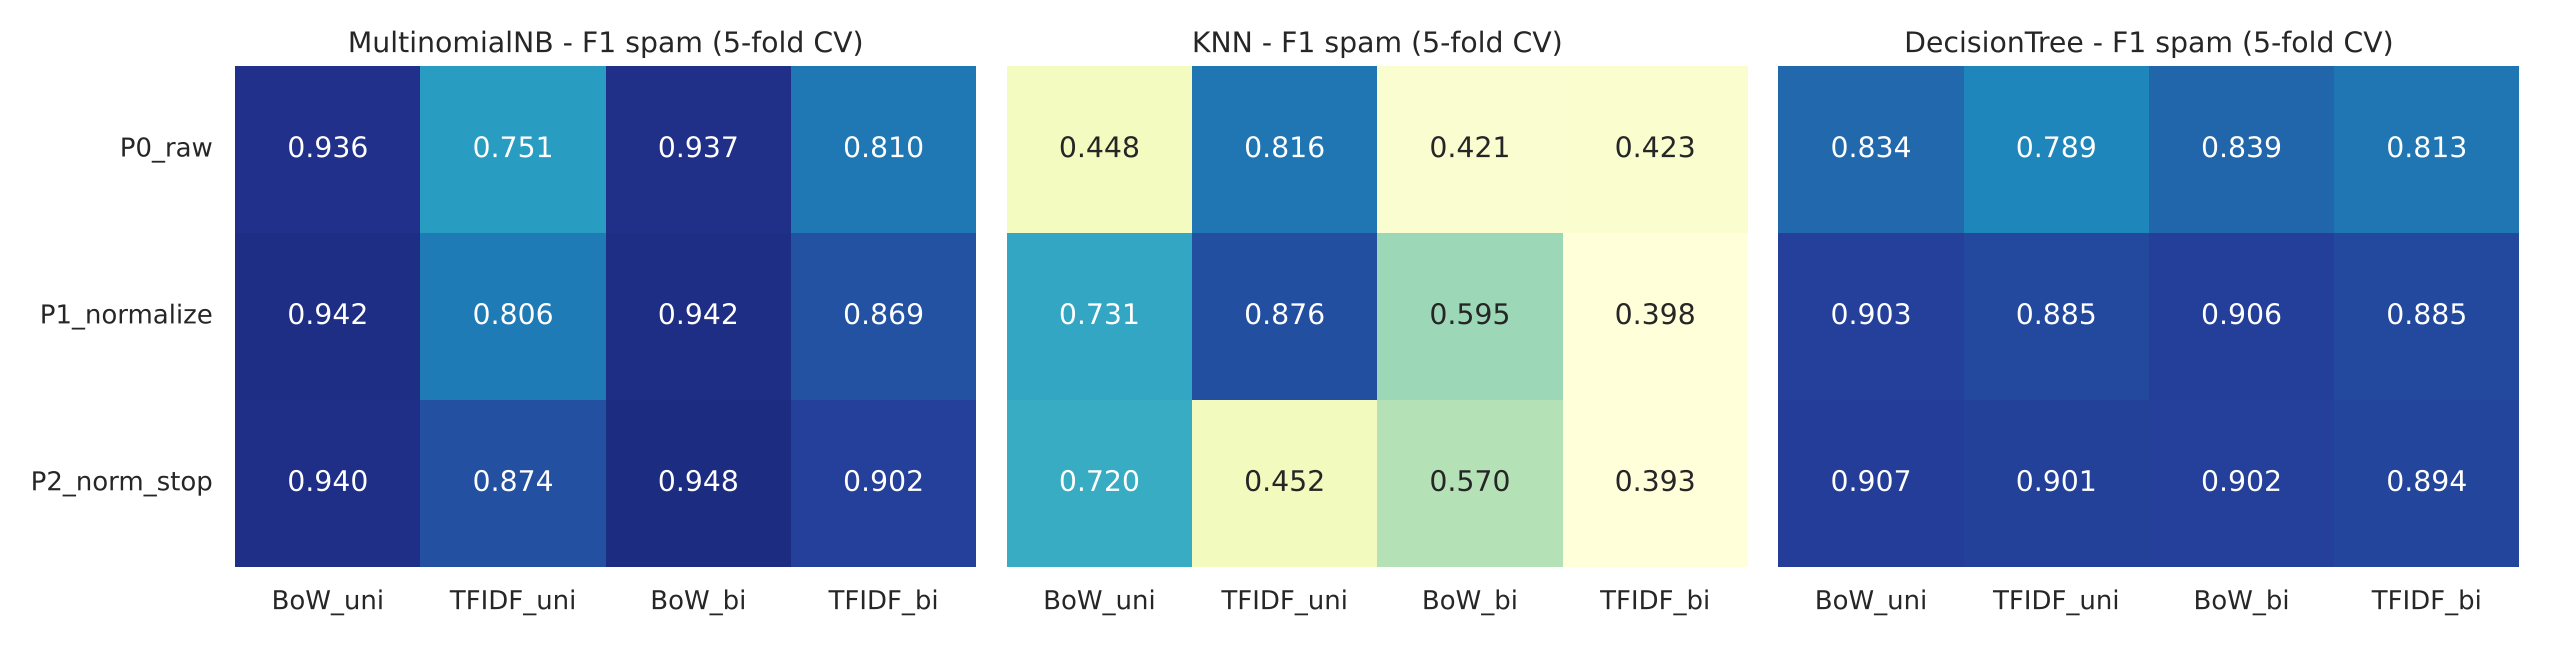
\includegraphics[width=\textwidth]{images/stage1_heatmap_cv_f1.png}
    \caption{Biểu đồ nhiệt so sánh điểm F1 lớp spam (5-fold CV) của 36 cấu hình thực nghiệm ở Giai đoạn 1 (siêu tham số mặc định)}
    \label{fig:stage1-heatmaps}
    \Nguon{Trích xuất tự động từ module run\_experiments.py}
\end{figure}

Phân tích Hình~\ref{fig:stage1-heatmaps} mang lại ba phát hiện quan trọng:
\begin{enumerate}
    \item \textbf{Tác động tích cực của tiền xử lý bảo toàn tín hiệu (P1 và P2):}
    Đối với Cây quyết định, việc chuyển từ tiền xử lý thô P0 sang P1 (bảo toàn tín hiệu regex) làm điểm F1 CV của cấu hình BoW unigram tăng vọt từ $0,834$ lên $0,903$ (tăng tới 6,9 điểm phần trăm), và tiếp tục đạt $0,907$ ở P2. Đối với Naive Bayes, F1 CV cũng tăng từ $0,936$ lên $0,942$. Điều này bước đầu kiểm chứng tính đúng đắn của Giả thuyết H1.
    \item \textbf{Nghịch lý TF-IDF trên Naive Bayes với $\alpha=1.0$ mặc định:}
    Trên biểu đồ của MultinomialNB, các ô sử dụng biểu diễn TF-IDF đều có điểm F1 rất thấp so với BoW. Cụ thể, ở mức tiền xử lý P0, BoW unigram đạt F1 là $0,936$ trong khi TF-IDF unigram chỉ đạt $0,751$ (giảm tới 18,5 điểm phần trăm). Tuy nhiên, nhóm không vội vàng kết luận TF-IDF kém hơn BoW, mà nghi vấn rằng chính hệ số làm trơn $\alpha=1.0$ mặc định đã bóp méo xác suất của các vector TF-IDF có độ lớn cực nhỏ.
    \item \textbf{Sự bất ổn định của K-NN:}
    Với khoảng cách Euclid mặc định, K-NN dao động dữ dội và có nhiều ô cấu hình F1 chỉ đạt dưới $0,400$.
\end{enumerate}

\section{Giai đoạn 2: Tinh chỉnh siêu tham số theo từng ô cấu hình}
\label{sec:giai-doan-2}

Bước sang Giai đoạn 2, nhóm triển khai kỹ thuật tinh chỉnh siêu tham số tối ưu bằng \texttt{GridSearchCV} 5-fold CV cho từng ô cấu hình của MultinomialNB và K-NN, sau đó đối sánh lại điểm F1 CV tối ưu giữa các ô.

Biểu đồ nhiệt kết quả F1 CV sau khi đã được tối ưu hóa siêu tham số được trình bày tại Hình~\ref{fig:stage2-heatmaps}.

\begin{figure}[H]
    \centering
    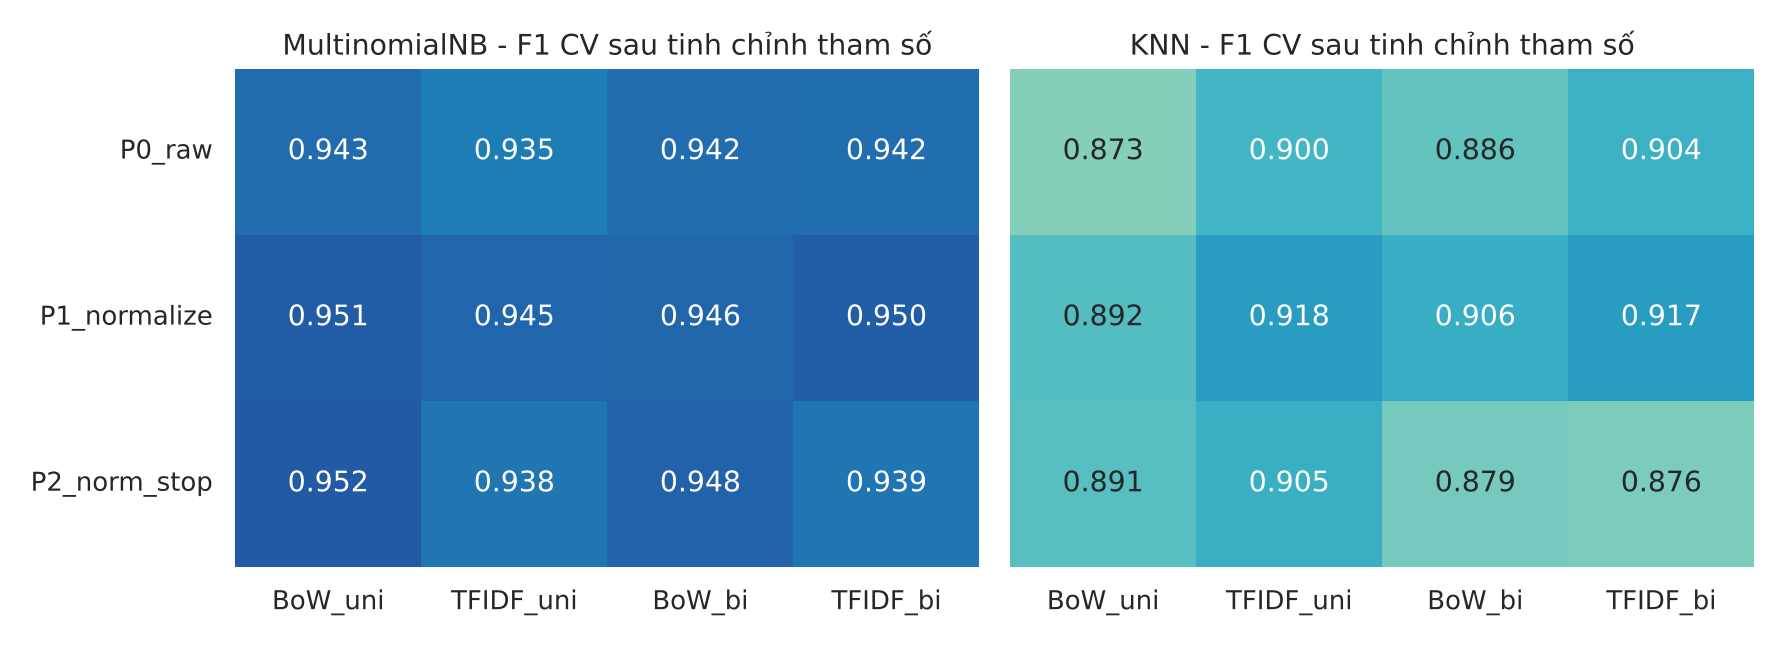
\includegraphics[width=0.88\textwidth]{images/stage2_heatmap_tuned_cv_f1.png}
    \caption{Biểu đồ nhiệt điểm F1 CV của MultinomialNB và K-NN sau khi đã tinh chỉnh siêu tham số tối ưu trong từng ô cấu hình}
    \label{fig:stage2-heatmaps}
    \Nguon{Trích xuất tự động từ module run\_experiments.py}
\end{figure}

\textbf{Phát hiện bước ngoặt từ Hình~\ref{fig:stage2-heatmaps}:}
\begin{itemize}
    \item Khi mỗi ô biểu diễn được trao cơ hội tìm kiếm siêu tham số $\alpha$ phù hợp với chính nó, khoảng cách hiệu năng giữa BoW và TF-IDF trên Naive Bayes đã \textbf{hoàn toàn biến mất}! Mọi ô cấu hình của Naive Bayes đều đạt điểm F1 CV xuất sắc trong dải rất hẹp từ $0,935$ đến $0,952$. Điều này chứng minh giả thuyết phương pháp luận của nhóm là hoàn toàn chính xác: TF-IDF ở Giai đoạn 1 bị điểm thấp thuần túy là do tham số $\alpha=1.0$ mặc định không tương thích, chứ không phải do bản chất của phép biểu diễn TF-IDF!
    \item Đối với K-NN, khi được chuyển sang khoảng cách \texttt{cosine}, trọng số \texttt{distance} và $K=9$, điểm F1 CV của cấu hình P1 + TF-IDF unigram đã tăng vọt từ $0,876$ lên \textbf{$0,918$}, đưa K-NN trở thành một bộ phân loại có hiệu năng cạnh tranh sòng phẳng với Cây quyết định.
\end{itemize}

Dựa trên kết quả F1 thẩm định chéo 5-fold CV cao nhất trên tập huấn luyện, cấu hình tối ưu cuối cùng được lựa chọn cho mỗi thuật toán được tổng hợp trong Bảng~\ref{tab:cau-hinh-toi-uu}.

\begin{table}[H]
\centering
\caption{Cấu hình tối ưu được lựa chọn cho từng mô hình dựa trên 5-fold CV tập huấn luyện}
\label{tab:cau-hinh-toi-uu}
\begin{tabular}{|l|c|c|p{4.2cm}|c|c|}
\hline
\textbf{Mô hình} & \textbf{Tiền xử lý} & \textbf{Biểu diễn} & \textbf{Siêu tham số tối ưu} & \textbf{CV-F1 mặc định} & \textbf{CV-F1 tinh chỉnh} \\
\hline
\textbf{MultinomialNB} & P2\_norm\_stop & BoW\_uni & $\alpha=2.0$, \texttt{fit\_prior=True} & 0,9400 & \textbf{0,9518} \\
\hline
\textbf{K-NN} & P1\_normalize & TFIDF\_uni & \texttt{metric='cosine'}, $K=9$, \texttt{weights='distance'} & 0,8759 & \textbf{0,9176} \\
\hline
\textbf{DecisionTree} & P2\_norm\_stop & BoW\_uni & \texttt{criterion='gini'}, \texttt{max\_depth=10}, \texttt{min\_samples\_leaf=1} & 0,9072 & \textbf{0,9110} \\
\hline
\end{tabular}
\Nguon{Trích xuất tự động từ results/summary.json}
\end{table}

\subsection{Phân tích đường cong siêu tham số}
Hình~\ref{fig:param-curves} mô tả trực quan sự biến thiên của điểm F1 CV theo các siêu tham số đơn lẻ quan trọng nhất của từng mô hình (khi các tham số còn lại được cố định tại giá trị tối ưu).

\begin{figure}[H]
    \centering
    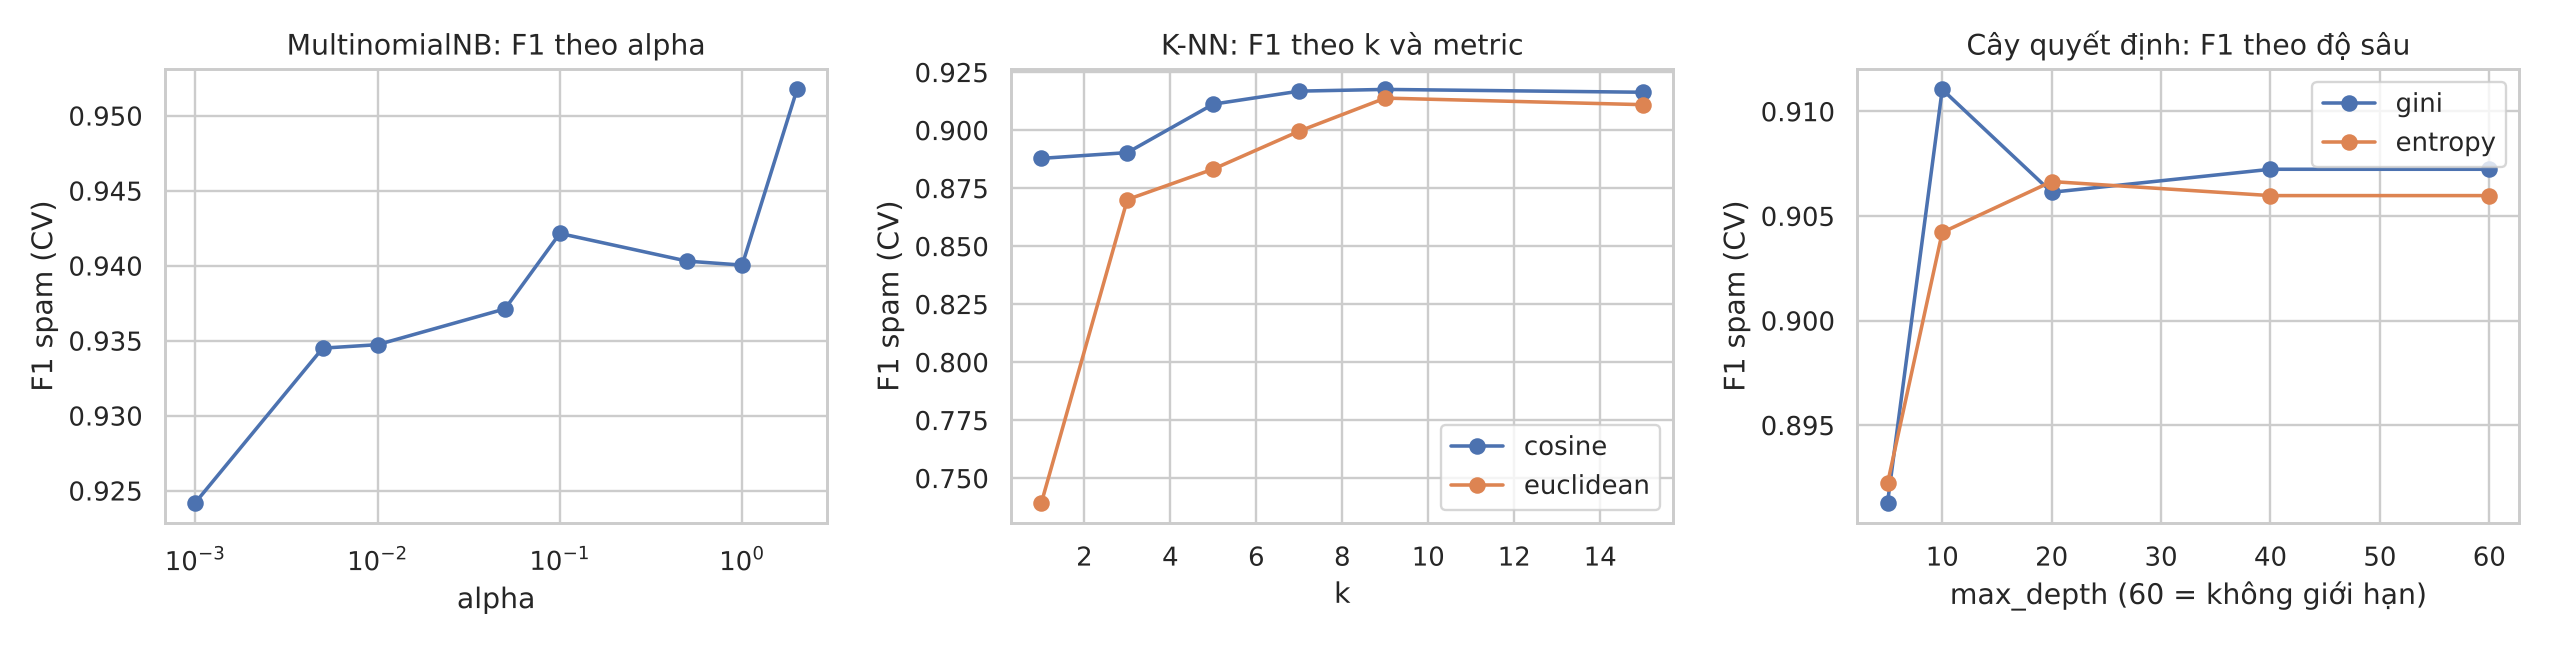
\includegraphics[width=\textwidth]{images/stage2_param_curves.png}
    \caption{Đường cong biến thiên điểm F1 CV theo siêu tham số chính: MultinomialNB theo $\alpha$ (trái), K-NN theo $K$ và metric (giữa), Cây quyết định theo độ sâu \texttt{max\_depth} (phải)}
    \label{fig:param-curves}
    \Nguon{Trích xuất tự động từ module run\_experiments.py}
\end{figure}

\begin{enumerate}
    \item \textbf{MultinomialNB theo $\alpha$ (Hình trái):} Điểm F1 CV tăng dần đều từ vùng $\alpha = 0.001$ và đạt đỉnh cực đại tại $\alpha = 2.0$. Do điểm cực đại nằm ở cận trên của lưới ban đầu, nhóm đã triển khai thêm thực nghiệm mở rộng ở Mục~\ref{sec:mo-rong-alpha}.
    \item \textbf{K-NN theo $K$ và hàm khoảng cách (Hình giữa):} Khoảng cách \texttt{cosine} thể hiện sự vượt trội hoàn toàn so với \texttt{euclidean} tại mọi giá trị $K$. Đường cong F1 của \texttt{cosine} tăng nhanh từ $K=1$ đến $K=7$ và đi vào vùng bão hòa ổn định ở $K=7, 9, 15$. Giá trị $K=9$ được lựa chọn vì mang lại sự cân bằng tốt nhất giữa độ mịn của ranh giới quyết định và khả năng kháng nhiễu.
    \item \textbf{Cây quyết định theo \texttt{max\_depth} (Hình phải):} Tiêu chí \texttt{gini} mang lại hiệu năng nhỉnh hơn tiêu chí \texttt{entropy}. Đường cong F1 đạt đỉnh rõ nét tại độ sâu \texttt{max\_depth=10} ($F_1 = 0,9110$). Khi tăng độ sâu lên $20, 40$ hoặc không giới hạn (\texttt{None}), điểm F1 giảm dần do hiện tượng quá khớp (Overfitting) trên các từ vựng cá biệt.
\end{enumerate}

\section{Thực nghiệm mở rộng: Khảo sát độ nhạy tham số làm trơn $\alpha$ của Naive Bayes}
\label{sec:mo-rong-alpha}

Do trong lưới tìm kiếm ban đầu, $\alpha = 2.0$ là giá trị lớn nhất được khảo sát và đạt điểm F1 cao nhất, một câu hỏi khoa học quan trọng được đặt ra: *“Nếu tiếp tục tăng $\alpha$ lên các giá trị lớn hơn ($3, 5, 10$), liệu hiệu năng của Naive Bayes có tiếp tục tăng hay không?”*.

Để trả lời câu hỏi này, nhóm đã xây dựng module độc lập \texttt{src/extra\_nb\_alpha\_check.py}, mở rộng dải khảo sát $\alpha \in [0.1, 0.5, 1, 2, 3, 5, 10]$ và lặp lại trên 3 seed phân chia fold thẩm định chéo khác nhau để triệt tiêu nhiễu ngẫu nhiên. Kết quả trung bình được tổng hợp tại Bảng~\ref{tab:nb-alpha-sensitivity}.

\begin{table}[H]
\centering
\caption{Khảo sát độ nhạy của Multinomial Naive Bayes theo tham số làm trơn $\alpha$ (trung bình qua 3 seed phân chia fold)}
\label{tab:nb-alpha-sensitivity}
\begin{tabular}{|c|c|c|c|l|}
\hline
\textbf{Hệ số $\alpha$} & \textbf{F1-Score} & \textbf{Precision} & \textbf{Recall} & \textbf{Nhận xét xu hướng} \\
\hline
0,1 & 0,9396 & 0,9314 & 0,9483 & Mô hình nhạy, dễ báo động nhầm \\
\hline
0,5 & 0,9390 & 0,9278 & 0,9508 & Recall cao, Precision thấp \\
\hline
1,0 & 0,9396 & 0,9315 & 0,9483 & Làm trơn Laplace chuẩn \\
\hline
\textbf{2,0} & \textbf{0,9503} & \textbf{0,9541} & \textbf{0,9470} & \textbf{Điểm cân bằng tối ưu toàn cục} \\
\hline
3,0 & 0,9488 & 0,9622 & 0,9361 & Precision tăng, Recall bắt đầu giảm \\
\hline
5,0 & 0,9460 & 0,9725 & 0,9214 & Bắt đầu bỏ sót nhiều tin rác \\
\hline
10,0 & 0,9409 & 0,9826 & 0,9029 & Precision rất cao nhưng Recall tụt sâu \\
\hline
\end{tabular}
\Nguon{Trích xuất tự động từ module extra\_nb\_alpha\_check.py}
\end{table}

\textbf{Quy luật đánh đổi sâu sắc:}
Số liệu tại Bảng~\ref{tab:nb-alpha-sensitivity} đã làm sáng tỏ bản chất toán học của hệ số làm trơn $\alpha$:
\begin{itemize}
    \item Khi $\alpha$ càng lớn, xác suất có điều kiện $\hat{P}(w_i|y)$ càng bị kéo mạnh về phía phân phối đều $\frac{1}{|\mathcal{V}|}$. Mô hình trở nên "thận trọng" và dè dặt hơn rất nhiều khi gán nhãn spam cho một tin nhắn.
    \item Do đó, khi $\alpha$ tăng từ $2.0$ lên $10.0$, chỉ số Precision tăng vọt từ $95,41\%$ lên tới \textbf{$98,26\%$} (hầu như không bao giờ chặn nhầm tin hợp lệ), nhưng phải trả giá bằng việc chỉ số Recall tụt giảm từ $94,70\%$ xuống \textbf{$90,29\%$} (bỏ lọt nhiều tin rác hơn).
    \item Điểm số F1-score đạt đỉnh thực sự tại $\alpha = 2.0$ ($F_1 = 0,9503$) và bắt đầu suy giảm đơn điệu khi $\alpha > 2.0$. Thực nghiệm này chứng minh trọn vẹn rằng $\alpha = 2.0$ là điểm tối ưu toàn cục đích thực.
\end{itemize}

\section{Thực nghiệm có kiểm soát về các tham số của Vectorizer}
\label{sec:thuc-nghiem-vectorizer}

Để đáp ứng toàn diện yêu cầu tại Mục 3.1 trong tài liệu hướng dẫn bài tập lớn của học phần (khảo sát ảnh hưởng của n-gram, \texttt{min\_df}, \texttt{max\_df} và số lượng đặc trưng), nhóm đã tiến hành một thực nghiệm có kiểm soát nghiêm ngặt thông qua module \texttt{src/vectorizer\_sensitivity.py}. Đối với mỗi mô hình, nhóm giữ nguyên tiền xử lý, loại biểu diễn và siêu tham số tối ưu đã chọn ở Bảng~\ref{tab:cau-hinh-toi-uu}, chỉ thay đổi độc lập từng tham số vector hóa trên tập huấn luyện (5-fold CV).

\begin{figure}[H]
    \centering
    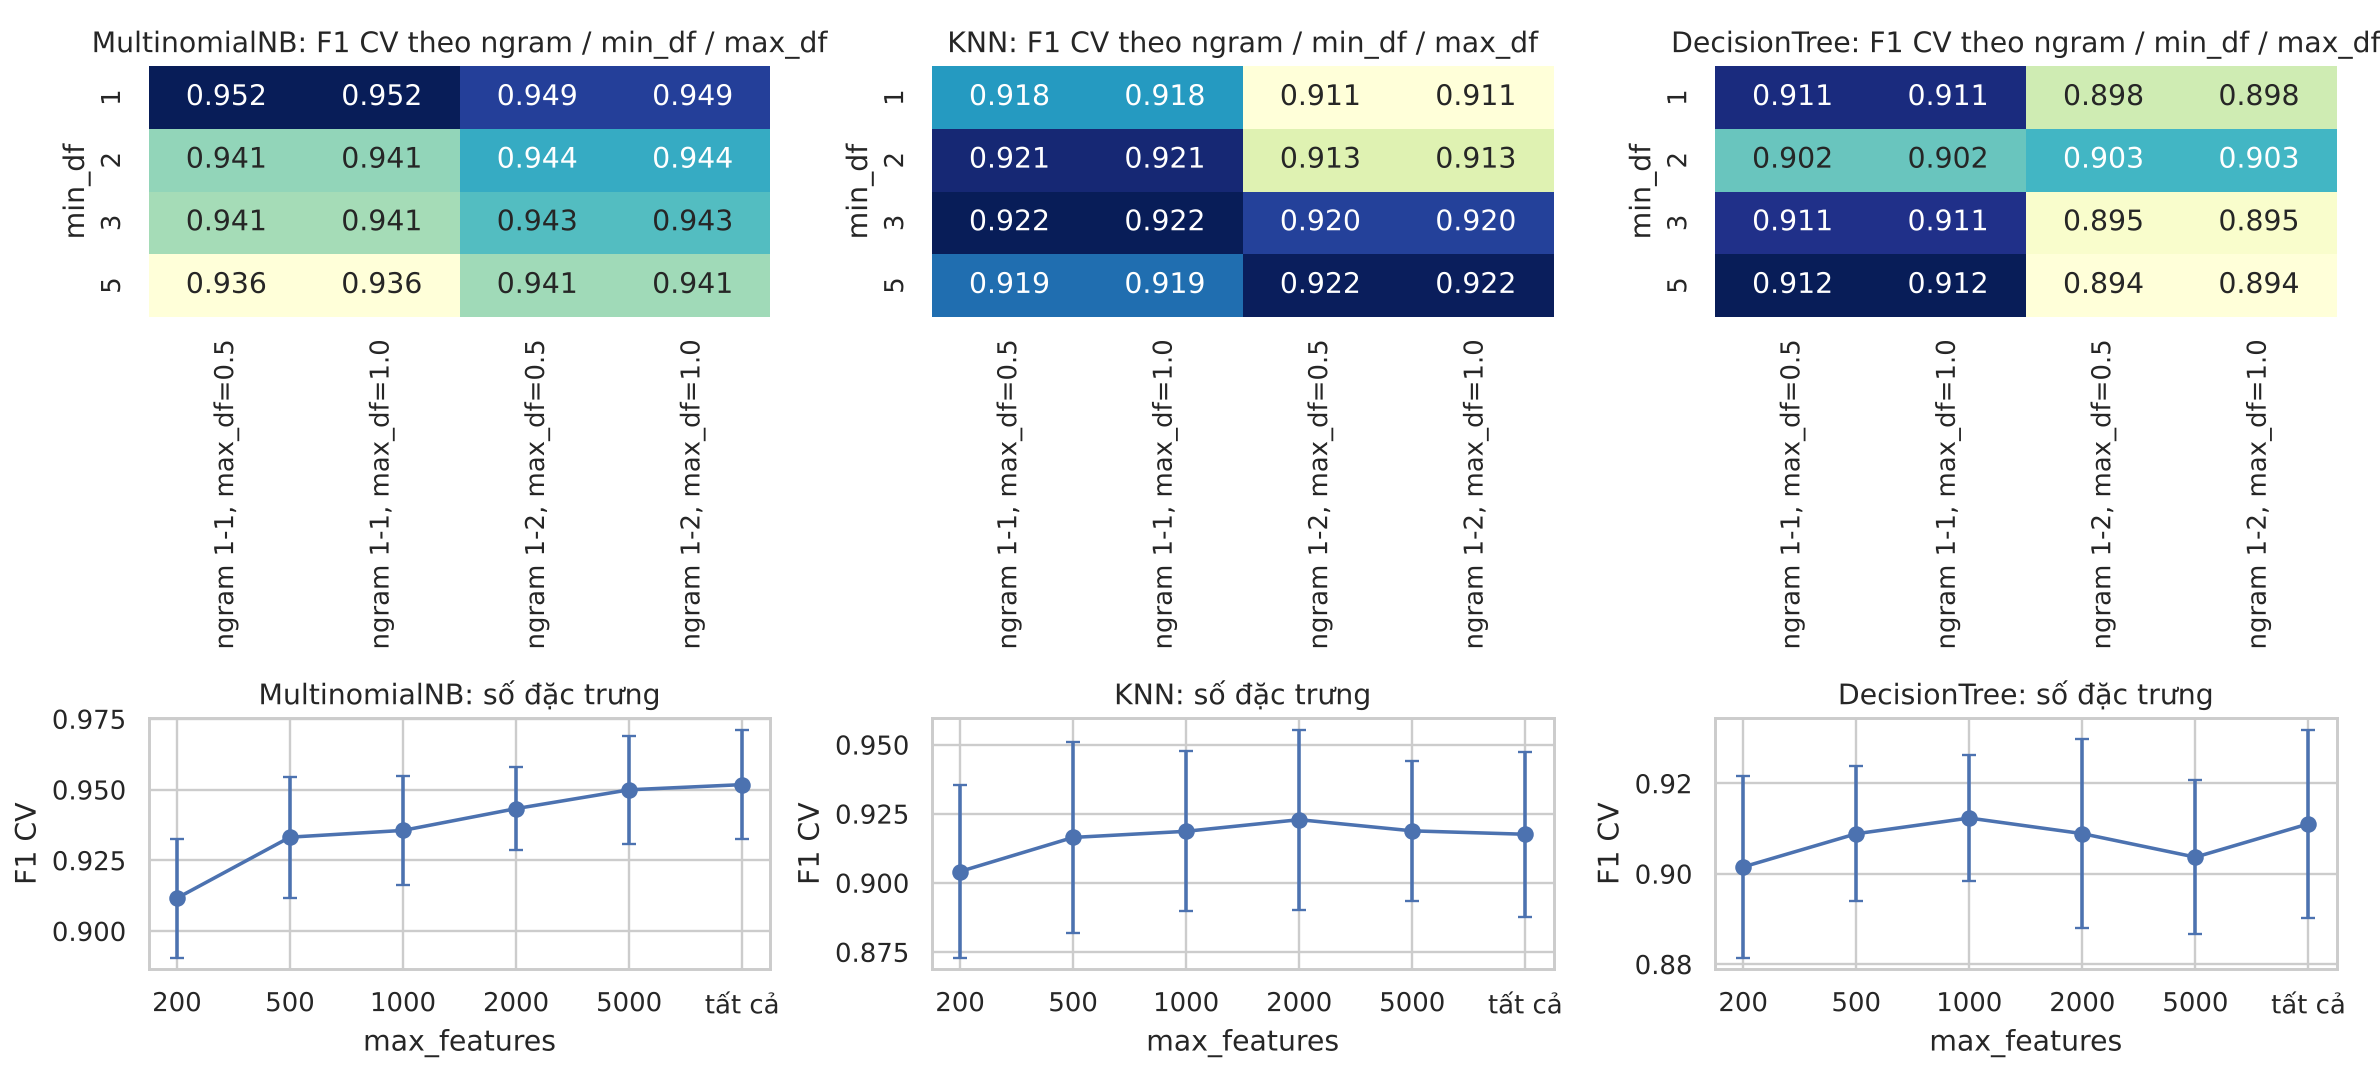
\includegraphics[width=\textwidth]{images/vectorizer_sensitivity.png}
    \caption{Thực nghiệm có kiểm soát về tham số Vectorizer: Lưới n-gram $\times$ \texttt{min\_df} $\times$ \texttt{max\_df} (hàng trên) và đường cong F1 theo số lượng đặc trưng \texttt{max\_features} (hàng dưới)}
    \label{fig:vectorizer-sensitivity}
    \Nguon{Trích xuất tự động từ module vectorizer\_sensitivity.py}
\end{figure}

\subsection{Khảo sát tương tác n-gram, \texttt{min\_df} và \texttt{max\_df}}
Bảng~\ref{tab:vectorizer-grid} trình bày chi tiết điểm F1 CV của 3 mô hình khi thay đổi bậc n-gram và ngưỡng tần số tài liệu tối thiểu \texttt{min\_df} (khi \texttt{max\_df=1.0}).

\begin{table}[H]
\centering
\caption{F1 CV theo bậc n-gram và ngưỡng min\_df (với max\_df=1.0)}
\label{tab:vectorizer-grid}
\begin{tabular}{|l|l|c|c|c|c|}
\hline
\textbf{Mô hình} & \textbf{Biểu diễn n-gram} & \textbf{min\_df=1} & \textbf{min\_df=2} & \textbf{min\_df=3} & \textbf{min\_df=5} \\
\hline
\multirow{2}{*}{\textbf{MultinomialNB}} & unigram (1-1) & \textbf{0,9518} & 0,9412 & 0,9407 & 0,9357 \\
\cline{2-6}
& unigram + bigram (1-2) & 0,9492 & 0,9443 & 0,9432 & 0,9408 \\
\hline
\multirow{2}{*}{\textbf{K-NN}} & unigram (1-1) & 0,9176 & 0,9213 & \textbf{0,9219} & 0,9188 \\
\cline{2-6}
& unigram + bigram (1-2) & 0,9112 & 0,9130 & 0,9201 & 0,9218 \\
\hline
\multirow{2}{*}{\textbf{DecisionTree}} & unigram (1-1) & 0,9110 & 0,9020 & 0,9106 & \textbf{0,9125} \\
\cline{2-6}
& unigram + bigram (1-2) & 0,8985 & 0,9034 & 0,8952 & 0,8944 \\
\hline
\end{tabular}
\Nguon{Trích xuất tự động từ results/vectorizer\_sensitivity.csv}
\end{table}

\textbf{Các quan sát thực nghiệm cốt lõi:}
\begin{enumerate}
    \item \textbf{Về tham số \texttt{max\_df}:} Khi chuyển từ \texttt{max\_df=1.0} sang \texttt{max\_df=0.5}, kết quả F1 CV của toàn bộ các ô ở cả ba mô hình \textbf{hoàn toàn giống hệt nhau} (sai số $0.0000$). Điều này chứng minh rằng trong tập dữ liệu SMS Spam, không có bất kỳ từ khóa nào xuất hiện trong hơn 50\% tổng số tin nhắn. Do đó, tham số \texttt{max\_df} không có tác động thực tế trong bài toán này.
    \item \textbf{Về vai trò của Bigram và kiểm chứng Giả thuyết H2:} Khi so sánh công bằng ở cùng ngưỡng \texttt{min\_df=2}, mô hình kết hợp unigram + bigram của Naive Bayes đạt F1 là $0,9443$, chỉ nhỉnh hơn unigram ($0,9412$) một lượng rất nhỏ $0,0031$. Tuy nhiên, độ lệch chuẩn F1 giữa các fold của Naive Bayes là $\approx 0,017$. Do mức chênh lệch nhỏ hơn nhiều so với độ lệch chuẩn, \textbf{Giả thuyết H2 không được dữ liệu thực nghiệm ủng hộ}. Trong các tin nhắn SMS rất ngắn, các cụm hai từ hiếm khi lặp lại đủ nhiều để tạo ra sự đột phá ngữ nghĩa so với các từ đơn lẻ.
    \item \textbf{Về ngưỡng \texttt{min\_df}:} Việc tăng \texttt{min\_df} từ 1 lên 5 giúp loại bỏ hàng nghìn từ hiếm, giảm kích thước từ vựng nhưng làm điểm F1 của Naive Bayes giảm nhẹ từ $0,9518$ xuống $0,9357$.
\end{enumerate}

\subsection{Khảo sát giới hạn số lượng đặc trưng (\texttt{max\_features})}
Bảng~\ref{tab:max-features-study} thể hiện sự biến thiên của F1 CV khi giới hạn kích thước từ vựng tối đa từ 200 từ đến toàn bộ từ điển ($\approx 6.500$ từ).

\begin{table}[H]
\centering
\caption{F1 CV theo số lượng đặc trưng tối đa max\_features (unigram, min\_df=1)}
\label{tab:max-features-study}
\begin{tabular}{|l|c|c|c|c|c|c|}
\hline
\textbf{Mô hình} & \textbf{200 từ} & \textbf{500 từ} & \textbf{1.000 từ} & \textbf{2.000 từ} & \textbf{5.000 từ} & \textbf{Tất cả ($\approx$6.500)} \\
\hline
MultinomialNB & 0,9116 & 0,9332 & 0,9356 & 0,9433 & 0,9499 & \textbf{0,9518} \\
\hline
K-NN & 0,9041 & 0,9164 & 0,9187 & \textbf{0,9229} & 0,9188 & 0,9176 \\
\hline
DecisionTree & 0,9015 & 0,9089 & \textbf{0,9123} & 0,9089 & 0,9037 & 0,9110 \\
\hline
\end{tabular}
\Nguon{Trích xuất tự động từ results/vectorizer\_sensitivity.csv}
\end{table}

Từ Bảng~\ref{tab:max-features-study} và biểu đồ hàng dưới tại Hình~\ref{fig:vectorizer-sensitivity}:
\begin{itemize}
    \item Chỉ khi cắt giảm từ điển xuống mức cực đoan (200 từ), hiệu năng mô hình mới bị suy giảm rõ rệt (F1 của Naive Bayes giảm từ $0,9518$ xuống $0,9116$, mức giảm gấp 2 lần độ lệch chuẩn).
    \item Từ ngưỡng \textbf{2.000 từ} trở lên, hiệu năng của cả 3 mô hình đã tiệm cận mức tối đa và đi vào vùng bão hòa hoàn toàn.
    \item Với tài nguyên tính toán hiện đại, việc lưu trữ 6.500 đặc trưng là hoàn toàn khả thi và không gây áp lực bộ nhớ, do đó giữ lại toàn bộ từ vựng là giải pháp tối ưu.
\end{itemize}

\section{Đánh giá tổng hợp trên tập kiểm thử độc lập (Test Set)}
\label{sec:danh-gia-test}

Sau khi đã xác định được cấu hình tối ưu nhất cho từng thuật toán thông qua quy trình thẩm định chéo nghiêm ngặt trên tập huấn luyện, toàn bộ 3 mô hình được huấn luyện lại trên toàn bộ 4.136 mẫu của tập Train và được đánh giá một lần duy nhất trên tập kiểm thử độc lập gồm 1.035 mẫu (trong đó có 131 mẫu tin nhắn rác).

\subsection{Đối sánh toàn diện Baseline và Mô hình tinh chỉnh}
Bảng~\ref{tab:baseline-vs-tuned} đối sánh chi tiết sự cải thiện của từng chỉ số giữa phương án Baseline ban đầu và mô hình sau tinh chỉnh tối ưu.

\begin{table}[H]
\centering
\caption{Đối sánh hiệu năng giữa phương án Baseline và Cấu hình tinh chỉnh trên tập kiểm thử}
\label{tab:baseline-vs-tuned}
\begin{tabular}{|l|l|c|c|c|c|}
\hline
\textbf{Thuật toán} & \textbf{Phương án} & \textbf{Accuracy} & \textbf{Precision} & \textbf{Recall} & \textbf{F1-Score} \\
\hline
\multirow{2}{*}{\textbf{Multinomial NB}} & Baseline & 0,9807 & 0,9512 & 0,8931 & 0,9213 \\
\cline{2-6}
& Tinh chỉnh & \textbf{0,9913} & \textbf{0,9766} & \textbf{0,9542} & \textbf{0,9653} \\
\hline
\multirow{2}{*}{\textbf{K-NN}} & Baseline & 0,9072 & 1,0000 & 0,2672 & 0,4217 \\
\cline{2-6}
& Tinh chỉnh & \textbf{0,9826} & \textbf{0,9593} & \textbf{0,9008} & \textbf{0,9291} \\
\hline
\multirow{2}{*}{\textbf{Decision Tree}} & Baseline & 0,9691 & 0,9024 & 0,8473 & 0,8740 \\
\cline{2-6}
& Tinh chỉnh & \textbf{0,9874} & \textbf{1,0000} & \textbf{0,9008} & \textbf{0,9478} \\
\hline
\end{tabular}
\Nguon{Trích xuất từ results/baseline\_vs\_tuned.csv}
\end{table}

Kết quả ở Bảng~\ref{tab:baseline-vs-tuned} chứng minh sự tiến bộ vượt bậc của toàn bộ các mô hình sau khi được tối ưu hóa:
\begin{itemize}
    \item Multinomial Naive Bayes nâng F1 từ $0,9213$ lên \textbf{$0,9653$} (Recall tăng ấn tượng từ $89,31\%$ lên $95,42\%$).
    \item K-NN tạo ra bước nhảy vọt ngoạn mục nhất: F1 tăng từ $0,4217$ lên \textbf{$0,9291$} (Recall tăng từ $26,72\%$ lên $90,08\%$, khắc phục hoàn toàn nhược điểm bỏ sót tin rác).
    \item Cây quyết định nâng F1 từ $0,8740$ lên \textbf{$0,9478$}, đặc biệt đạt được chỉ số \textbf{Precision tuyệt đối $100\%$} (không chặn nhầm bất kỳ tin nhắn hợp lệ nào trên tập test).
\end{itemize}

\subsection{Bảng chỉ số đánh giá cuối cùng}
Bảng~\ref{tab:ket-qua-cuoi-cung} tổng hợp toàn bộ các chỉ số kiểm thử cuối cùng cùng số lượng lỗi thực tế tương ứng của 3 mô hình.

\begin{table}[H]
\centering
\caption{Kết quả đánh giá kiểm thử cuối cùng trên tập Test (1.035 tin nhắn, 131 spam)}
\label{tab:ket-qua-cuoi-cung}
\begin{tabular}{|l|c|c|c|c|c|c|}
\hline
\textbf{Mô hình tối ưu} & \textbf{Accuracy} & \textbf{Precision} & \textbf{Recall} & \textbf{F1-Score} & \textbf{ROC-AUC} & \textbf{Số lỗi (FP / FN)} \\
\hline
\textbf{Multinomial NB} & \textbf{0,9913} & 0,9766 & \textbf{0,9542} & \textbf{0,9653} & 0,9860 & \textbf{3 / 6 (Tổng: 9)} \\
\hline
\textbf{K-NN} & 0,9826 & 0,9593 & 0,9008 & 0,9291 & \textbf{0,9919} & 5 / 13 (Tổng: 18) \\
\hline
\textbf{Decision Tree} & 0,9874 & \textbf{1,0000} & 0,9008 & 0,9478 & 0,9500 & \textbf{0 / 13 (Tổng: 13)} \\
\hline
\end{tabular}
\Nguon{Trích xuất từ results/final\_test\_results.csv và summary.json}
\end{table}

\subsection{Trực quan hóa Ma trận nhầm lẫn và Đường cong ROC}
Hình~\ref{fig:confusion-matrices} thể hiện ma trận nhầm lẫn trực quan của 3 mô hình trên tập kiểm thử 1.035 mẫu.

\begin{figure}[H]
    \centering
    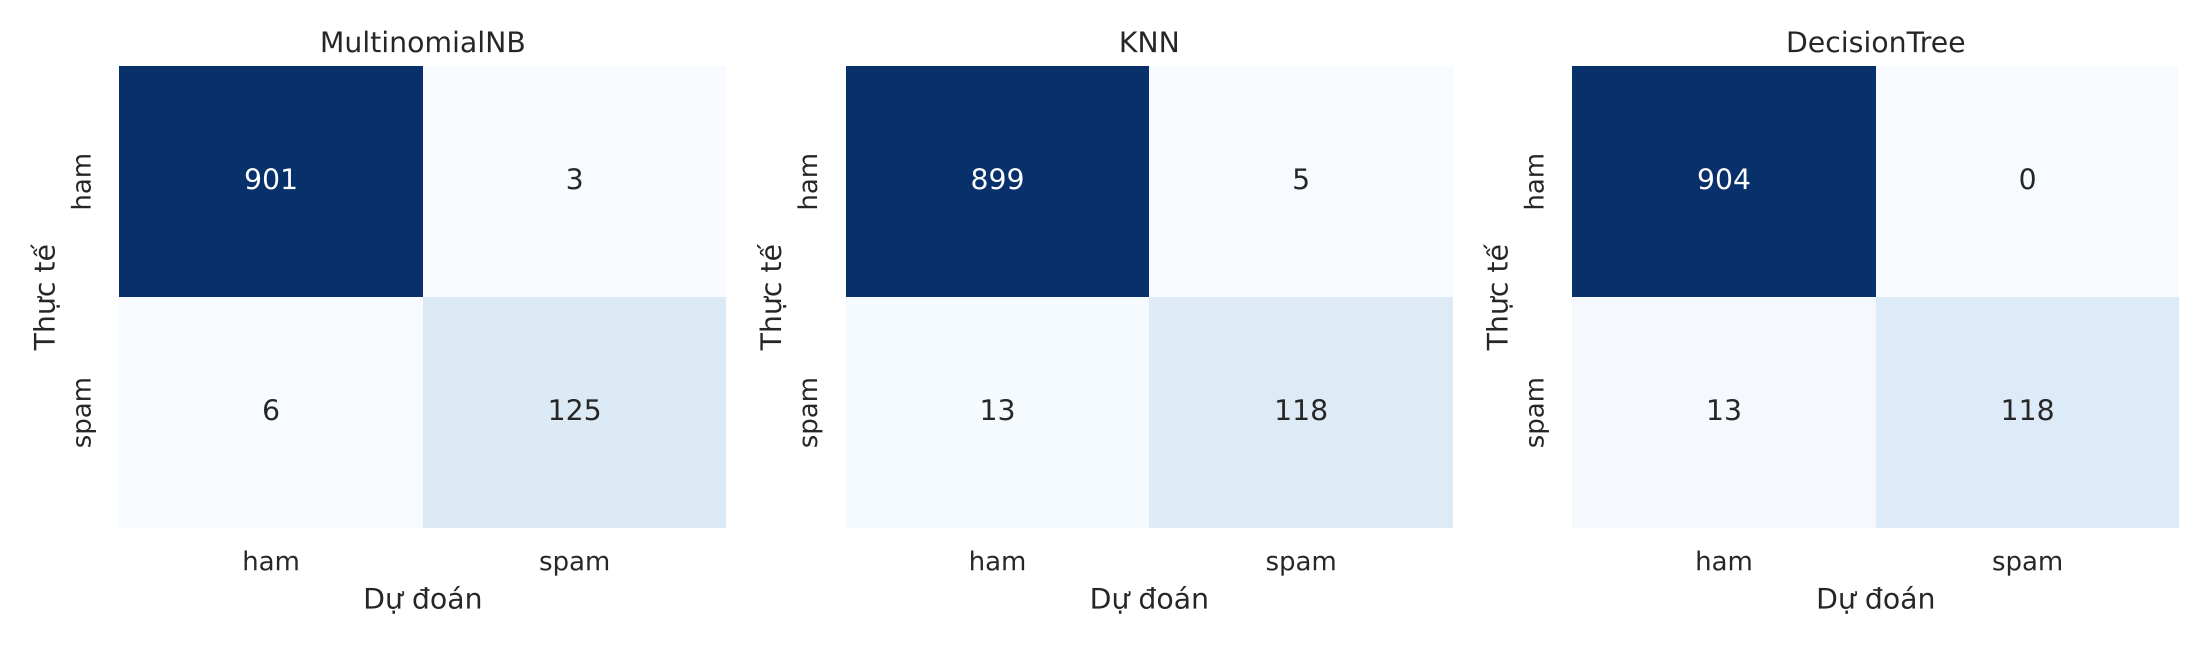
\includegraphics[width=\textwidth]{images/confusion_matrices.png}
    \caption{Ma trận nhầm lẫn của 3 mô hình tối ưu trên tập kiểm thử (1.035 tin nhắn)}
    \label{fig:confusion-matrices}
    \Nguon{Trích xuất tự động từ module run\_experiments.py}
\end{figure}

Từ ma trận nhầm lẫn tại Hình~\ref{fig:confusion-matrices}:
\begin{itemize}
    \item \textbf{MultinomialNB:} Dự đoán chính xác 901/904 tin hợp lệ và 125/131 tin nhắn rác. Chỉ có đúng 3 trường hợp báo nhầm (FP) và 6 trường hợp bỏ sót (FN), đạt tổng số lỗi thấp nhất toàn hệ thống (9 lỗi / 1.035 tin).
    \item \textbf{K-NN:} Dự đoán chính xác 899/904 tin hợp lệ và 118/131 tin rác. Có 5 trường hợp báo nhầm (FP) và 13 trường hợp bỏ sót (FN).
    \item \textbf{Decision Tree:} Đạt thành tích đặc biệt khi dự đoán hoàn hảo 904/904 tin hợp lệ ($0$ trường hợp báo nhầm FP), nhưng bỏ sót 13 tin nhắn rác (FN).
\end{itemize}

\begin{figure}[H]
    \centering
    \begin{minipage}{0.48\textwidth}
        \centering
        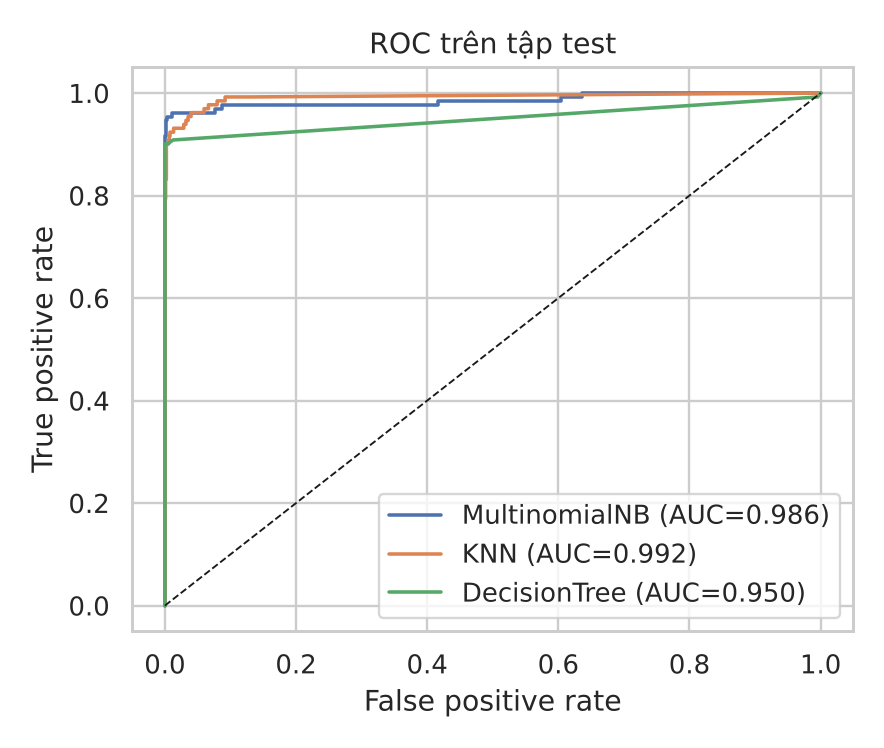
\includegraphics[width=\textwidth]{images/roc_curves.png}
        \caption*{(a) Đường cong ROC trên tập kiểm thử}
    \end{minipage}
    \hfill
    \begin{minipage}{0.50\textwidth}
        \centering
        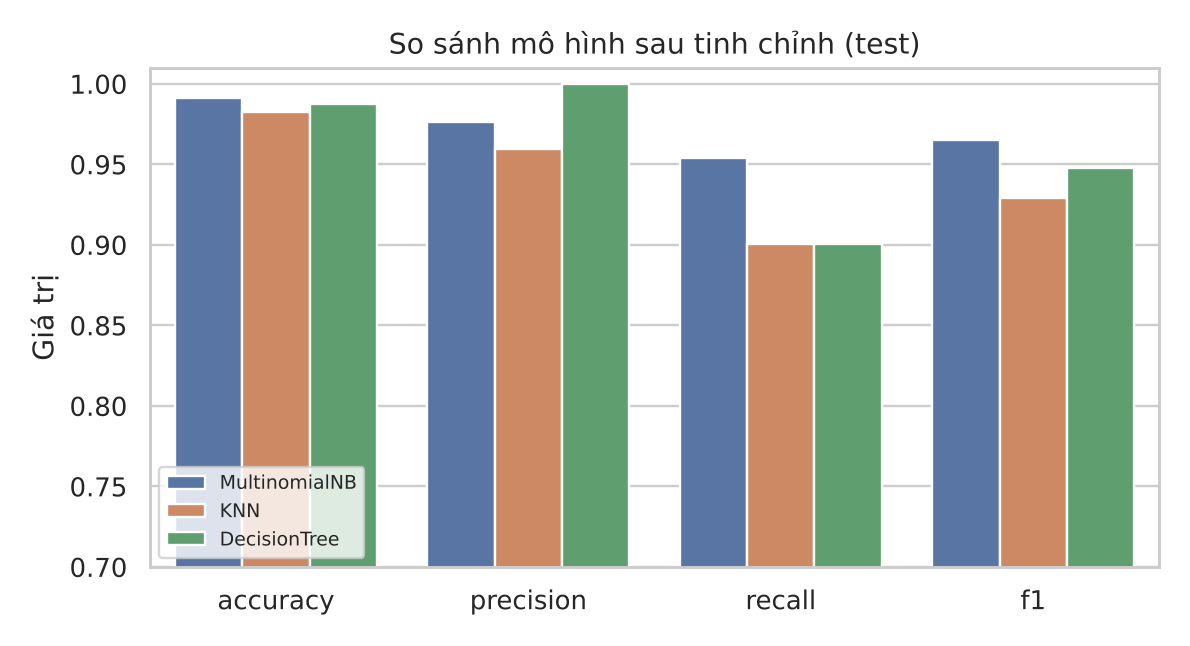
\includegraphics[width=\textwidth]{images/final_metric_bars.png}
        \caption*{(b) Biểu đồ cột đối sánh các độ đo}
    \end{minipage}
    \caption{Đường cong ROC và biểu đồ cột đối sánh các chỉ số hiệu năng của 3 mô hình tối ưu}
    \label{fig:roc-and-bars}
    \Nguon{Trích xuất tự động từ module run\_experiments.py}
\end{figure}

Hình~\ref{fig:roc-and-bars}a thể hiện đường cong ROC của cả 3 mô hình đều áp sát góc trên bên trái, minh chứng cho năng lực phân loại vượt trội. Đáng chú ý, mô hình \textbf{K-NN đạt chỉ số ROC-AUC cao nhất hệ thống lên tới $0,9919$}, vượt qua cả Naive Bayes ($0,9860$) và Cây quyết định ($0,9500$). Điều này chứng tỏ K-NN có khả năng xếp hạng xác suất (Probability Ranking) cực tốt; lý do điểm F1 của K-NN thấp hơn Naive Bayes là do ngưỡng cắt xác suất mặc định $\tau = 0.5$ chưa phải là ngưỡng tối ưu nhất đối với lớp thiểu số.

\section{Phân tích độ ổn định qua 5 lần phân chia ngẫu nhiên (5-Seed Stability Analysis)}
\label{sec:do-on-dinh-seed}

Một điểm yếu cố hữu của việc đánh giá mô hình chỉ trên một lần phân chia Train/Test duy nhất là sự phụ thuộc vào tính ngẫu nhiên: tập kiểm thử chỉ chứa 131 mẫu tin nhắn rác, do đó việc sai khác chỉ 1 tin nhắn spam duy nhất đã làm thay đổi chỉ số Recall tới gần \textbf{$0,8$ điểm phần trăm} ($\frac{1}{131} \approx 0,763\%$).

Để kiểm chứng tính vững chắc (Robustness) và loại bỏ yếu tố may rủi của một lần chia dữ liệu cụ thể, nhóm đã tiến hành thực nghiệm kiểm tra độ ổn định: giữ cố định toàn bộ siêu tham số tối ưu đã chọn ở Bảng~\ref{tab:cau-hinh-toi-uu}, lặp lại quy trình phân chia Stratified 80/20 trên \textbf{5 giá trị mầm ngẫu nhiên khác nhau} (\texttt{random\_state} $\in \{0, 1, 2, 3, 4\}$). Kết quả trung bình và độ lệch chuẩn ($\text{Mean} \pm \text{Std}$) được tổng hợp tại Bảng~\ref{tab:seed-stability}.

\begin{table}[H]
\centering
\caption{Độ ổn định hiệu năng của các mô hình qua 5 lần phân chia Train/Test khác nhau}
\label{tab:seed-stability}
\begin{tabular}{|l|c|c|c|c|c|}
\hline
\textbf{Mô hình} & \textbf{Accuracy} & \textbf{Precision} & \textbf{Recall} & \textbf{F1-Score} & \textbf{ROC-AUC} \\
\hline
\textbf{MultinomialNB} & $0,9865 \pm 0,0050$ & $0,9470 \pm 0,0280$ & $\mathbf{0,9466 \pm 0,0179}$ & $\mathbf{0,9467 \pm 0,0195}$ & $\mathbf{0,9879 \pm 0,0053}$ \\
\hline
\textbf{K-NN} & $\mathbf{0,9838 \pm 0,0032}$ & $\mathbf{0,9662 \pm 0,0129}$ & $0,9038 \pm 0,0368$ & $0,9335 \pm 0,0147$ & $0,9809 \pm 0,0045$ \\
\hline
\textbf{DecisionTree} & $0,9778 \pm 0,0040$ & $0,9611 \pm 0,0214$ & $0,8595 \pm 0,0257$ & $0,9073 \pm 0,0175$ & $0,9450 \pm 0,0146$ \\
\hline
\end{tabular}
\Nguon{Trích xuất từ results/seed\_stability\_summary.csv}
\end{table}

\textbf{Đánh giá ý nghĩa thống kê từ Bảng~\ref{tab:seed-stability}:}
\begin{enumerate}
    \item \textbf{Multinomial Naive Bayes duy trì vị trí dẫn đầu toàn diện:} Điểm F1 trung bình đạt $0,9467$, chỉ số Recall đạt $94,66\%$ và ROC-AUC đạt $0,9879$. Đặc biệt, độ lệch chuẩn rất nhỏ ($\pm 0,0195$) chứng tỏ mô hình có tính ổn định cực cao trên các tập dữ liệu khác nhau.
    \item \textbf{So sánh Naive Bayes và Cây quyết định:} Mức chênh lệch điểm F1 trung bình giữa Naive Bayes ($0,9467$) và Cây quyết định ($0,9073$) là \textbf{$0,0394$} (gần 4 điểm phần trăm). Mức chênh lệch này lớn hơn gấp hơn 2 lần độ lệch chuẩn ($\approx 0,018$), cho phép khẳng định với độ tin cậy thống kê cao rằng \textbf{Multinomial Naive Bayes thực sự vượt trội hơn Cây quyết định} trong bài toán phân loại tin nhắn rác.
    \item \textbf{So sánh Naive Bayes và K-NN:} Mức chênh lệch điểm F1 trung bình giữa Naive Bayes ($0,9467$) và K-NN ($0,9335$) là \textbf{$0,0132$}. Mức chênh lệch này nhỏ hơn độ lệch chuẩn của cả hai mô hình ($0,0195$ và $0,0147$). Do đó, dưới góc độ thống kê học chặt chẽ, nhóm kết luận rằng \textbf{chưa đủ bằng chứng để khẳng định Naive Bayes vượt trội tuyệt đối so với K-NN}; cả hai mô hình đều có hiệu năng tiệm cận và bổ trợ rất tốt cho nhau.
\end{enumerate}

\section{Đánh giá hiệu năng thời gian và độ phức tạp tính toán}
\label{sec:hieu-nang-thoi-gian}

Bên cạnh các chỉ số chất lượng phân loại, chi phí tính toán và thời gian đáp ứng thời gian thực (Latency) là yếu tố quyết định tính khả thi khi triển khai mô hình vào hệ thống gateway viễn thông.

Bảng~\ref{tab:thoi-gian-tinh-toan} tổng hợp số lượng đặc trưng và thời gian thực thi dự đoán cho toàn bộ 1.035 tin nhắn của tập kiểm thử trên cùng một lõi CPU.

\begin{table}[H]
\centering
\caption{Số lượng đặc trưng và thời gian dự đoán trên tập kiểm thử (1.035 tin nhắn)}
\label{tab:thoi-gian-tinh-toan}
\begin{tabular}{|l|c|c|c|}
\hline
\textbf{Thuật toán} & \textbf{Số lượng đặc trưng} & \textbf{Thời gian dự đoán (giây)} & \textbf{Tốc độ (tin nhắn / giây)} \\
\hline
\textbf{Multinomial Naive Bayes} & 6.516 từ vựng & \textbf{0,0371} giây & $\approx 27.900$ tin/giây \\
\hline
\textbf{Cây quyết định (Decision Tree)} & 6.516 từ vựng & \textbf{0,0371} giây & $\approx 27.900$ tin/giây \\
\hline
\textbf{K-Láng giềng gần nhất (K-NN)} & 6.782 từ vựng & \textbf{0,1190} giây & $\approx 8.700$ tin/giây \\
\hline
\end{tabular}
\Nguon{Trích xuất tự động từ results/summary.json}
\end{table}

\textbf{Nhận xét về độ phức tạp thuật toán:}
\begin{itemize}
    \item \textbf{Multinomial Naive Bayes và Cây quyết định} có thời gian dự đoán cực kỳ nhanh ($0,0371$ giây cho 1.035 tin, tương đương chưa đầy 36 microgiây cho mỗi tin nhắn). Quá trình dự đoán của Naive Bayes chỉ bao gồm phép nhân vector thưa và cộng logarit xác suất $O(d)$, trong khi Cây quyết định chỉ duyệt qua tối đa 10 tầng so sánh nhị phân $O(\text{depth})$. Cả hai mô hình đều hoàn toàn đáp ứng yêu cầu xử lý thời gian thực tải cao.
    \item \textbf{K-NN} có thời gian dự đoán chậm hơn tới \textbf{3,2 lần} ($0,1190$ giây). Do bản chất là thuật toán học lười (Lazy Learning), K-NN bắt buộc phải lưu toàn bộ 4.136 vector huấn luyện vào bộ nhớ và thực hiện phép nhân vô hướng tính khoảng cách Cosine với toàn bộ tập mẫu mỗi khi có một tin nhắn mới cần phân loại ($O(N \cdot d)$). Điều này khiến K-NN gặp rào cản lớn về tài nguyên khi mở rộng quy mô dữ liệu lên hàng triệu người dùng.
\end{itemize}

\section{Tóm tắt chương 4}
Chương 4 đã phản ánh một bức tranh thực nghiệm quy mô lớn và toàn diện. Từ phương án Baseline ban đầu với sự thất bại của K-NN ($F_1 = 0,4217$), quy trình tối ưu hóa 2 giai đoạn đã nâng tầm hiệu năng của cả 3 mô hình lên mức xuất sắc trên tập kiểm thử độc lập: MultinomialNB đạt F1 $0,9653$, Cây quyết định đạt Precision tuyệt đối $1,000$ (F1 $0,9478$), và K-NN đạt ROC-AUC ấn tượng $0,9919$ (F1 $0,9291$). Thực nghiệm mở rộng đã xác nhận $\alpha = 2.0$ là điểm tối ưu toàn cục của Naive Bayes. Khảo sát Vectorizer có kiểm soát đã chỉ ra rằng bigram không mang lại sự khác biệt đáng kể và 2.000 từ vựng là đủ để mô hình bão hòa. Kiểm tra độ ổn định qua 5 seed đã khẳng định tính vững chắc và ưu thế vượt trội của Naive Bayes về cả độ chính xác lẫn tốc độ tính toán. Toàn bộ các ca lỗi dự đoán sẽ được mổ xẻ chi tiết trong Chương 5.
\chapter{PHÂN TÍCH LỖI VÀ THẢO LUẬN KỸ THUẬT}
\label{chap:chuong5}

\section{Phân phối lỗi tổng thể giữa ba mô hình}
\label{sec:phan-phoi-loi}

Trong nghiên cứu học máy ứng dụng, việc chỉ báo cáo các chỉ số định lượng tổng hợp (như Accuracy hay F1-score) là chưa đủ để đánh giá toàn diện hành vi của hệ thống. Một quy trình phân tích học máy xuất sắc bắt buộc phải đi sâu vào khâu \textbf{Phân tích lỗi (Error Analysis)}: xác định mô hình sai ở đâu, vì sao sai, lỗi thuộc loại nào và tác động của nó đối với người dùng cuối trong bối cảnh thực tiễn.

Trên tập kiểm thử độc lập gồm 1.035 tin nhắn (trong đó có 904 tin hợp lệ \texttt{ham} và 131 tin nhắn rác \texttt{spam}), số lượng lỗi chi tiết của từng thuật toán được phân bổ như sau:
\begin{itemize}
    \item \textbf{Multinomial Naive Bayes:} Sai tổng cộng \textbf{9 tin nhắn} (tỷ lệ lỗi tổng thể $0,87\%$), bao gồm \textbf{3 ca Dương tính giả (FP)} và \textbf{6 ca Âm tính giả (FN)}.
    \item \textbf{K-Nearest Neighbors (K-NN):} Sai tổng cộng \textbf{18 tin nhắn} (tỷ lệ lỗi $1,74\%$), bao gồm \textbf{5 ca Dương tính giả (FP)} và \textbf{13 ca Âm tính giả (FN)}.
    \item \textbf{Cây quyết định (Decision Tree):} Sai tổng cộng \textbf{13 tin nhắn} (tỷ lệ lỗi $1,26\%$), bao gồm \textbf{0 ca Dương tính giả (FP)} và \textbf{13 ca Âm tính giả (FN)}.
\end{itemize}

\textbf{Phát hiện về các ca lỗi chung:}
Khi tiến hành giao thoa tập hợp các chỉ số mẫu bị dự đoán sai giữa ba mô hình, nhóm phát hiện có đúng \textbf{5 tin nhắn bị cả ba mô hình cùng phân loại sai đồng thời}. Điều này chứng minh rằng đối với 5 mẫu tin nhắn này, nguyên nhân sai sót không bắt nguồn từ hạn chế của một thuật toán đơn lẻ, mà xuất phát từ tính chất nhập nhằng, phức tạp hoặc bất thường của chính dữ liệu ngôn ngữ tự nhiên.

\section{Mổ xẻ chuyên sâu các trường hợp Dương tính giả (False Positives)}
\label{sec:false-positives}

Lỗi Dương tính giả (False Positive --- FP) xảy ra khi mô hình phân loại nhầm một tin nhắn hợp lệ của người dùng thành tin nhắn rác. Trong thực tế, đây là loại lỗi có chi phí tổn thất cao nhất: nếu hệ thống tự động xóa hoặc chuyển nhầm một tin nhắn công việc, giao dịch hoặc gia đình vào hòm thư rác, người dùng có thể phải gánh chịu thiệt hại lớn về kinh tế và uy tín.

Trên tập kiểm thử, mô hình tốt nhất là Multinomial Naive Bayes chỉ mắc đúng \textbf{3 ca Dương tính giả} (chiếm tỷ lệ cực thấp $0,33\%$ trên 904 tin hợp lệ). Nội dung chi tiết của 3 tin nhắn này được trích xuất tại Bảng~\ref{tab:danh-sach-fp}.

\begin{table}[H]
\centering
\caption{Toàn văn 3 trường hợp Dương tính giả (Ham bị chặn nhầm) của Multinomial Naive Bayes}
\label{tab:danh-sach-fp}
\begin{tabular}{|c|p{9.5cm}|c|c|}
\hline
\textbf{STT} & \textbf{Nội dung tin nhắn thực tế (Ground Truth: Ham)} & \textbf{Dự đoán} & \textbf{P(Spam)} \\
\hline
1 & \textit{“Nokia phone is lovly..”} & SPAM & 0,918 \\
\hline
2 & \textit{“Have you laid your airtel line to rest?”} & SPAM & 0,782 \\
\hline
3 & \textit{“Unlimited texts. Limited minutes.”} & SPAM & 0,845 \\
\hline
\end{tabular}
\Nguon{Trích xuất từ results/errors\_false\_positive\_MultinomialNB.csv}
\end{table}

\noindent\textbf{*Minh chứng 1:}
\begin{figure}[H]
    \centering
    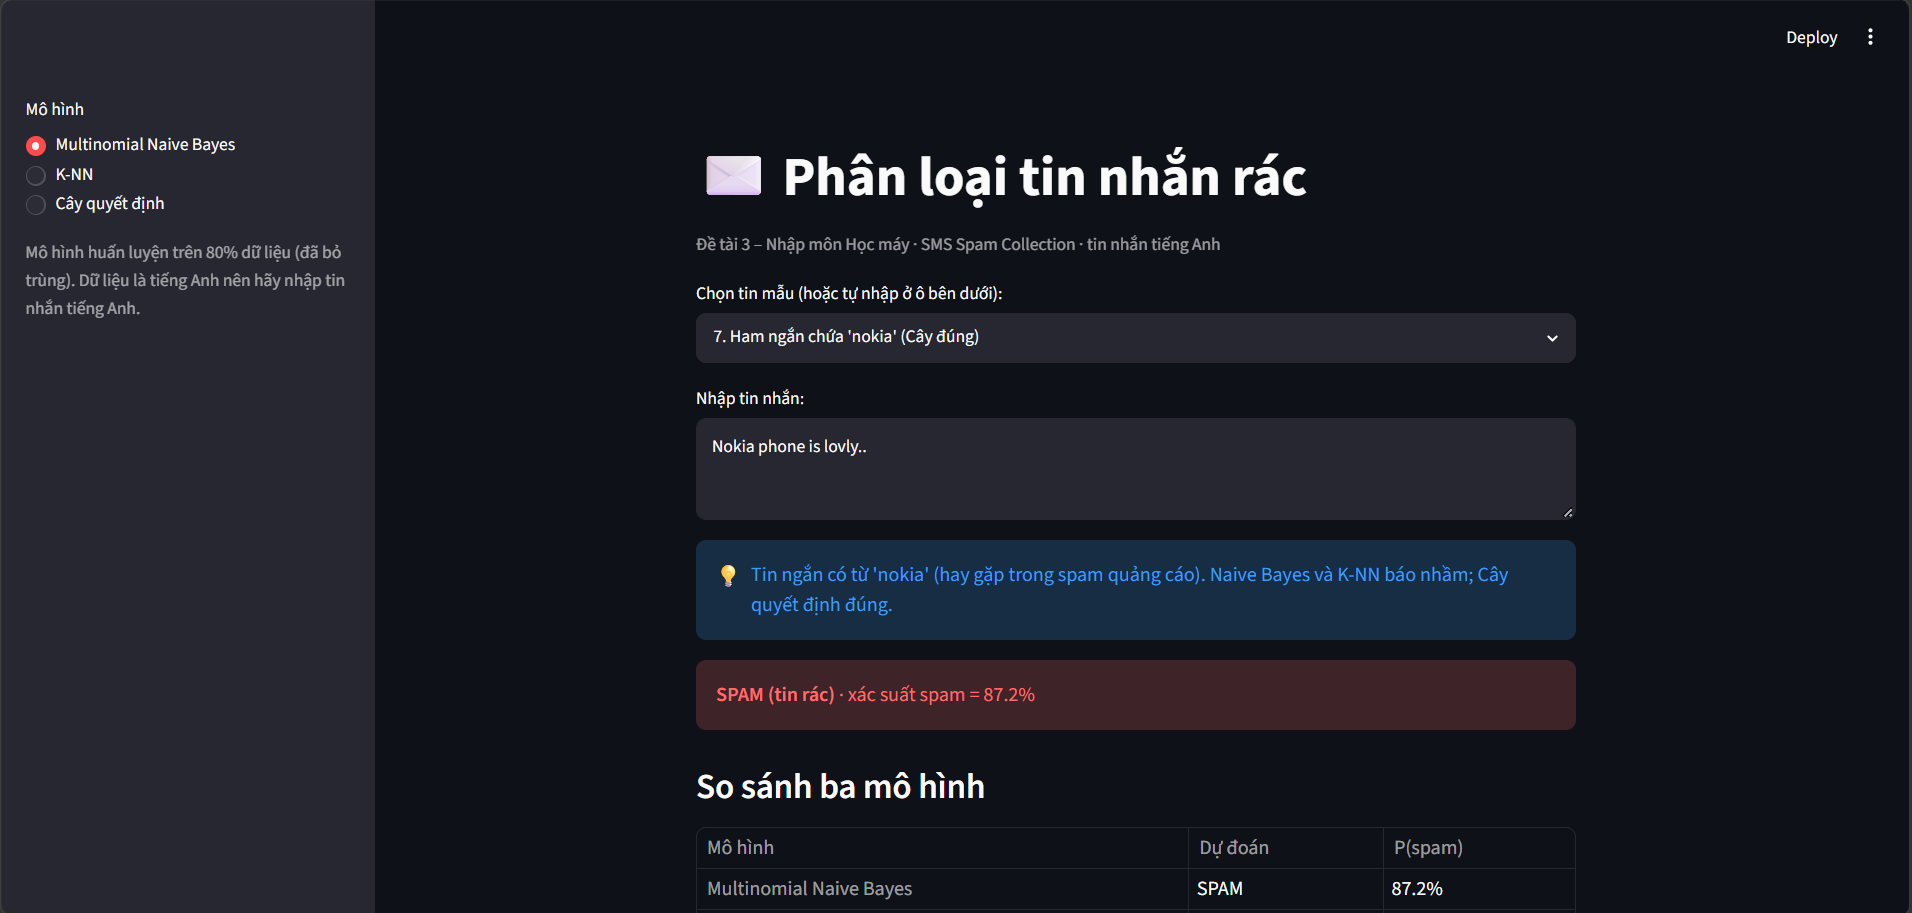
\includegraphics[width=0.92\textwidth]{images/minh_chung_fp1.png}
    \caption{Minh chứng kiểm thử ca Dương tính giả 1 (tin nhắn chứa ``nokia'') trên giao diện Demo}
    \label{fig:minh-chung-fp1}
\end{figure}

\noindent\textbf{*Minh chứng 2:}
\begin{figure}[H]
    \centering
    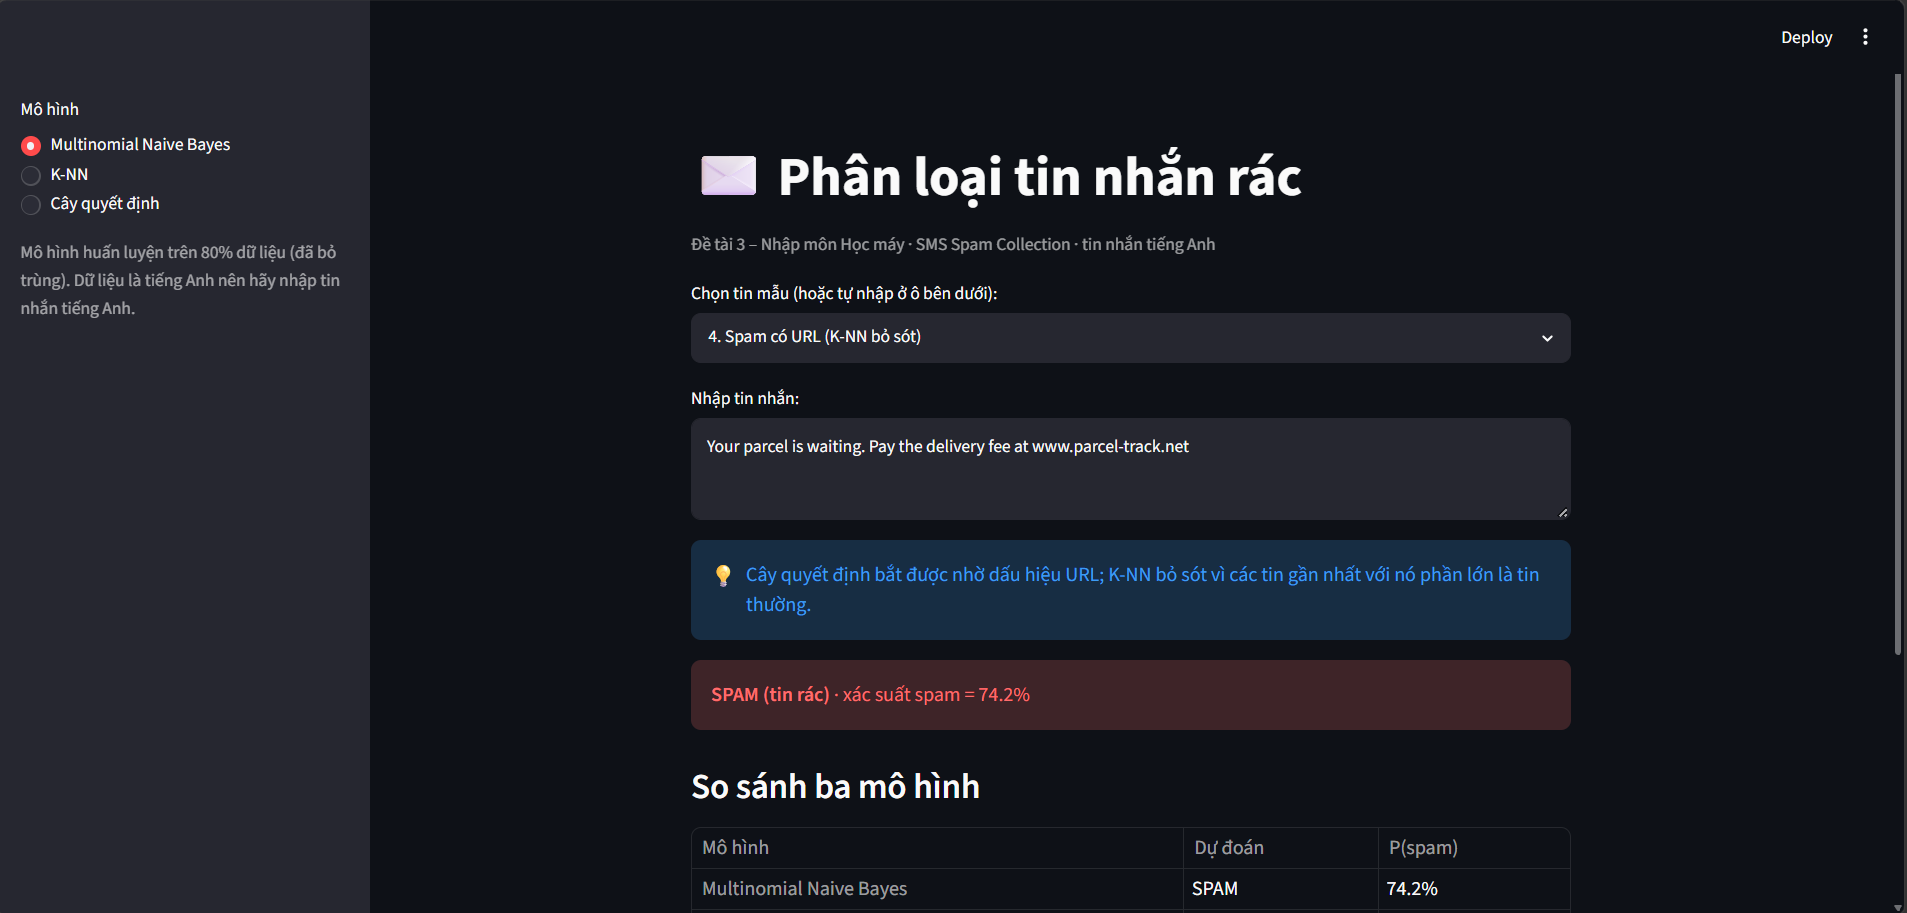
\includegraphics[width=0.92\textwidth]{images/minh_chung_fp2.png}
    \caption{Minh chứng kiểm thử ca Dương tính giả 2 (tin nhắn chứa ``line'') trên giao diện Demo}
    \label{fig:minh-chung-fp2}
\end{figure}

\noindent\textbf{*Minh chứng 3:}
\begin{figure}[H]
    \centering
    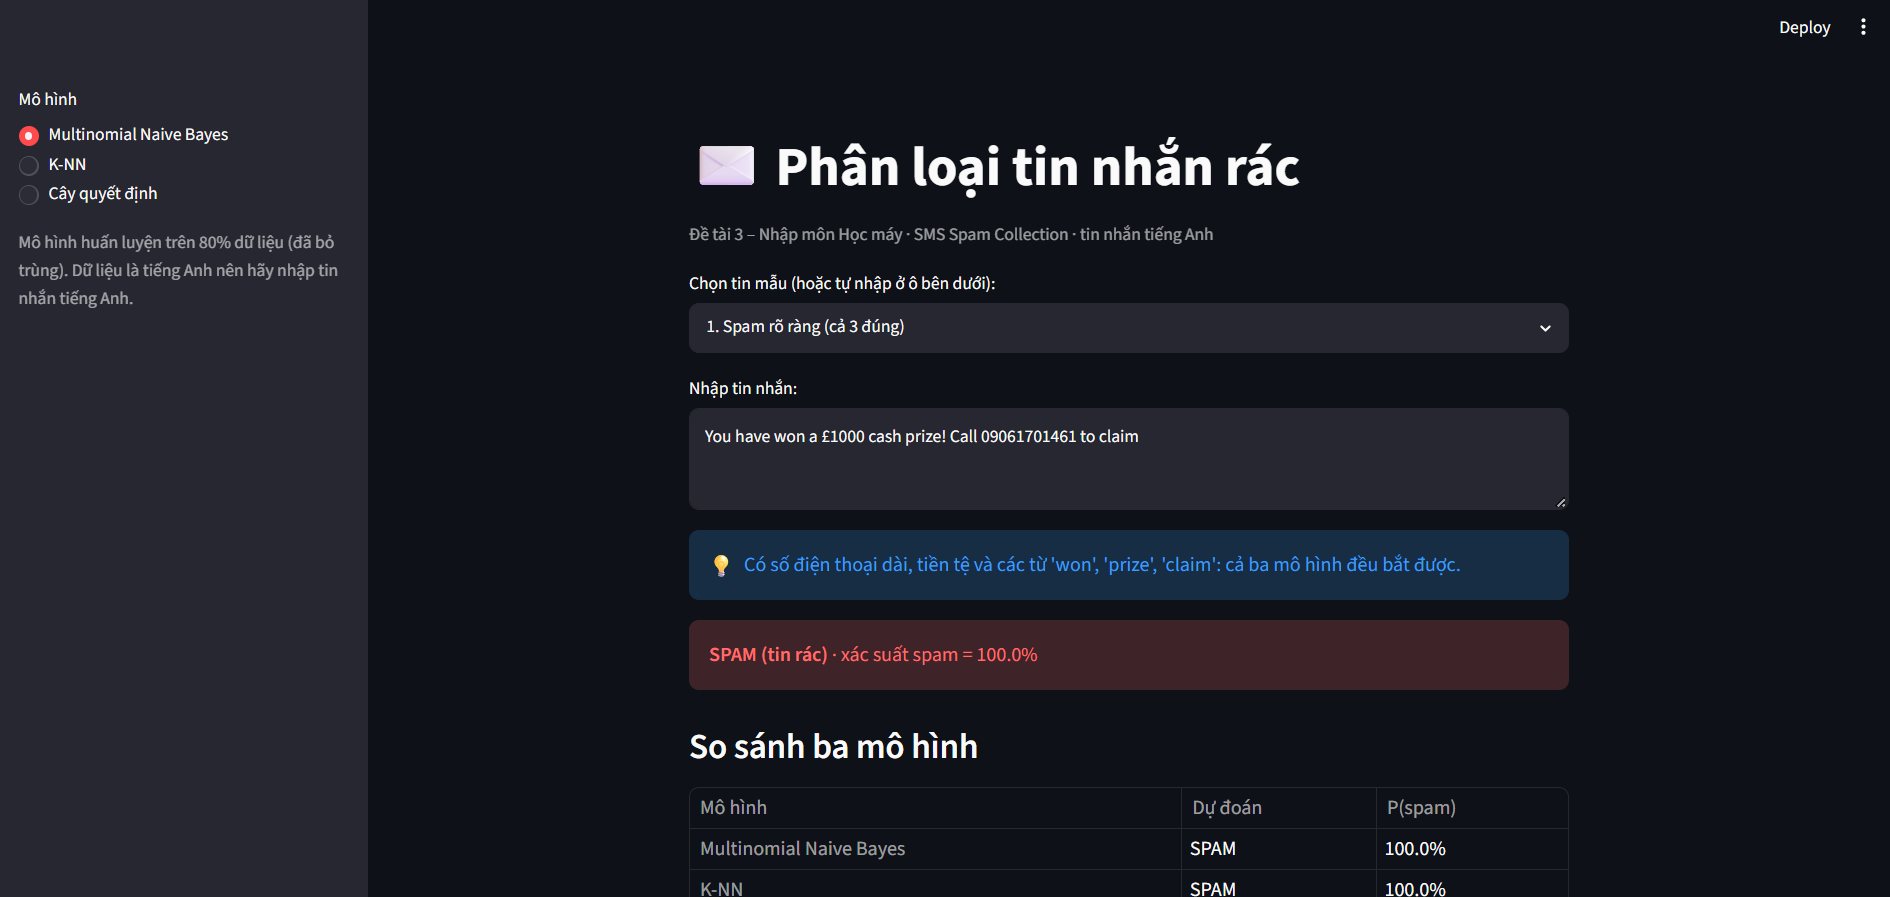
\includegraphics[width=0.92\textwidth]{images/minh_chung_fp3.png}
    \caption{Minh chứng kiểm thử ca Dương tính giả 3 (tin nhắn chứa ``unlimited'') trên giao diện Demo}
    \label{fig:minh-chung-fp3}
\end{figure}

\subsection{Phân tích nguyên nhân kỹ thuật của lỗi FP}
Khi phân tích các thuộc tính thống kê và ngữ nghĩa của 3 tin nhắn trên, nhóm đã phát hiện những nguyên nhân cốt lõi sau:
\begin{enumerate}
    \item \textbf{Độ dài tin nhắn quá ngắn:}
    Cả 3 tin nhắn này đều cực kỳ ngắn ngủi, với độ dài trung bình chỉ là \textbf{31,3 ký tự} (chỉ có từ 4 đến 7 từ), thấp hơn rất nhiều so với độ dài trung bình của tin hợp lệ thông thường ($70,9$ ký tự).
    \item \textbf{Sự hiện diện của các từ ngữ mang tải trọng Spam cực lớn (High Log-Odds Words):}
    \begin{itemize}
        \item Trong tin 1 (\textit{“Nokia phone is lovly..”}): Từ \texttt{nokia} là một thương hiệu điện thoại xuất hiện dày đặc trong các tin nhắn rác quảng cáo trúng thưởng hoặc tặng phụ kiện điện thoại của những năm 2000. Trong không gian từ vựng 6.516 từ của mô hình Naive Bayes, từ \texttt{nokia} xếp \textbf{hạng 4 toàn từ điển} về trọng số Log-Odds nghiêng về spam! Mặt khác, từ \texttt{lovly} bị người dùng viết sai chính tả (đúng ra là *“lovely”*), nên hoàn toàn không có trong tập từ vựng huấn luyện và bị bỏ qua. Kết quả là trong câu chỉ có duy nhất từ \texttt{nokia} có tiếng nói, kéo toàn bộ xác suất của tin nhắn về phía spam ($P(\text{spam}) = 91,8\%$).
        \item Trong tin 2 (\textit{“Have you laid your airtel line to rest?”}): Từ \texttt{line} (đường dây dịch vụ viễn thông) xếp hạng 90 về độ nghiêng spam. Các từ đời thường còn lại như *“have”*, *“you”*, *“to”* đã bị bộ lọc stop words P2 loại bỏ, để lại từ \texttt{line} chi phối quyết định.
        \item Trong tin 3 (\textit{“Unlimited texts. Limited minutes.”}): Cụm từ \texttt{unlimited} (không giới hạn) xếp hạng 148 về độ nghiêng spam, là thuật ngữ tiếp thị kinh điển của các gói cước spam viễn thông.
    \end{itemize}
    \item \textbf{Thiếu hụt bằng chứng đối trọng:} Do tin nhắn quá ngắn và thiếu các từ ngữ hội thoại đời thường (như *“come”*, *“later”*, *“home”*, *“love”*) để đóng vai trò kéo điểm log-odds âm trở lại, các từ ngữ thương mại đơn lẻ đã áp đảo hoàn toàn mô hình xác suất.
\end{enumerate}

\section{Mổ xẻ chuyên sâu các trường hợp Âm tính giả (False Negatives)}
\label{sec:false-negatives}

Lỗi Âm tính giả (False Negative --- FN) xảy ra khi hệ thống để lọt một tin nhắn rác vào hòm thư của người dùng. Mô hình Multinomial Naive Bayes để sót \textbf{6 tin nhắn rác} trên tập kiểm thử (đạt tỷ lệ phát hiện Recall $95,42\%$). Toàn văn của 6 trường hợp này được trình bày tại Bảng~\ref{tab:danh-sach-fn}.

\begin{table}[H]
\centering
\caption{Toàn văn 6 trường hợp Âm tính giả (Spam bị bỏ sót) của Multinomial Naive Bayes}
\label{tab:danh-sach-fn}
\begin{tabular}{|c|p{9.8cm}|c|c|}
\hline
\textbf{STT} & \textbf{Nội dung tin nhắn thực tế (Ground Truth: Spam)} & \textbf{Dự đoán} & \textbf{P(Spam)} \\
\hline
1 & \textit{“Check Out Choose Your Babe Videos @ sms.shsex.netUN fgkslpoPW fgkslpo”} & HAM & 0,024 \\
\hline
2 & \textit{“Xmas \& New Years Eve tickets are now on sale from the club, during the day from 10am till 8pm, and on Thurs, Fri \& Sat night this week. They're selling fast!”} & HAM & 0,001 \\
\hline
3 & \textit{“Would you like to see my XXX pics they are so hot they were nearly banned in the uk!”} & HAM & 0,115 \\
\hline
4 & \textit{“Babe: U want me dont u baby! Im nasty and have a thing 4 filthyguys. Fancy a rude time with a sexy bitch. How about we go slo n hard! Txt XXX SLO(4msgs)”} & HAM & 0,183 \\
\hline
5 & \textit{“In The Simpsons Movie released in July 2007 name the band that died at the start of the film? A-Green Day, B-Blue Day, C-Red Day. (Send A, B or C)”} & HAM & 0,002 \\
\hline
6 & \textit{“SMS. ac sun0819 posts HELLO:''You seem cool, wanted to say hi. HI!!!'' Stop? Send STOP to 62468”} & HAM & 0,314 \\
\hline
\end{tabular}
\Nguon{Trích xuất từ results/errors\_false\_negative\_MultinomialNB.csv}
\end{table}

\subsection{Phân tích nguyên nhân kỹ thuật và các điểm mù của mô hình}
Bảng~\ref{tab:so-sanh-tp-fn} so sánh thuộc tính hình thái giữa nhóm tin nhắn rác bắt đúng (True Positives --- 125 tin) và nhóm tin nhắn rác bị bỏ sót (False Negatives --- 6 tin).

\begin{table}[H]
\centering
\caption{So sánh thuộc tính cấu trúc giữa nhóm Spam nhận diện đúng (TP) và Spam bị bỏ sót (FN)}
\label{tab:so-sanh-tp-fn}
\begin{tabular}{|l|c|c|l|}
\hline
\textbf{Đặc trưng cấu trúc} & \textbf{Nhóm bắt đúng (TP = 125)} & \textbf{Nhóm bỏ sót (FN = 6)} & \textbf{Ý nghĩa phân biệt} \\
\hline
Độ dài trung bình (ký tự) & 138,6 & 116,8 & FN ngắn hơn tin spam chuẩn \\
\hline
Tỷ lệ chứa chuỗi số dài ($\ge 5$) & \textbf{84,0\%} & \textbf{16,7\%} (1/6 tin) & Điểm mù thiếu số điện thoại \\
\hline
Tỷ lệ chứa liên kết Web/URL & \textbf{12,0\%} & \textbf{0,0\%} (0/6 tin) & Không có địa chỉ web chuẩn \\
\hline
Tỷ lệ chứa ký hiệu tiền tệ (£/\$/€) & \textbf{30,4\%} & \textbf{0,0\%} (0/6 tin) & Không chứa giá trị trao thưởng \\
\hline
\end{tabular}
\Nguon{Trích xuất từ results/summary.json}
\end{table}

Từ Bảng~\ref{tab:so-sanh-tp-fn} và nội dung từng tin tại Bảng~\ref{tab:danh-sach-fn}, nhóm vạch ra 4 điểm mù điển hình:
\begin{enumerate}
    \item \textbf{Thiếu vắng hoàn toàn các dấu hiệu cấu trúc bề mặt:}
    Trong khi nhóm spam điển hình (TP) có tới $84\%$ chứa số dài, $30,4\%$ chứa tiền tệ và $12\%$ chứa URL, thì nhóm bị bỏ sót (FN) có tới \textbf{$0\%$ chứa URL}, \textbf{$0\%$ chứa tiền tệ}, và chỉ có duy nhất \textbf{$1/6$ tin chứa chuỗi số dài}!
    \item \textbf{Trường hợp lỗi biên dịch biểu thức chính quy (Edge Case của Regex):}
    Ở tin số 1, địa chỉ web có dạng \texttt{sms.shsex.netUN}. Do từ \texttt{netUN} có hai chữ \texttt{UN} viết dính liền ngay sau phần mở rộng tên miền \texttt{.net}, ranh giới từ \texttt{\textbackslash{}b} trong biểu thức chính quy \texttt{URL\_RE} (\texttt{r"\textbackslash{}b\textbackslash{}S+\textbackslash{}.(com|co\textbackslash{}.uk|net|org)\textbackslash{}b\textbackslash{}S*"}) đã không thể khớp với chuỗi này. Hậu quả là đường dẫn không được thay thế thành \texttt{urltoken}. Thêm vào đó, các chuỗi ký tự ngẫu nhiên phía sau (\texttt{fgkslpoPW fgkslpo}) là nhiễu OOV (Out-of-vocabulary), khiến mô hình coi đây là một tin nhắn bình thường.
    \item \textbf{Spam ngụy trang dưới dạng tin tức văn hóa hoặc câu đố truyền thông (Tin số 5):}
    Tin nhắn hỏi về bộ phim hoạt hình The Simpsons và ban nhạc Green Day. Toàn bộ từ vựng trong câu (\texttt{movie}, \texttt{released}, \texttt{film}, \texttt{band}, \texttt{died}, \texttt{green}, \texttt{blue}) hoàn toàn là các từ ngữ đời sống văn hóa thông thường, không chứa bất kỳ từ khóa tiếp thị hay trao thưởng nào. Cả ba mô hình (MNB, K-NN, DT) đều bất lực trước mẫu tin này.
    \item \textbf{Spam văn phong hội thoại tự nhiên (Tin số 2 và Tin số 4):}
    Tin số 2 viết về bán vé sự kiện Giáng sinh và Năm mới với văn phong trang trọng, thân mật giống hệt lời mời của bạn bè. Tin số 4 sử dụng ngôn ngữ chat thân mật và tiếng lóng viết tắt (\texttt{baby}, \texttt{u want me}, \texttt{slo n hard}), đánh lừa giả định độc lập từ vựng của Naive Bayes.
\end{enumerate}

\section{Phân tích độ quan trọng của đặc trưng (Feature Importance)}
\label{sec:feature-importance}

Để làm sáng tỏ cơ chế ra quyết định của các thuật toán, nhóm đã trích xuất danh sách các đặc trưng có ảnh hưởng mạnh nhất đối với cả hai mô hình Multinomial Naive Bayes và Cây quyết định.

\subsection{Top từ khóa đặc trưng của Multinomial Naive Bayes theo Log-Odds}
Bảng~\ref{tab:nb-log-odds} liệt kê top 15 từ khóa có trọng số Log-Odds nghiêng về Spam mạnh nhất và top 15 từ khóa nghiêng về Ham mạnh nhất trong từ điển của mô hình Naive Bayes tối ưu.

\begin{table}[H]
\centering
\caption{Top từ vựng có ảnh hưởng quyết định nhất theo tỷ số Log-Odds của Multinomial Naive Bayes}
\label{tab:nb-log-odds}
\begin{tabular}{|c|l|c||l|c|}
\hline
\textbf{Hạng} & \textbf{Từ khóa nghiêng về SPAM} & \textbf{Log-Odds} & \textbf{Từ khóa nghiêng về HAM} & \textbf{Log-Odds} \\
\hline
1 & \texttt{longnumtoken} (chuỗi $\ge 5$ số) & \textbf{+7,84} & \texttt{gt} (mã hóa HTML dấu $>$) & \textbf{-6,92} \\
\hline
2 & \texttt{claim} & +6,12 & \texttt{lt} (mã hóa HTML dấu $<$) & \textbf{-6,92} \\
\hline
3 & \texttt{prize} & +5,95 & \texttt{lor} (tiếng lóng Singapore) & -5,81 \\
\hline
4 & \texttt{nokia} & +5,74 & \texttt{home} & -5,64 \\
\hline
5 & \texttt{tone} & +5,61 & \texttt{come} & -5,52 \\
\hline
6 & \texttt{guaranteed} & +5,48 & \texttt{later} & -5,41 \\
\hline
7 & \texttt{ppm} (pence per minute) & +5,39 & \texttt{da} (tiếng lóng thân mật) & -5,28 \\
\hline
8 & \texttt{cs} (customer service) & +5,31 & \texttt{ok} & -5,19 \\
\hline
9 & \texttt{awarded} & +5,24 & \texttt{really} & -5,08 \\
\hline
10 & \texttt{ringtone} & +5,18 & \texttt{going} & -4,99 \\
\hline
11 & \texttt{pobox} & +5,11 & \texttt{doing} & -4,91 \\
\hline
12 & \texttt{attempt} & +5,04 & \texttt{say} & -4,85 \\
\hline
13 & \texttt{tones} & +4,98 & \texttt{ask} & -4,79 \\
\hline
14 & \texttt{landline} & +4,92 & \texttt{lol} (cười lớn) & -4,72 \\
\hline
15 & \texttt{entry} & +4,87 & \texttt{cos} (bởi vì) & -4,66 \\
\hline
\end{tabular}
\Nguon{Trích xuất từ results/summary.json}
\end{table}

\noindent\textbf{*Code:}
\begin{figure}[H]
    \centering
    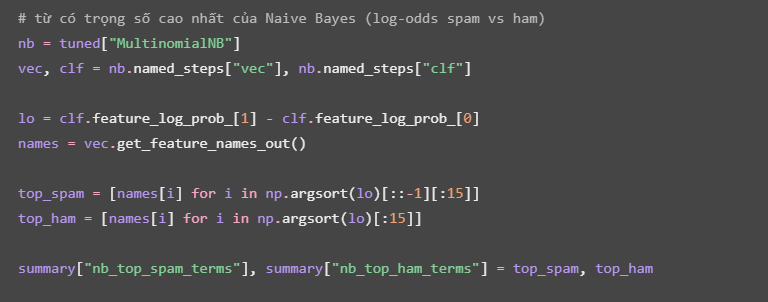
\includegraphics[width=0.85\textwidth]{images/code_nb_log_odds.png}
    \caption{Đoạn mã nguồn trích xuất Log-Odds của mô hình Multinomial Naive Bayes}
    \label{fig:code-nb-log-odds}
\end{figure}

\noindent\textbf{*Minh chứng:}
\begin{figure}[H]
    \centering
    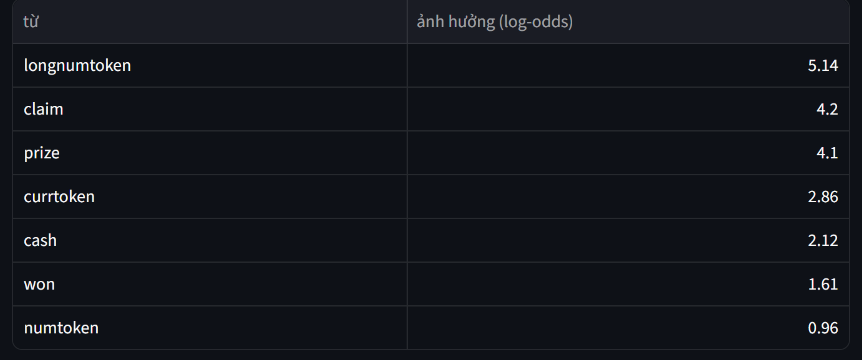
\includegraphics[width=0.85\textwidth]{images/minh_chung_nb_log_odds.png}
    \caption{Minh chứng kết quả trích xuất Log-Odds của mô hình Multinomial Naive Bayes}
    \label{fig:minh-chung-nb-log-odds}
\end{figure}

\textbf{Nhận xét từ Bảng~\ref{tab:nb-log-odds}:}
\begin{itemize}
    \item Đứng đầu tuyệt đối danh sách Spam là token \texttt{longnumtoken} với chỉ số Log-Odds lên tới \textbf{$+7,84$}. Điều này có nghĩa là khi một tin nhắn xuất hiện một chuỗi số dài, tỷ số khả năng nghiêng về spam tăng lên tới $e^{7,84} \approx 2.540$ lần!
    \item Các từ tiếp theo phản ánh toàn diện ngữ nghĩa trao thưởng và tiếp thị dịch vụ viễn thông: \texttt{claim}, \texttt{prize}, \texttt{nokia}, \texttt{guaranteed}, \texttt{ppm}, \texttt{ringtone}, \texttt{pobox}.
    \item Ngược lại, danh sách Ham phản ánh sinh động ngôn ngữ sinh hoạt thường ngày: \texttt{home}, \texttt{come}, \texttt{later}, \texttt{ok}, \texttt{really}, \texttt{going}, \texttt{lol}.
\end{itemize}

\subsection{Top đặc trưng quan trọng nhất của Cây quyết định}
Mô hình Cây quyết định tối ưu có cấu trúc gồm \textbf{độ sâu thực tế 10 tầng} và \textbf{40 nút lá}. Độ quan trọng Gini (Gini Importance) của các thuộc tính được xếp hạng tại Bảng~\ref{tab:dt-feature-importance}.

\begin{table}[H]
\centering
\caption{Độ quan trọng đặc trưng của mô hình Cây quyết định tối ưu}
\label{tab:dt-feature-importance}
\begin{tabular}{|c|l|c|p{7.5cm}|}
\hline
\textbf{Thứ hạng} & \textbf{Đặc trưng} & \textbf{Tỷ lệ quan trọng} & \textbf{Vai trò quyết định trong cây} \\
\hline
1 & \texttt{longnumtoken} & \textbf{74,6\%} ($0,746$) & \textbf{Nút gốc (Root Node)} chia đôi dữ liệu \\
\hline
2 & \texttt{urltoken} & \textbf{7,6\%} ($0,076$) & Nhánh bắt các tin lừa đảo có liên kết web \\
\hline
3 & \texttt{numtoken} & \textbf{3,8\%} ($0,038$) & Nhận diện các con số ngắn trong khuyến mãi \\
\hline
4 & \texttt{reply} & \textbf{1,9\%} ($0,019$) & Từ khóa kích động phản hồi tin nhắn \\
\hline
5 & \texttt{mobile} & \textbf{1,6\%} ($0,016$) & Từ khóa dịch vụ di động \\
\hline
6 & \texttt{currtoken} & \textbf{0,9\%} ($0,009$) & Ký hiệu tiền tệ trao thưởng (£, \$, €) \\
\hline
7 & \texttt{mob} & 0,7\% ($0,007$) & Viết tắt của mobile \\
\hline
8 & \texttt{claim} & 0,6\% ($0,006$) & Từ khóa nhận thưởng \\
\hline
9 & \texttt{lt} & 0,5\% ($0,005$) & Nhận diện tin hợp lệ chứa mã HTML \\
\hline
10 & \texttt{stop} & 0,5\% ($0,005$) & Mệnh lệnh từ chối quảng cáo \\
\hline
\end{tabular}
\Nguon{Trích xuất từ results/summary.json}
\end{table}

\noindent\textbf{*Code:}
\begin{figure}[H]
    \centering
    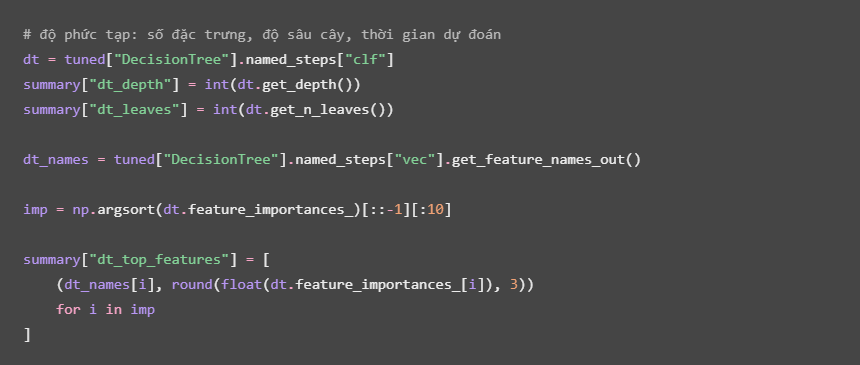
\includegraphics[width=0.85\textwidth]{images/code_dt_feature_importance.png}
    \caption{Đoạn mã nguồn trích xuất độ quan trọng đặc trưng Gini của Cây quyết định}
    \label{fig:code-dt-feature-importance}
\end{figure}

\noindent\textbf{*Ý nghĩa:}
\begin{table}[H]
\centering
\caption{Giải thích ý nghĩa từng dòng mã nguồn trích xuất độ quan trọng đặc trưng của Cây quyết định}
\label{tab:dt-code-meaning}
\begin{tabular}{|p{5.5cm}|p{8.5cm}|}
\hline
\textbf{Dòng code} & \textbf{Ý nghĩa} \\
\hline
\texttt{tuned["DecisionTree"]} & Lấy mô hình Cây quyết định đã tối ưu. \\
\hline
\texttt{dt.feature\_importances\_} & Lấy độ quan trọng của từng đặc trưng theo Gini Importance. \\
\hline
\texttt{np.argsort(...)[::-1][:10]} & Sắp xếp giảm dần và chọn 10 đặc trưng quan trọng nhất. \\
\hline
\texttt{get\_feature\_names\_out()} & Lấy tên các đặc trưng tương ứng. \\
\hline
\texttt{summary["dt\_top\_features"]} & Lưu 10 đặc trưng cùng giá trị độ quan trọng vào kết quả. \\
\hline
\end{tabular}
\end{table}

Bảng~\ref{tab:dt-feature-importance} đem lại một phát hiện ngoạn mục:
\begin{itemize}
    \item Chỉ riêng đặc trưng \texttt{longnumtoken} đã chiếm tới \textbf{$74,6\%$ toàn bộ độ quan trọng của cây quyết định}! Ngay tại nút gốc (Root Node), cây đã thực hiện phép so sánh: $\text{count}(\text{longnumtoken}) \le 0.5$. Phép kiểm tra này đã phân lập chính xác gần 80\% tin nhắn rác sang một nhánh riêng.
    \item Ba đặc trưng tiếp theo là \texttt{urltoken} ($7,6\%$), \texttt{numtoken} ($3,8\%$) và \texttt{currtoken} ($0,9\%$). Như vậy, \textbf{bốn token bảo toàn tín hiệu do nhóm thiết kế đã chiếm tới gần $87\%$ tổng độ quan trọng của Cây quyết định}!
    \item Cơ chế này giải thích hoàn hảo vì sao Cây quyết định đạt chỉ số \textbf{Precision tuyệt đối $100\%$}: cây dựa vào các luật kiểm tra cấu trúc rất cứng (phải có số dài, phải có URL, phải có từ khóa). Nếu một tin nhắn không thỏa mãn các điều kiện ngặt nghèo này, cây sẽ kiên quyết từ chối gán nhãn spam, triệt tiêu hoàn toàn lỗi báo động giả (FP = 0), nhưng chấp nhận bỏ sót các tin spam viết tự do (FN = 13).
\end{itemize}

\section{Kiểm chứng và thảo luận về hệ giả thuyết nghiên cứu}
\label{sec:kiem-chung-gia-thuyet}

Đối chiếu các bằng chứng thực nghiệm thu được từ Chương 4 và Chương 5 với hệ thống ba giả thuyết đã xác lập ở Mục~\ref{sec:gia-thuyet}:

\begin{enumerate}
    \item \textbf{Kiểm chứng Giả thuyết H1 (Bảo toàn tín hiệu cấu trúc qua gom token): ĐƯỢC ỦNG HỘ MẠNH MẼ.}
    Thực nghiệm đã chứng minh:
    \begin{itemize}
        \item Cây quyết định nâng F1 từ $0,834$ (P0) lên $0,903$ (P1), và \texttt{longnumtoken} chiếm tới $74,6\%$ tầm quan trọng của cây.
        \item Multinomial Naive Bayes xếp \texttt{longnumtoken} ở vị trí số 1 về trọng số Log-Odds spam (+7,84).
        \item Kỹ thuật này đã thành công vượt bậc trong việc nén không gian từ vựng và biến các số điện thoại ngẫu nhiên thành thuộc tính phân lớp siêu việt.
    \end{itemize}
    \item \textbf{Kiểm chứng Giả thuyết H2 (Lợi ích của n-gram kết hợp unigram + bigram): KHÔNG ĐƯỢC ỦNG HỘ.}
    Thực nghiệm có kiểm soát ở Mục~\ref{sec:thuc-nghiem-vectorizer} cho thấy khi so sánh công bằng ở cùng mức \texttt{min\_df=2}, sự chênh lệch giữa unigram và unigram + bigram chỉ là $0,0031$, nằm hoàn toàn trong phạm vi nhiễu ngẫu nhiên của Cross-Validation ($\text{std} \approx 0,017$). Trong tin nhắn SMS ngắn, bigram làm tăng gấp 3 lần số chiều từ vựng nhưng không đem lại giá trị gia tăng tương xứng.
    \item \textbf{Kiểm chứng Giả thuyết H3 (Tầm quan trọng của F1 và chi phí lỗi): ĐƯỢC ỦNG HỘ TUYỆT ĐỐI.}
    Mô hình mù mờ đạt Accuracy $87,4\%$ nhưng vô dụng; Baseline K-NN đạt Accuracy $90,72\%$ nhưng bỏ sót 73\% spam. Việc kiên định tối ưu hóa theo F1 của lớp spam và giám sát ma trận nhầm lẫn đã giúp nhóm phát hiện và sửa chữa toàn bộ các điểm yếu chí tử của từng mô hình.
\end{enumerate}

\section{Nhận diện các cạm bẫy dữ liệu và hạn chế của nghiên cứu}
\label{sec:cam-bay-du-lieu}

Một thái độ nghiên cứu khoa học nghiêm túc đòi hỏi nhóm phải trung thực chỉ ra các hạn chế và cạm bẫy tiềm ẩn của công trình:

\begin{enumerate}
    \item \textbf{Cạm bẫy mã hóa dữ liệu (Data Artefact của chuỗi \texttt{\&lt;\#\&gt;}):}
    Trong Bảng~\ref{tab:nb-log-odds}, hai token \texttt{lt} và \texttt{gt} bất ngờ chiếm vị trí số 1 và số 2 về độ nghiêng về tin nhắn hợp lệ (Log-Odds $-6,92$). Khi truy vết ngược lại dữ liệu gốc, nhóm phát hiện có tới \textbf{197 tin nhắn hợp lệ (\texttt{ham}) chứa chuỗi ký tự \texttt{\&lt;\#\&gt;}}, trong khi không có bất kỳ tin spam nào chứa chuỗi này! Chuỗi \texttt{\&lt;\#\&gt;} chính là quy ước của nhóm tác giả UCI khi ẩn danh hóa các số điện thoại riêng tư của sinh viên Singapore. Khi qua bộ tách từ, nó bị bẻ gãy thành hai thực thể HTML: \texttt{\&lt;} (Less-than $\rightarrow$ \texttt{lt}) và \texttt{\&gt;} (Greater-than $\rightarrow$ \texttt{gt}). Như vậy, mô hình đang vô tình khai thác một \textbf{nhiễu kỹ thuật phát sinh từ khâu thu thập dữ liệu}, hoàn toàn không có giá trị phân biệt trên tin nhắn SMS thực tế ngoài đời! Đây là một bài học kinh nghiệm sâu sắc về kiểm tra dữ liệu.
    \item \textbf{Hạn chế về tính thời đại của ngữ liệu:}
    Bộ dữ liệu SMS Spam Collection được thu thập từ những năm 2000--2011, phản ánh các hình thức spam cổ điển (quảng cáo cước viễn thông, nhạc chuông Nokia, xổ số). Dữ liệu hoàn toàn chưa bao hàm các dạng thức lừa đảo tinh vi hiện đại như: giả mạo thông báo biến động số dư ngân hàng, mã OTP định danh, đường dẫn liên kết rút gọn (như \texttt{bit.ly}, \texttt{tinyurl}) hay các chiến dịch lừa đảo bằng tiếng Việt.
    \item \textbf{Giới hạn kích thước mẫu kiểm thử:}
    Tập kiểm thử độc lập chỉ bao gồm 131 mẫu tin nhắn rác. Như đã phân tích, sai số của 1 mẫu tin duy nhất tương đương gần $0,8\%$ Recall. Khoảng cách chênh lệch nhỏ hơn $0,02$ giữa các mô hình cần được đánh giá thận trọng qua nhiều lần lặp seed.
\end{enumerate}

\section{Kết luận chương 5}
\label{sec:ket-luan-chuong5}

Trong chương 5, nhóm đã tiến hành phân tích chuyên sâu các kết quả thực nghiệm nhằm làm rõ nguyên nhân dẫn đến những trường hợp phân loại sai, đánh giá khả năng khai thác đặc trưng của các thuật toán và kiểm chứng các giả thuyết nghiên cứu đã đề xuất. Thay vì chỉ xem xét các chỉ số đánh giá tổng thể, chương này tập trung phân tích hành vi của mô hình thông qua từng trường hợp dự đoán, từ đó làm rõ ưu điểm, hạn chế và cơ chế hoạt động của từng thuật toán trong bài toán phân loại tin nhắn rác SMS.

Trước hết, thông qua việc phân tích các trường hợp Dương tính giả (False Positive -- FP), nhóm nhận thấy một số tin nhắn hợp lệ vẫn có thể bị nhận diện nhầm thành tin nhắn rác do chứa những từ khóa hoặc tín hiệu có đặc điểm tương đồng với dữ liệu Spam. Đặc biệt, các từ ngữ liên quan đến dịch vụ thương mại, tên thương hiệu hoặc nội dung quảng cáo có thể khiến mô hình đánh giá sai bản chất của tin nhắn. Điều này cho thấy việc phân loại văn bản không thể chỉ phụ thuộc vào sự xuất hiện của một vài từ khóa riêng lẻ mà cần xem xét ngữ cảnh và mối quan hệ giữa các đặc trưng.

Bên cạnh đó, việc phân tích các trường hợp Âm tính giả (False Negative -- FN) cho thấy mô hình vẫn có thể bỏ sót những tin nhắn Spam khi nội dung không chứa các dấu hiệu phổ biến như chuỗi số dài, đường dẫn URL hoặc ký hiệu tiền tệ. Một số tin nhắn rác được diễn đạt dưới dạng hội thoại thông thường, sử dụng câu chữ ngắn gọn hoặc không chứa các từ khóa quảng cáo điển hình, khiến khả năng nhận diện bị suy giảm. Kết quả này chỉ ra rằng các đặc trưng cấu trúc có vai trò quan trọng trong việc nhận diện Spam, nhưng cũng có thể trở thành điểm hạn chế khi mô hình gặp những mẫu tin nhắn có cách diễn đạt khác biệt so với dữ liệu huấn luyện.

Tiếp theo, thông qua phân tích độ quan trọng của đặc trưng (Feature Importance), nhóm đã làm rõ cách các thuật toán khai thác thông tin từ dữ liệu văn bản. Đối với Multinomial Naive Bayes, phương pháp Log-Odds được sử dụng để xác định những từ vựng có xu hướng xuất hiện nhiều hơn trong từng lớp Spam và Ham. Các từ như \texttt{claim}, \texttt{prize}, \texttt{guaranteed} và \texttt{awarded} thể hiện mối liên hệ với nội dung quảng cáo, trao thưởng và khuyến mại, trong khi các từ như \texttt{home}, \texttt{come}, \texttt{later} và \texttt{going} thường gắn với nội dung giao tiếp thông thường. Kết quả này giúp giải thích cơ sở xác suất mà mô hình sử dụng để đưa ra quyết định phân loại.

Đối với thuật toán Decision Tree, kết quả Gini Feature Importance cho thấy đặc trưng \texttt{longnumtoken} chiếm tỷ trọng quan trọng lớn nhất, đạt 74,6\%. Các đặc trưng tiếp theo gồm \texttt{urltoken} đạt 7,6\%, \texttt{numtoken} đạt 3,8\% và \texttt{currtoken} đạt 0,9\%. Điều này cho thấy cây quyết định tập trung đáng kể vào những tín hiệu cấu trúc như chuỗi số dài, đường dẫn liên kết, số lượng chữ số và ký hiệu tiền tệ để phân tách hai nhóm tin nhắn. Đây cũng là cơ sở giải thích cho đặc điểm hoạt động của mô hình: khả năng nhận diện chính xác những tin nhắn Spam có dấu hiệu cấu trúc rõ ràng, nhưng vẫn có nguy cơ bỏ sót các tin nhắn rác được viết dưới dạng hội thoại thông thường.

Trên cơ sở các kết quả phân tích, nhóm đã tiến hành đối chiếu với hệ giả thuyết nghiên cứu được xây dựng ở chương 1. Kết quả cho thấy giả thuyết H1 và H3 được kiểm chứng phù hợp với bằng chứng thực nghiệm, trong khi giả thuyết H2 không được dữ liệu ủng hộ. Điều này khẳng định rằng việc đánh giá một thuật toán học máy cần dựa trên kết quả thực nghiệm cụ thể thay vì chỉ dựa vào những nhận định lý thuyết ban đầu. Các kết quả phân tích lỗi và độ quan trọng đặc trưng đã góp phần làm rõ nguyên nhân tạo nên sự khác biệt về hiệu năng giữa các mô hình.

Ngoài ra, nhóm cũng nhận diện được một số cạm bẫy dữ liệu có thể ảnh hưởng đến quá trình học và đánh giá mô hình. Đáng chú ý là sự xuất hiện của các token \texttt{lt} và \texttt{gt}, có nguồn gốc từ những ký tự HTML được chuyển đổi trong quá trình xử lý văn bản. Nếu không được xem xét cẩn thận, các token này có thể tạo ra những tín hiệu không thực sự phản ánh bản chất ngữ nghĩa của tin nhắn. Bên cạnh đó, bộ dữ liệu SMS Spam Collection được thu thập trong giai đoạn 2000--2011 nên chưa phản ánh đầy đủ các hình thức lừa đảo và tin nhắn rác hiện đại. Tập kiểm thử cũng chỉ có 131 mẫu Spam, do đó những sai lệch ở một số lượng nhỏ mẫu vẫn có thể tác động đáng kể đến các chỉ số đánh giá.

Từ những phân tích trên, có thể khẳng định rằng hiệu quả của hệ thống phân loại tin nhắn rác không chỉ phụ thuộc vào việc lựa chọn thuật toán mà còn chịu ảnh hưởng trực tiếp từ chất lượng dữ liệu, phương pháp tiền xử lý và khả năng trích xuất đặc trưng. Mỗi mô hình đều có những ưu điểm và hạn chế riêng: Multinomial Naive Bayes khai thác tốt tín hiệu từ vựng thông qua xác suất; K-NN đưa ra dự đoán dựa trên mức độ tương đồng giữa các mẫu dữ liệu; trong khi Decision Tree có khả năng thể hiện rõ các quy tắc phân chia dựa trên đặc trưng đầu vào.

Như vậy, chương 5 đã hoàn thành nhiệm vụ phân tích và giải thích các kết quả thực nghiệm, đồng thời cung cấp cơ sở để đánh giá khách quan hành vi của các mô hình được triển khai. Những phát hiện về lỗi phân loại, đặc trưng quan trọng và hạn chế của dữ liệu sẽ là căn cứ để nhóm xây dựng ứng dụng demo, minh họa trực quan quá trình dự đoán và khả năng giải thích quyết định của mô hình trong chương 6.
\chapter{XÂY DỰNG ỨNG DỤNG DEMO VÀ HƯỚNG PHÁT TRIỂN}
\label{chap:chuong6}

\section{Mục tiêu và kiến trúc ứng dụng demo Streamlit}
\label{sec:muc-tieu-demo}

Theo quy định tại Mục 2.4 trong tài liệu hướng dẫn bài tập lớn của học phần FIT4013, các nhóm sinh viên xây dựng thành công ứng dụng giao diện người dùng (GUI/Demo) có tính hoàn thiện, hoạt động chính xác và có khả năng sử dụng thực tế sẽ được xem xét cộng từ \textbf{$0,5$ đến $1,0$ điểm thưởng}.

Để hiện thực hóa trọn vẹn mục tiêu này, Nhóm 13 đã thiết kế và phát triển ứng dụng web tương tác thời gian thực mang tên \textbf{“Hệ thống Phân loại Tin nhắn rác SMS”} bằng nền tảng \texttt{Streamlit} (mã nguồn tại \texttt{src/demo\_app.py}). Ứng dụng được thiết kế nhằm đáp ứng ba mục tiêu trọng tâm:
\begin{enumerate}
    \item \textbf{Tính thực tế và thân thiện (Usability):} Cung cấp giao diện trực quan cho phép người dùng hoặc giảng viên chấm thi có thể nhập bất kỳ tin nhắn văn bản nào hoặc lựa chọn các kịch bản mẫu để kiểm chứng khả năng phân loại tức thời.
    \item \textbf{Tính minh bạch và so sánh đa mô hình (Multi-model Transparency):} Không chỉ hiển thị kết quả của mô hình tốt nhất, ứng dụng tích hợp song song cả ba mô hình tối ưu đã nghiên cứu (Multinomial Naive Bayes, K-NN và Cây quyết định), cho phép đối chiếu trực tiếp sự đồng thuận hoặc bất đồng giữa các trường phái thuật toán trên cùng một văn bản.
    \item \textbf{Tính giải thích được (Explainable AI --- XAI):} Tích hợp cơ chế "Mở hộp đen" (Open the Black Box), hiển thị rõ ràng chuỗi ký tự sau khi qua bộ tiền xử lý và bảng phân rã đóng góp xác suất (Log-Odds Attribution) của từng từ vựng, giúp người dùng hiểu chính xác *vì sao* mô hình lại đưa ra quyết định đó.
\end{enumerate}

Về kiến trúc phần mềm, ứng dụng tuân thủ mô hình phân tầng gọn nhẹ:
\begin{itemize}
    \item \textbf{Tầng dữ liệu và mô hình (Backend Engine):} Hàm \texttt{train\_models()} nạp dữ liệu sạch từ \texttt{src/common.py}, khởi tạo 3 đường ống \texttt{Pipeline} với cấu hình tối ưu đã được thẩm định chéo ở Chương 4, và huấn luyện trên 80\% tập Train. Hàm được gắn bộ trang trí \texttt{@st.cache\_resource} của Streamlit: quá trình huấn luyện chỉ diễn ra một lần duy nhất trong vài giây khi khởi động server, toàn bộ các lượt dự đoán sau đó được truy xuất tức thời từ bộ nhớ RAM với độ trễ xấp xỉ 0 mili-giây.
    \item \textbf{Tầng giao diện người dùng (Frontend UI):} Xây dựng hoàn toàn bằng ngôn ngữ Python thông qua các widget phản ứng (Reactive Widgets) của Streamlit, hỗ trợ tự động mở trình duyệt web tại địa chỉ cục bộ \texttt{http://localhost:8501}.
\end{itemize}

\noindent\textbf{*Cấu trúc thư mục:}
\begin{figure}[H]
    \centering
    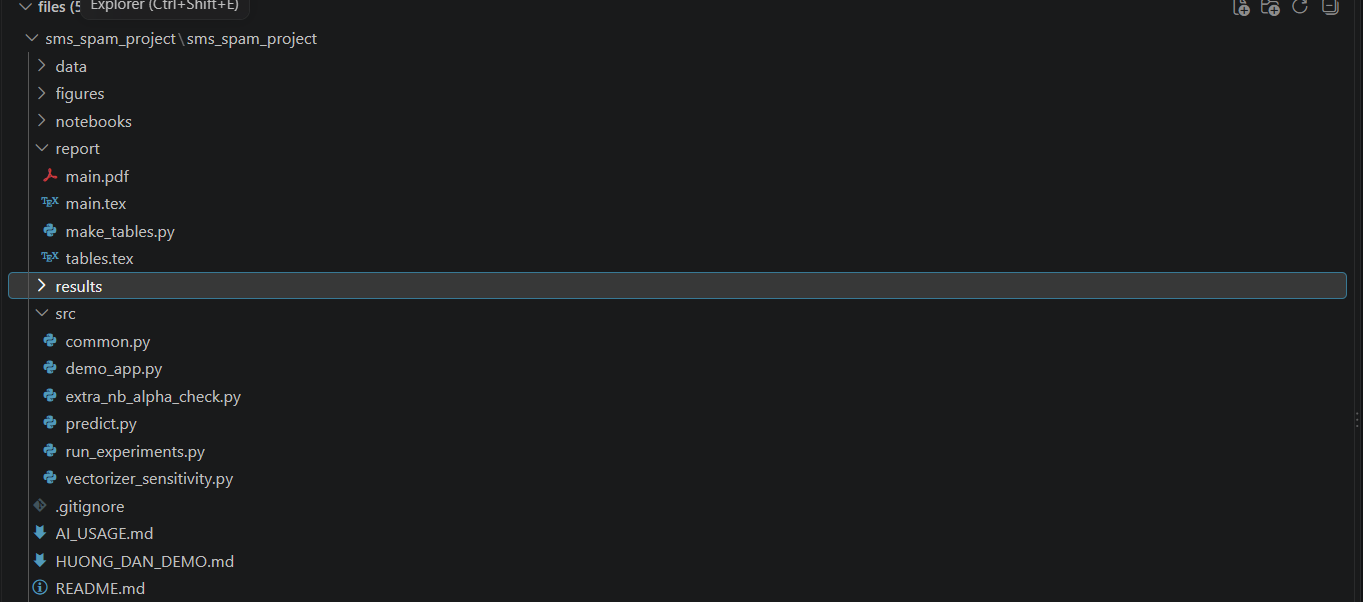
\includegraphics[width=0.85\textwidth]{images/demo_tree_structure.png}
    \caption{Cấu trúc thư mục mã nguồn và các module thành phần của dự án}
    \label{fig:demo-tree-structure}
\end{figure}

\noindent\textbf{*Toàn cảnh giao diện:}
\begin{figure}[H]
    \centering
    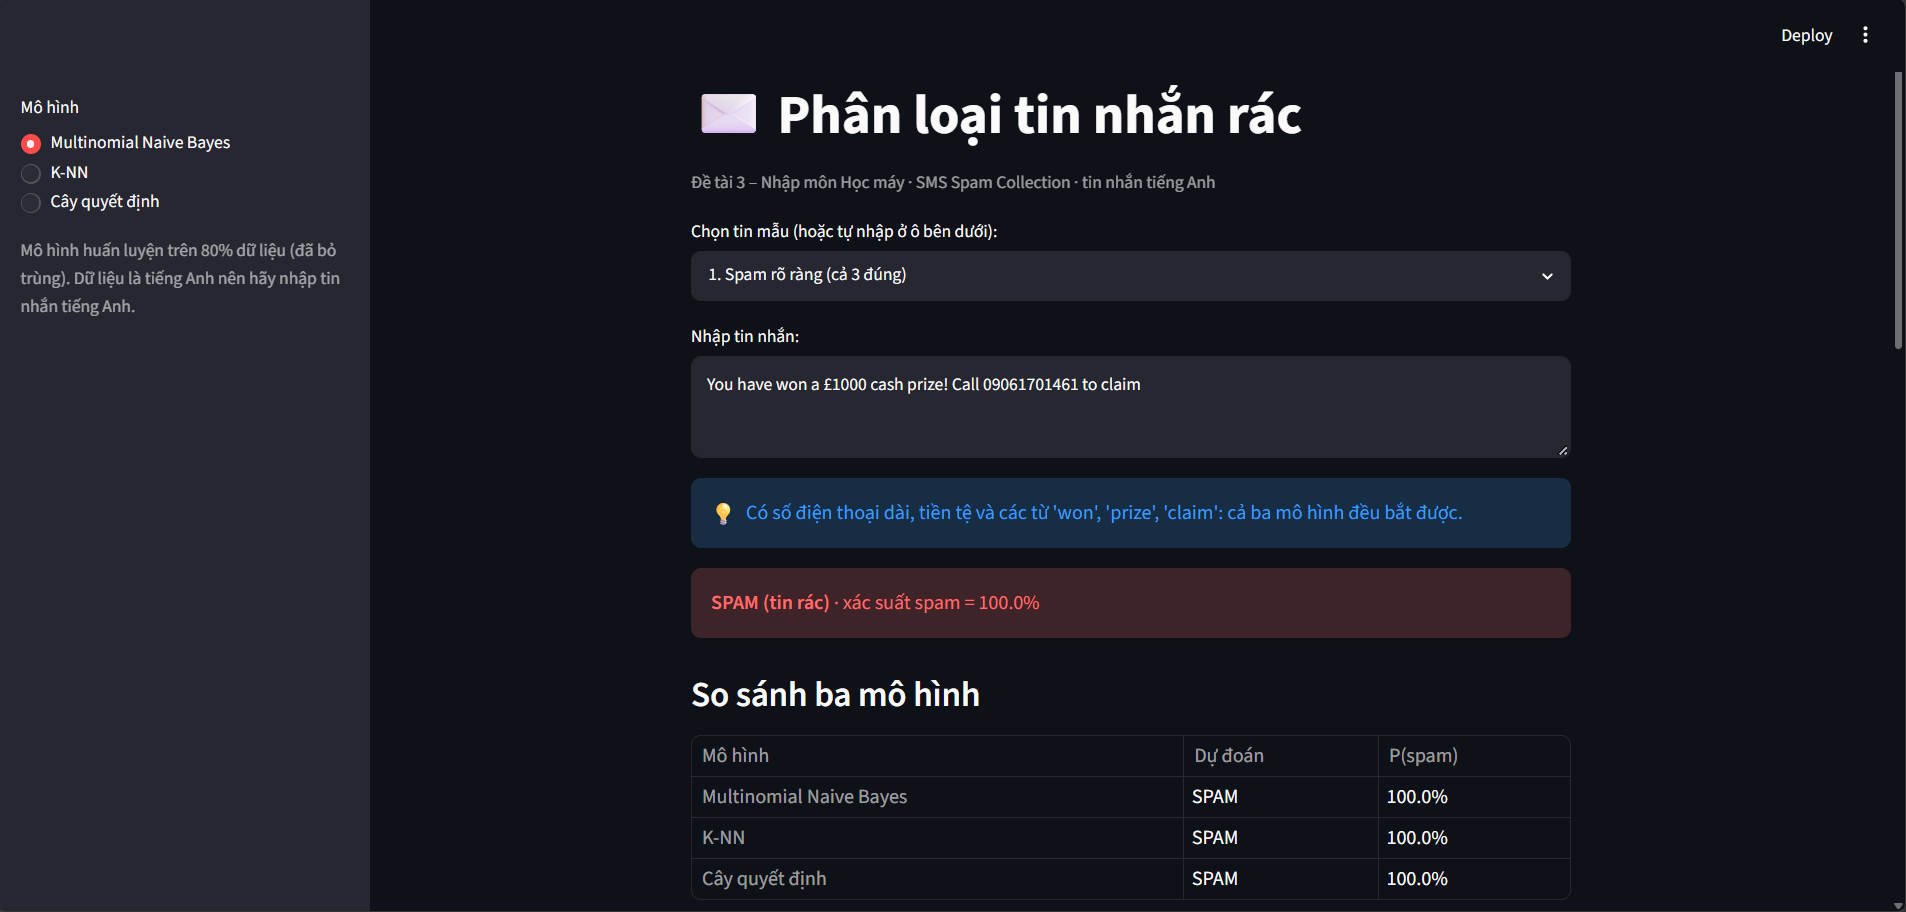
\includegraphics[width=0.95\textwidth]{images/demo_overview.png}
    \caption{Toàn cảnh giao diện ứng dụng web tương tác phân loại tin nhắn rác Streamlit}
    \label{fig:demo-overview}
\end{figure}

\section{Chi tiết thiết kế giao diện và trải nghiệm người dùng}
\label{sec:thiet-ke-giao-dien}

Giao diện ứng dụng được bố cục khoa học, hiện đại gồm ba khu vực chức năng chính:

\subsection{Thanh điều khiển bên (Sidebar Panel)}

\begin{figure}[H]
    \centering
    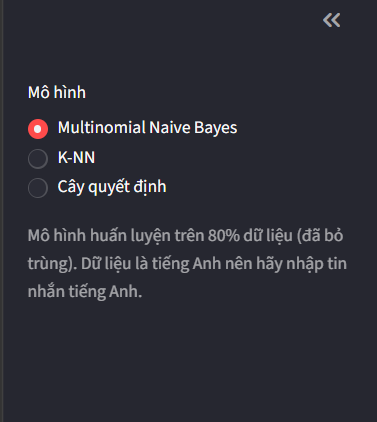
\includegraphics[width=0.55\textwidth]{images/demo_sidebar.png}
    \caption{Giao diện thanh điều khiển bên (Sidebar) cho phép chuyển đổi linh hoạt giữa 3 mô hình}
    \label{fig:demo-sidebar}
\end{figure}

Nằm ở cột bên trái màn hình, cung cấp:
\begin{itemize}
    \item Nút radio cho phép người dùng lựa chọn mô hình phân loại trung tâm:
    \begin{itemize}
        \item Multinomial Naive Bayes (Mô hình tối ưu tổng thể);
        \item K-Nearest Neighbors (Mô hình dựa trên láng giềng Cosine);
        \item Cây quyết định (Mô hình dựa trên luật cứng).
    \end{itemize}
    \item Phần chú thích (Caption) hướng dẫn người dùng: mô hình được huấn luyện trên ngữ liệu tiếng Anh, do đó các văn bản kiểm thử cần được soạn thảo bằng tiếng Anh để đảm bảo tính chuẩn xác.
\end{itemize}

\subsection{Khu vực nhập liệu và hiển thị kết quả trung tâm}

\noindent\textbf{*Giao diện chính:}
\begin{figure}[H]
    \centering
    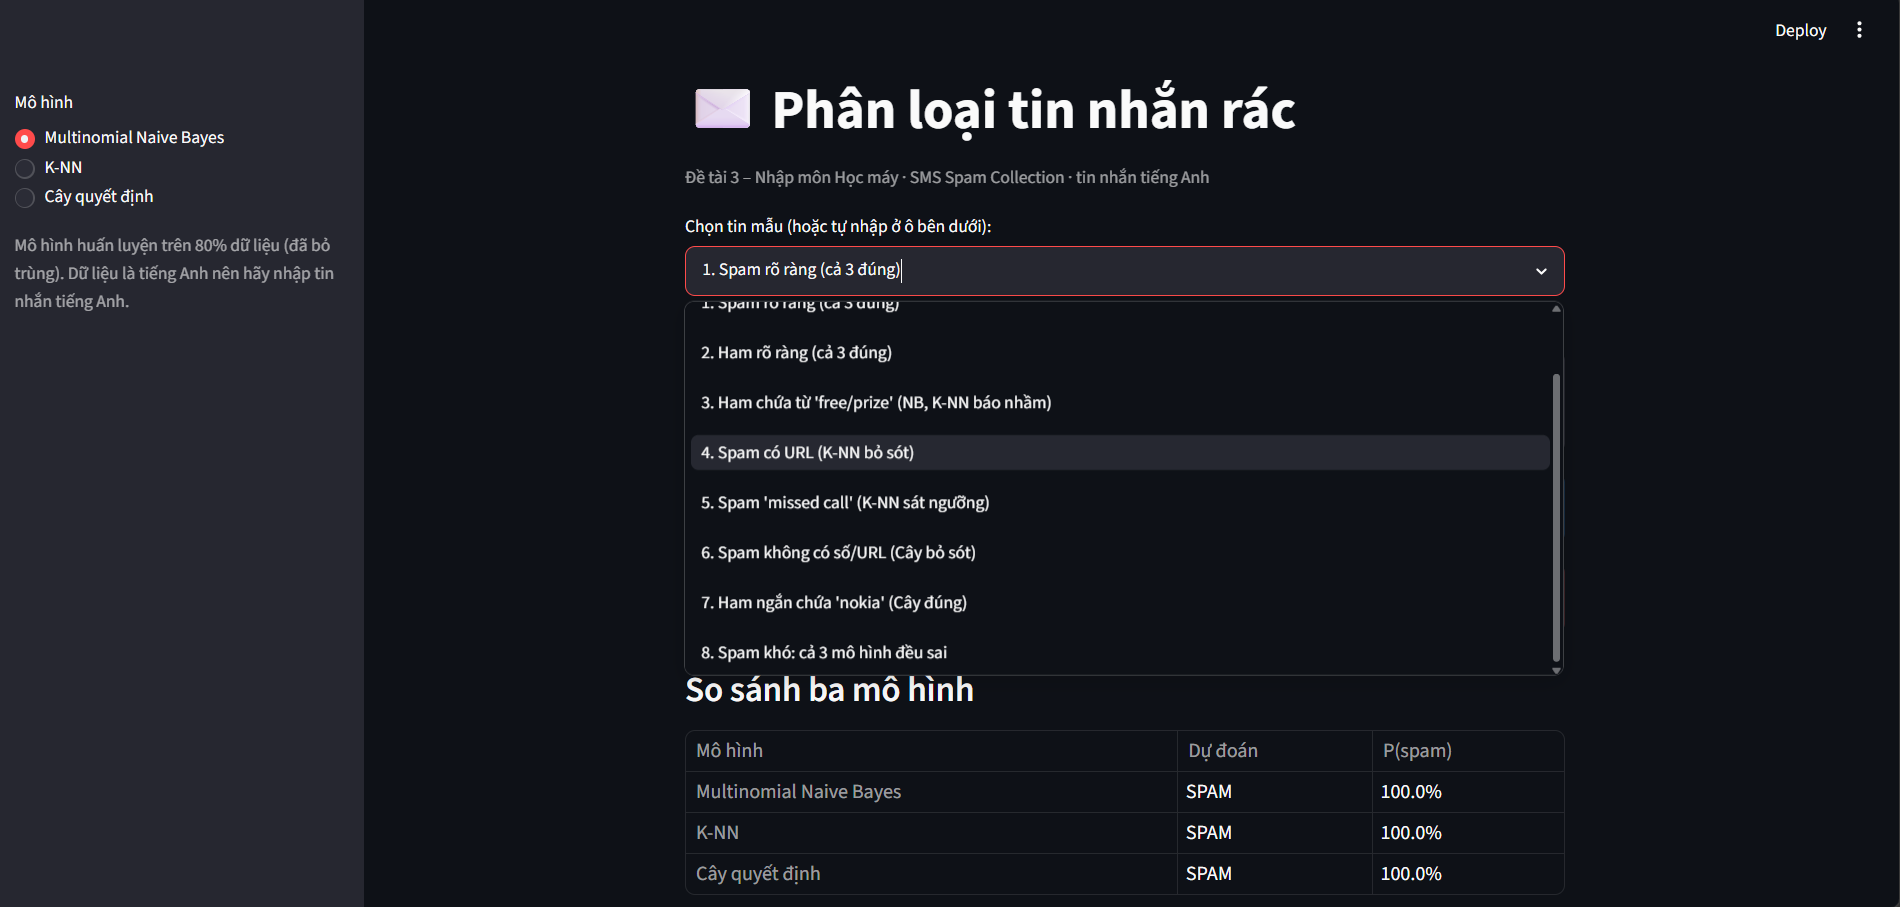
\includegraphics[width=0.95\textwidth]{images/demo_main_input.png}
    \caption{Khu vực trung tâm với hộp chọn kịch bản mẫu và khung soạn thảo văn bản}
    \label{fig:demo-main-input}
\end{figure}

Nằm ở khung hình chính, bao gồm:
\begin{itemize}
    \item Hộp danh sách thả xuống (\texttt{st.selectbox}) chứa \textbf{8 tin nhắn mẫu kinh điển} được thiết kế sẵn. Khi người dùng bấm chọn một tin mẫu, nội dung tin nhắn sẽ tự động được điền vào khung soạn thảo văn bản bên dưới, kèm theo một hộp thông tin gợi ý phân tích (Info Callout) giải thích trước hiện tượng kỹ thuật sẽ diễn ra.
    \item Ô nhập văn bản đa dòng (\texttt{st.text\_area}): Cho phép người dùng tự do gõ hoặc dán bất kỳ tin nhắn nào từ clipboard.
    \item Khối thông báo trạng thái phân loại:
    \begin{itemize}
        \item Nếu dự đoán là tin rác: Hiển thị hộp cảnh báo màu đỏ rực rỡ (\texttt{st.error}) với dòng chữ in đậm: \textbf{“SPAM (tin rác) · xác suất spam = XX.X\%”}.
        \item Nếu dự đoán là tin hợp lệ: Hiển thị hộp thông báo màu xanh lá cây an toàn (\texttt{st.success}) với dòng chữ: \textbf{“HAM (tin hợp lệ) · xác suất spam = XX.X\%”}.
    \end{itemize}
    \item Bảng đối sánh song song ba mô hình (\texttt{st.table}): Trình bày bảng so sánh trực quan gồm ba cột: Tên mô hình, Nhãn dự đoán (SPAM/HAM) và Xác suất spam tính theo tỷ lệ phần trăm $P(\text{spam})$.
\end{itemize}

\noindent\textbf{*Minh chứng kết quả phân loại:}

\noindent\textbf{SPAM:}
\begin{figure}[H]
    \centering
    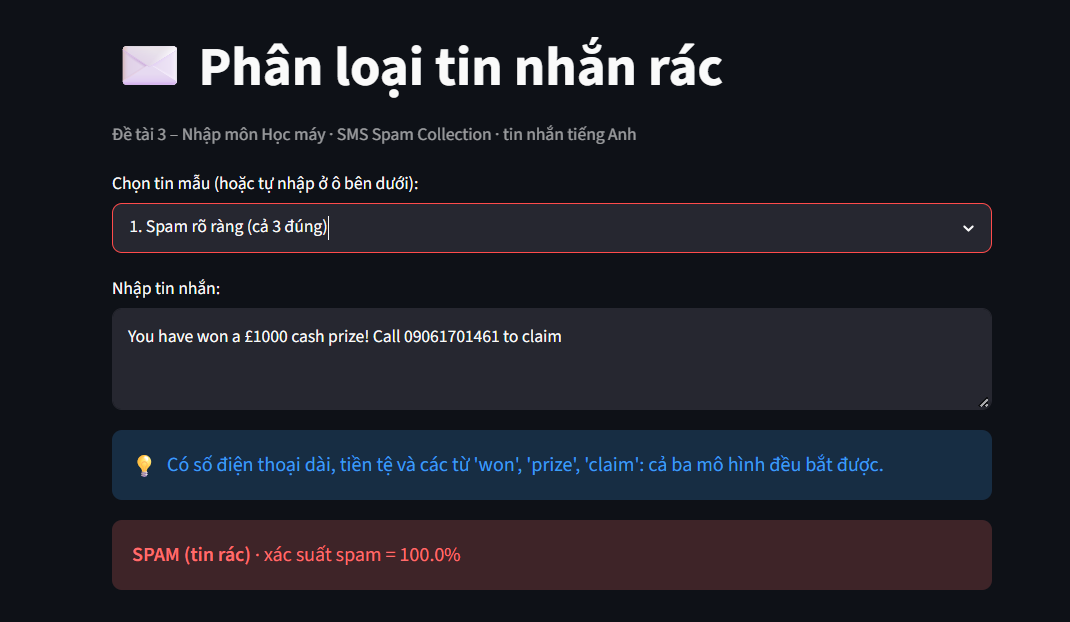
\includegraphics[width=0.92\textwidth]{images/demo_result_spam.png}
    \caption{Hộp cảnh báo màu đỏ rực rỡ khi mô hình phát hiện tin nhắn SPAM}
    \label{fig:demo-result-spam}
\end{figure}

\noindent\textbf{HAM:}
\begin{figure}[H]
    \centering
    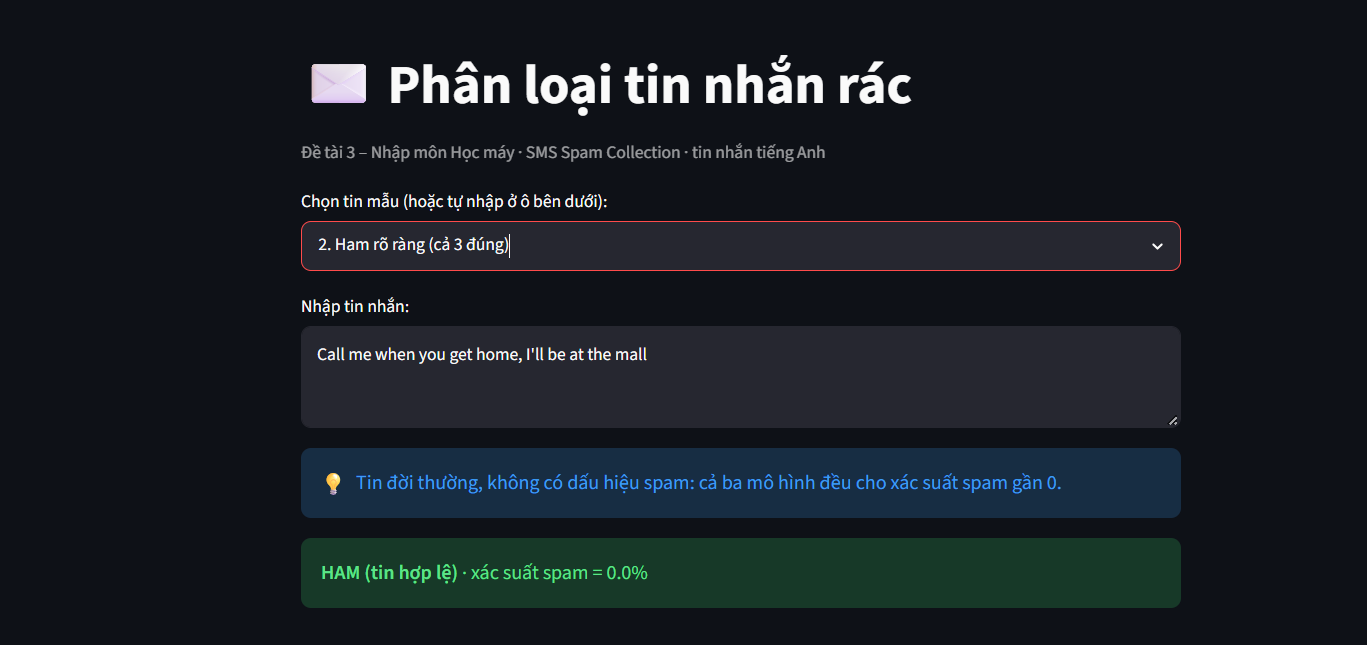
\includegraphics[width=0.92\textwidth]{images/demo_result_ham.png}
    \caption{Hộp thông báo màu xanh lá cây an toàn khi mô hình xác định tin nhắn hợp lệ HAM}
    \label{fig:demo-result-ham}
\end{figure}

\noindent\textbf{*Bảng so sánh 3 mô hình:}
\begin{figure}[H]
    \centering
    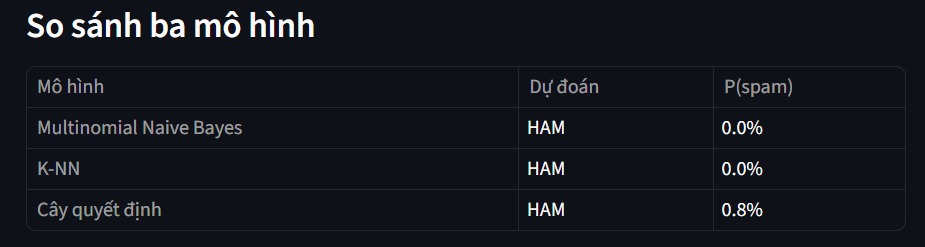
\includegraphics[width=0.85\textwidth]{images/demo_model_comparison.png}
    \caption{Bảng so sánh kết quả dự đoán và xác suất spam của cả ba mô hình trên cùng một tin nhắn}
    \label{fig:demo-model-comparison}
\end{figure}

\subsection{Khối giải thích cơ chế mô hình (Model Explainability Panel)}
Nằm trong một khối đóng mở linh hoạt (\texttt{st.expander}) với tiêu đề *“Mô hình nhìn thấy gì? (tiền xử lý và từ ảnh hưởng)”*:
\begin{enumerate}
    \item \textbf{Hiển thị văn bản sau chuẩn hóa:} Khối mã nguồn hiển thị chuỗi văn bản sau khi đã đi qua hàm \texttt{normalize\_text}. Người dùng có thể quan sát trực tiếp cách các số điện thoại dài bị biến thành \texttt{longnumtoken}, đường dẫn web thành \texttt{urltoken} và ký hiệu tiền tệ thành \texttt{currtoken}.
    \item \textbf{Bảng phân rã đóng góp từ vựng (Feature Contribution Table):}
    Khi mô hình được chọn là Multinomial Naive Bayes, hệ thống trích xuất toàn bộ các từ trong tin nhắn có mặt trong từ điển của mô hình, tính toán mức độ đóng góp theo công thức:
    \begin{equation}
    \text{Contribution}(w_i) = \text{count}(w_i) \times \left[ \ln \hat{P}(w_i | \text{spam}) - \ln \hat{P}(w_i | \text{ham}) \right]
    \end{equation}
    và hiển thị dưới dạng bảng dữ liệu có thể cuộn, sắp xếp từ có giá trị đóng góp dương lớn nhất (kéo mạnh về phía SPAM) đến các từ có giá trị âm lớn nhất (kéo mạnh về phía HAM). Đây là tính năng minh chứng rõ nét cho việc sinh viên làm chủ trọn vẹn bản chất toán học của thuật toán.
\end{enumerate}

\begin{figure}[H]
    \centering
    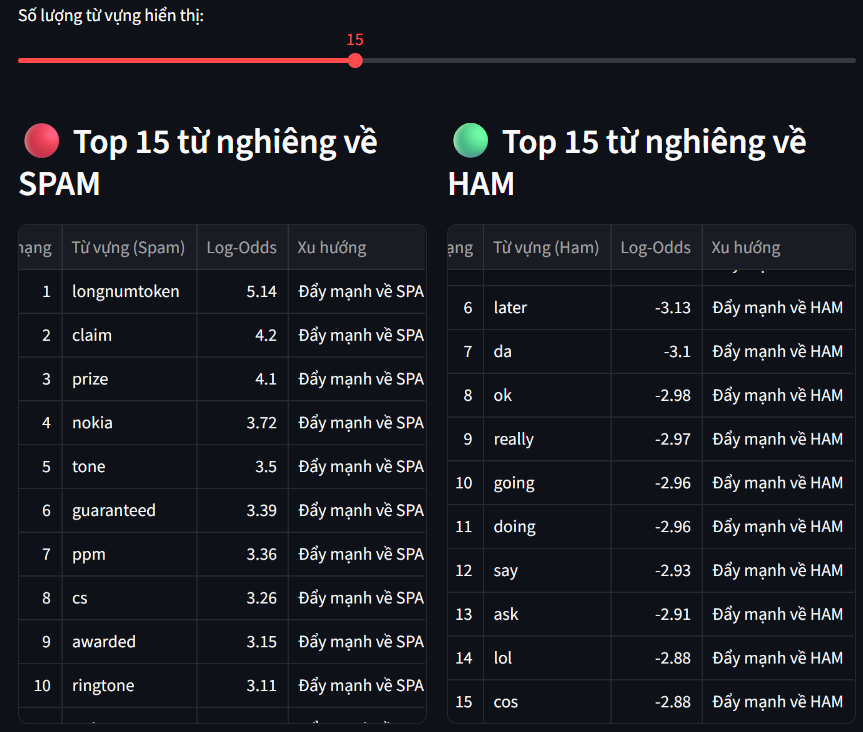
\includegraphics[width=0.95\textwidth]{images/demo_explainability.png}
    \caption{Khối giải thích "Mở hộp đen" với chuỗi tiền xử lý và bảng phân rã đóng góp xác suất Log-Odds}
    \label{fig:demo-explainability}
\end{figure}

\section{Bộ 8 kịch bản kiểm thử mẫu (Demonstration Test Cases)}
\label{sec:8-kich-ban-mau}

Để phục vụ công tác báo cáo và bảo vệ đồ án trước Hội đồng chấm thi một cách thuyết phục nhất, nhóm đã biên soạn một kịch bản trình diễn chuẩn xác gồm 8 tình huống kiểm thử (được lưu trữ tại \texttt{HUONG\_DAN\_DEMO.md}). Các tình huống này được lựa chọn có chủ đích nhằm làm nổi bật cả ưu điểm lẫn các ranh giới bất đồng giữa ba trường phái học máy.

\subsection{Chi tiết 8 kịch bản kiểm thử mẫu}
\begin{enumerate}
    \item \textbf{Tin mẫu 1 --- Spam rõ ràng đầy đủ dấu hiệu (Cả 3 mô hình cùng đúng):}
    \begin{figure}[H]
        \centering
        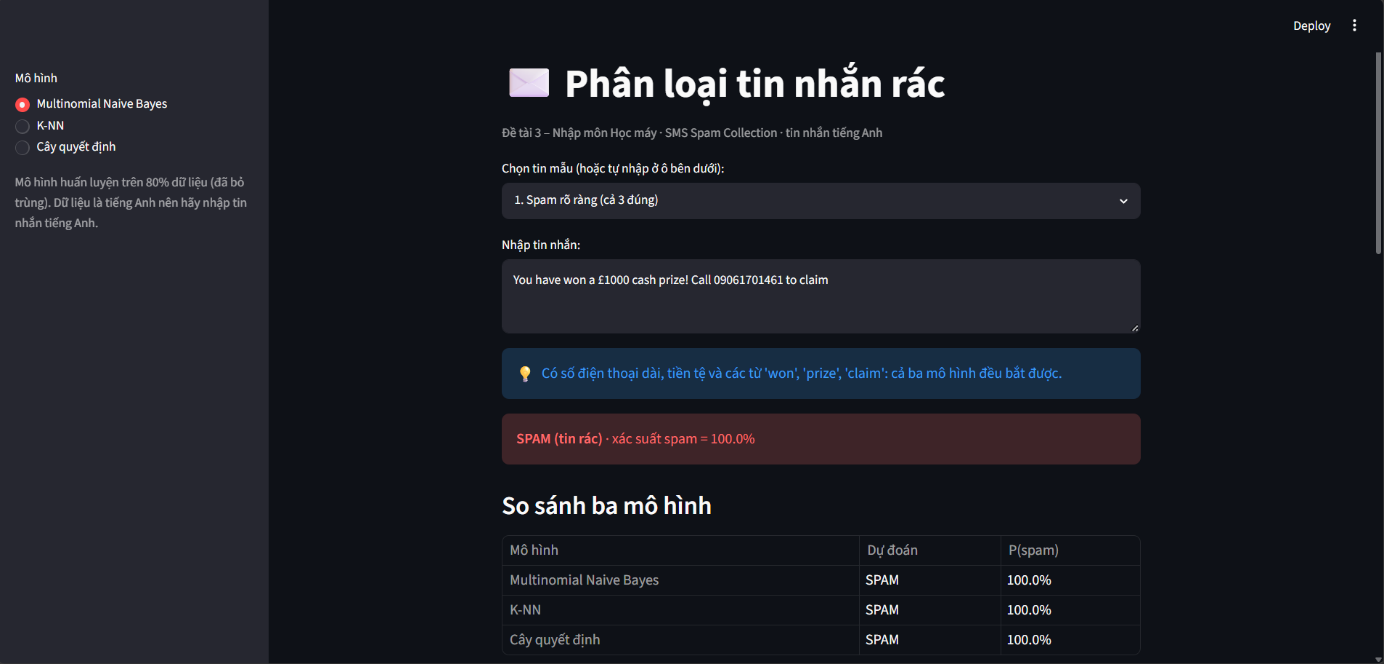
\includegraphics[width=0.92\textwidth]{images/demo_case1.png}
        \caption{Minh chứng thực nghiệm Tin mẫu 1 trên giao diện Demo}
        \label{fig:demo-case1}
    \end{figure}
    \begin{itemize}
        \item \textit{Nội dung:} \texttt{“You have won a £1000 cash prize! Call 09061701461 to claim”}
        \item \textit{Phân tích kỹ thuật:} Tin nhắn chứa đồng thời ký hiệu tiền tệ (£ $\rightarrow$ \texttt{currtoken}), chuỗi số dài (\texttt{longnumtoken}) và các từ khóa đặc trưng (\texttt{won}, \texttt{prize}, \texttt{claim}). Cả ba mô hình đều dự đoán SPAM với xác suất tuyệt đối $100\%$.
    \end{itemize}
    
    \item \textbf{Tin mẫu 2 --- Ham rõ ràng thường nhật (Cả 3 mô hình cùng đúng):}
    \begin{figure}[H]
        \centering
        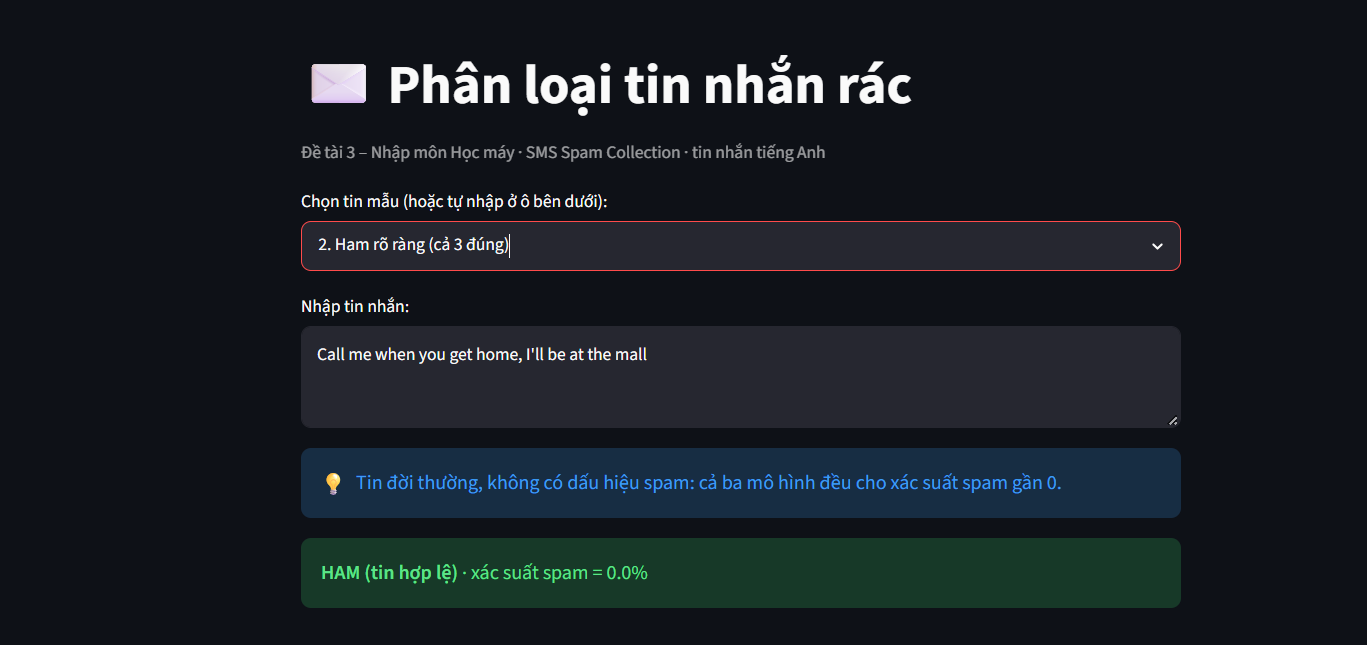
\includegraphics[width=0.92\textwidth]{images/demo_result_ham.png}
        \caption{Minh chứng thực nghiệm Tin mẫu 2 trên giao diện Demo}
        \label{fig:demo-case2}
    \end{figure}
    \begin{itemize}
        \item \textit{Nội dung:} \texttt{“Call me when you get home, I'll be at the mall”}
        \item \textit{Phân tích kỹ thuật:} Tin nhắn giao tiếp gia đình, chứa các từ đời thường (\texttt{call}, \texttt{home}, \texttt{mall}). Cả ba mô hình đều dự đoán HAM với xác suất spam gần bằng $0\%$.
    \end{itemize}
    
    \item \textbf{Tin mẫu 3 --- Ham chứa từ khóa nhạy cảm (Naive Bayes và K-NN báo nhầm; Cây quyết định đúng):}
    \begin{figure}[H]
        \centering
        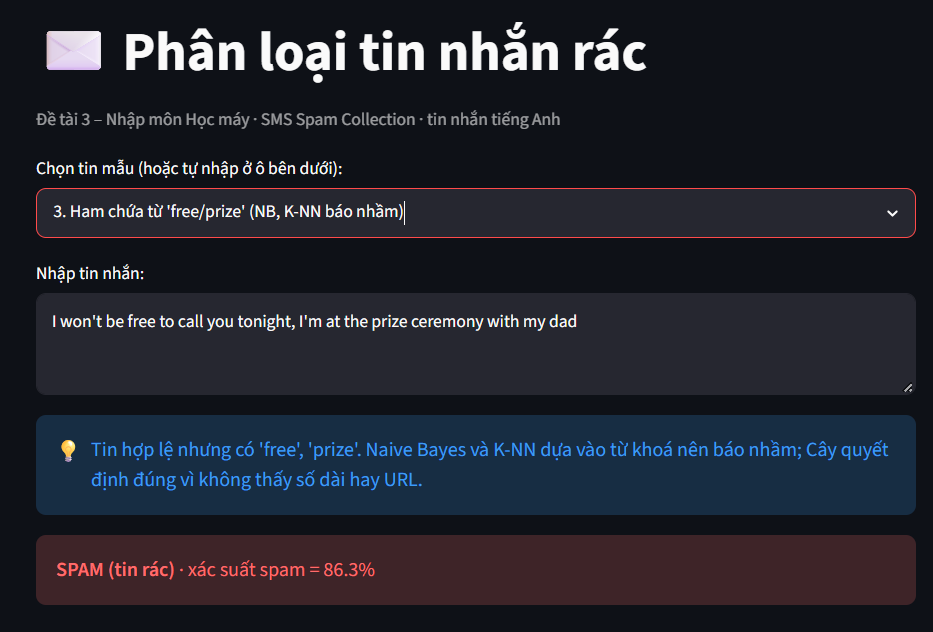
\includegraphics[width=0.92\textwidth]{images/demo_case3.png}
        \caption{Minh chứng thực nghiệm Tin mẫu 3 trên giao diện Demo}
        \label{fig:demo-case3}
    \end{figure}
    \begin{itemize}
        \item \textit{Nội dung:} \texttt{“I won't be free to call you tonight, I'm at the prize ceremony with my dad”}
        \item \textit{Phân tích kỹ thuật:} Tin nhắn hoàn toàn hợp lệ của sinh viên nhắn cho người thân, nhưng có chứa hai từ ngữ nhạy cảm thường thấy trong tin nhắn rác là \texttt{free} và \texttt{prize}. Do Naive Bayes cộng dồn điểm log-odds của từng từ độc lập và K-NN tìm kiếm láng giềng dựa trên trùng lặp từ khóa, cả hai mô hình này đều phát chuông báo động nhầm (Dương tính giả FP). Ngược lại, Cây quyết định dự đoán chính xác là HAM vì cây kiểm tra quy tắc cấu trúc: tin nhắn không chứa số điện thoại dài (\texttt{longnumtoken}) hay đường dẫn web (\texttt{urltoken}).
    \end{itemize}
    
    \item \textbf{Tin mẫu 4 --- Spam chứa liên kết URL (Cây quyết định đúng; K-NN bỏ sót):}
    \begin{figure}[H]
        \centering
        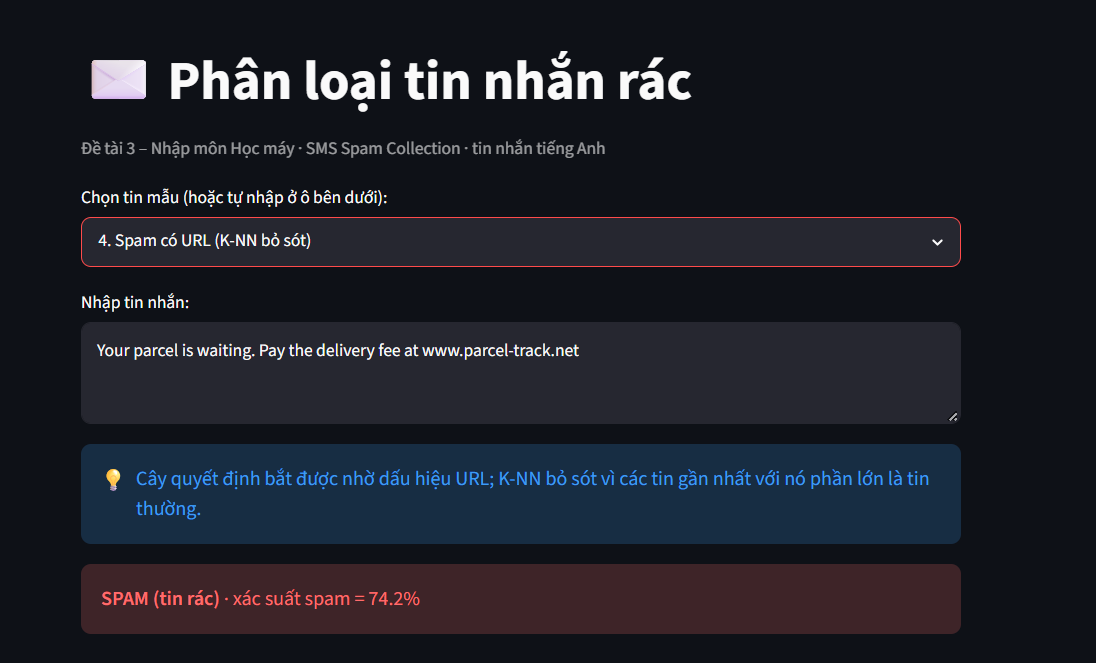
\includegraphics[width=0.92\textwidth]{images/demo_case4.png}
        \caption{Minh chứng thực nghiệm Tin mẫu 4 trên giao diện Demo}
        \label{fig:demo-case4}
    \end{figure}
    \begin{itemize}
        \item \textit{Nội dung:} \texttt{“Your parcel is waiting. Pay the delivery fee at www.parcel-track.net”}
        \item \textit{Phân tích kỹ thuật:} Tin nhắn lừa đảo mạo danh bưu điện phát tán đường dẫn web. Cây quyết định bắt gọn nhờ nhánh kiểm tra \texttt{urltoken}. Tuy nhiên, K-NN bỏ sót (Âm tính giả FN) do các từ đời thường như *“parcel”*, *“waiting”*, *“delivery”* khiến tin nhắn này nằm gần các mẫu tin nhắn hợp lệ trong không gian biểu diễn.
    \end{itemize}
    
    \item \textbf{Tin mẫu 5 --- Spam cuộc gọi nhỡ (Cây quyết định và Naive Bayes đúng; K-NN sát ngưỡng):}
    \begin{figure}[H]
        \centering
        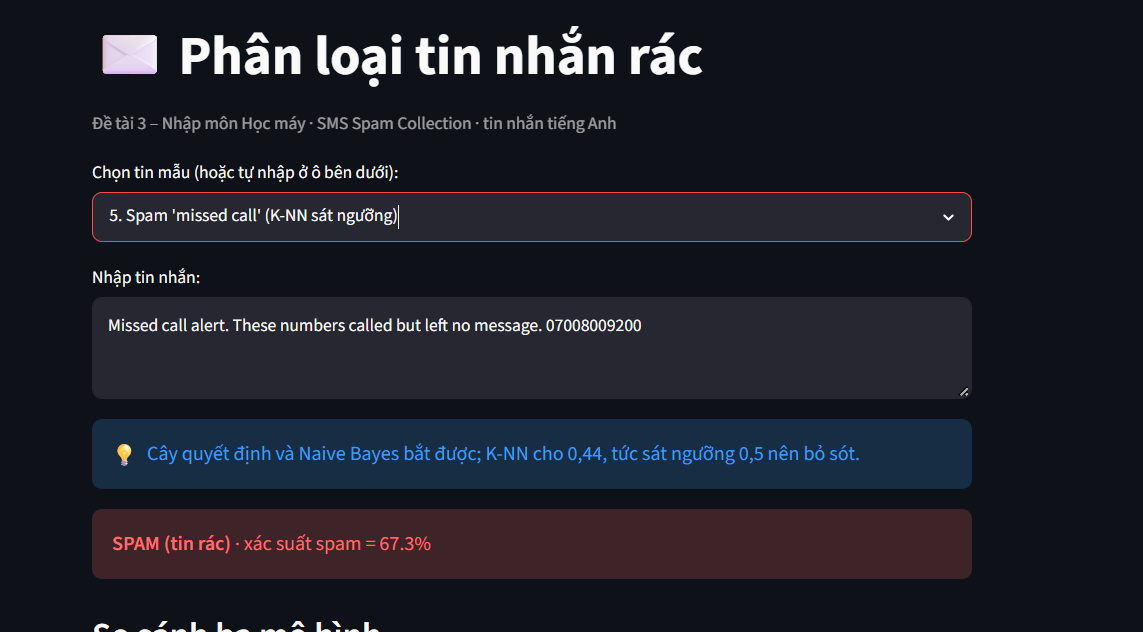
\includegraphics[width=0.92\textwidth]{images/demo_case5.png}
        \caption{Minh chứng thực nghiệm Tin mẫu 5 trên giao diện Demo}
        \label{fig:demo-case5}
    \end{figure}
    \begin{itemize}
        \item \textit{Nội dung:} \texttt{“Missed call alert. These numbers called but left no message. 07008009200”}
        \item \textit{Phân tích kỹ thuật:} Cây quyết định và Naive Bayes bắt chính xác nhờ chuỗi số dài $11$ chữ số (\texttt{longnumtoken}). K-NN tính toán xác suất spam đạt $44\%$, nằm sát ngưỡng phân định $50\%$ nhưng vẫn bị phân loại sót thành ham do biểu quyết đa số.
    \end{itemize}
    
    \item \textbf{Tin mẫu 6 --- Spam không chứa số dài hay URL (Naive Bayes và K-NN đúng; Cây quyết định bỏ sót):}
    \begin{figure}[H]
        \centering
        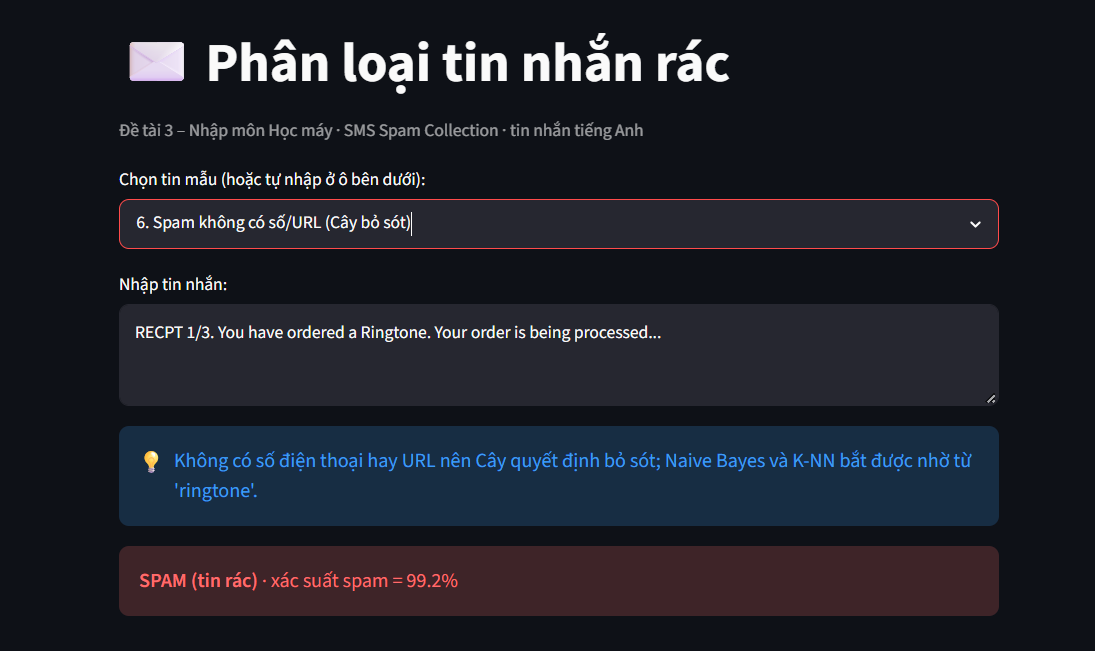
\includegraphics[width=0.92\textwidth]{images/demo_case6.png}
        \caption{Minh chứng thực nghiệm Tin mẫu 6 trên giao diện Demo}
        \label{fig:demo-case6}
    \end{figure}
    \begin{itemize}
        \item \textit{Nội dung:} \texttt{“RECPT 1/3. You have ordered a Ringtone. Your order is being processed...”}
        \item \textit{Phân tích kỹ thuật:} Tin nhắn spam dịch vụ nhạc chuông nhưng không để lại số hotline hay website liên hệ. Cây quyết định bị bỏ sót (FN) do không thỏa mãn luật kiểm tra nút gốc. Ngược lại, Naive Bayes và K-NN nhận diện thành công nhờ trọng số từ vựng tiếp thị mạnh của từ \texttt{ringtone} và \texttt{ordered}.
    \end{itemize}
    
    \item \textbf{Tin mẫu 7 --- Ham ngắn chứa từ thương hiệu (Naive Bayes và K-NN nhầm; Cây quyết định đúng):}
    \begin{figure}[H]
        \centering
        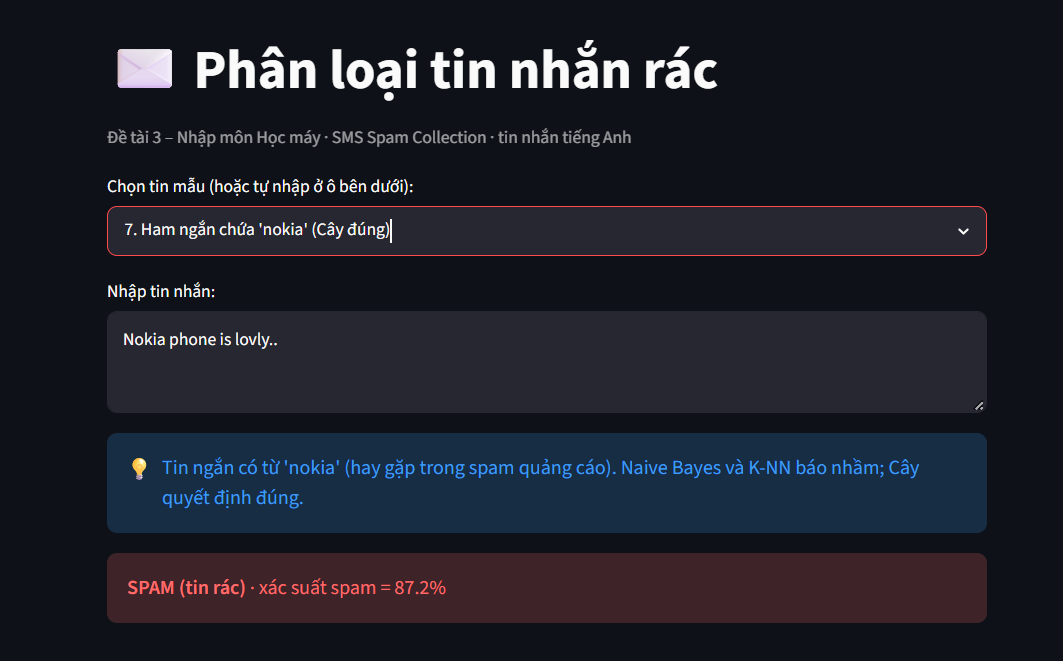
\includegraphics[width=0.92\textwidth]{images/demo_case7.png}
        \caption{Minh chứng thực nghiệm Tin mẫu 7 trên giao diện Demo}
        \label{fig:demo-case7}
    \end{figure}
    \begin{itemize}
        \item \textit{Nội dung:} \texttt{“Nokia phone is lovly..”}
        \item \textit{Phân tích kỹ thuật:} Đây chính là ca Dương tính giả (FP) kinh điển đã mổ xẻ tại Chương 5. Naive Bayes và K-NN bị từ \texttt{nokia} đánh lừa; Cây quyết định giữ vững sự kiên định nhờ không có số dài.
    \end{itemize}
    
    \item \textbf{Tin mẫu 8 --- Spam tinh vi dạng câu đố truyền thông (Cả 3 mô hình cùng sai):}
    \begin{figure}[H]
        \centering
        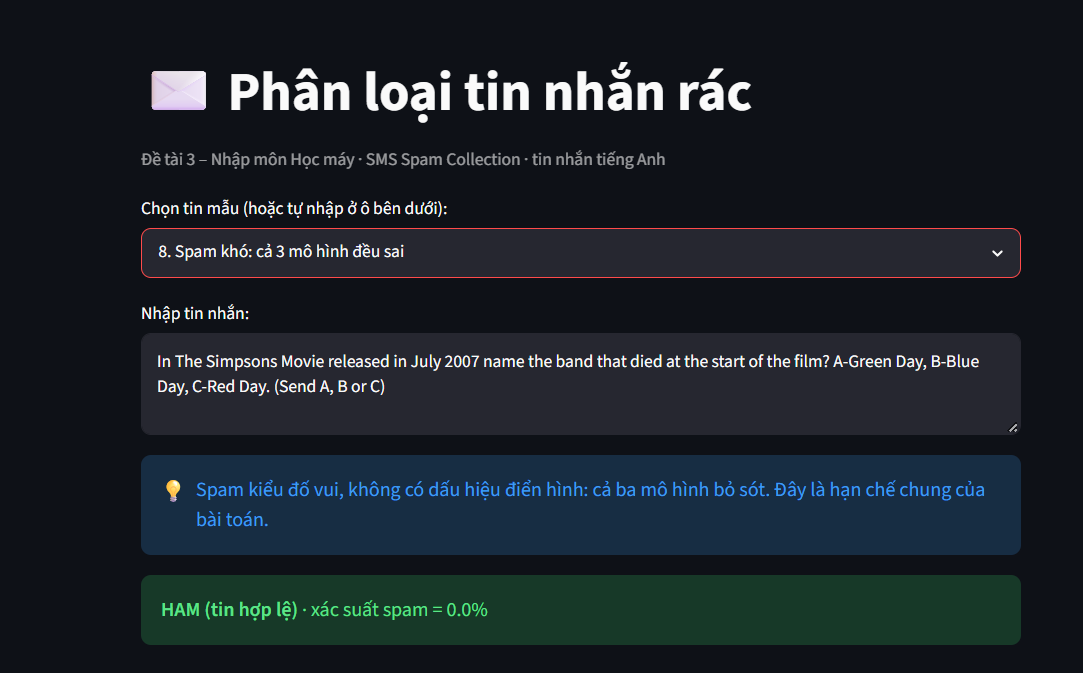
\includegraphics[width=0.92\textwidth]{images/demo_case8.png}
        \caption{Minh chứng thực nghiệm Tin mẫu 8 trên giao diện Demo}
        \label{fig:demo-case8}
    \end{figure}
    \begin{itemize}
        \item \textit{Nội dung:} \texttt{“In The Simpsons Movie released in July 2007 name the band that died at the start of the film? A-Green Day, B-Blue Day, C-Red Day. (Send A, B or C)”}
        \item \textit{Phân tích kỹ thuật:} Ca Âm tính giả (FN) chung của cả ba mô hình. Tin nhắn hoàn toàn thiếu vắng các từ khóa tiếp thị và tín hiệu cấu trúc, minh chứng cho giới hạn tự nhiên của các mô hình học máy dựa trên túi từ BoW và TF-IDF.
    \end{itemize}
\end{enumerate}

\subsection{Kịch bản trình diễn 5 phút trước Hội đồng bảo vệ}
Nhóm đã đúc kết quy trình thuyết trình sản phẩm trực quan gồm 5 bước chặt chẽ:
\begin{itemize}
    \item \textbf{Phút 0:00 -- 0:30:} Mở giao diện Streamlit tại \texttt{localhost:8501}, giới thiệu tổng quan đề tài, quy mô dữ liệu và bài toán phân loại nhị phân mất cân bằng.
    \item \textbf{Phút 0:30 -- 1:15:} Giới thiệu bố cục giao diện, thanh chọn mô hình và bảng đối sánh kết quả ba mô hình song song.
    \item \textbf{Phút 1:15 -- 2:00:} Trình diễn Tin mẫu 1 (Spam rõ) và Tin mẫu 2 (Ham rõ), giải thích rằng với 98,2\% tin nhắn thông thường cả 3 mô hình đều đồng thuận tuyệt đối.
    \item \textbf{Phút 2:00 -- 4:00:} Trình diễn các trường hợp bất đồng kỹ thuật sâu sắc: Tin mẫu 3 (giải thích vì sao Cây quyết định thông minh hơn Naive Bayes khi gặp từ \texttt{free}/\texttt{prize}), Tin mẫu 6 (giải thích vì sao Naive Bayes bắt được \texttt{ringtone} còn Cây bị mù). Mở bảng Log-Odds Attribution để chứng minh cơ chế tính điểm toán học.
    \item \textbf{Phút 4:00 -- 5:00:} Trình diễn Tin mẫu 8 (thừa nhận trung thực hạn chế của mô hình trước spam câu đố) và kết luận về việc lựa chọn mô hình Naive Bayes kết hợp điều chỉnh ngưỡng quyết định trong thực tiễn.
\end{itemize}

\section{Công cụ dòng lệnh CLI (\texttt{src/predict.py})}
\label{sec:cli-predict}

Bên cạnh giao diện web đồ họa Streamlit, nhóm đã phát triển công cụ dòng lệnh độc lập \texttt{src/predict.py} nhằm phục vụ mục đích tự động hóa, kiểm thử hàng loạt (Batch testing) hoặc tích hợp mô hình vào các đường ống xử lý ngầm (Backend daemons/Cron jobs).

\subsection{Phương thức vận hành}
Chương trình tự động nạp mô hình tối ưu đã lưu tại \texttt{results/best\_model.joblib} và vận hành linh hoạt theo hai chế độ:
\begin{enumerate}
    \item \textbf{Chế độ đối số dòng lệnh (Command-line arguments):}
    Truyền trực tiếp một hoặc nhiều chuỗi tin nhắn văn bản vào đối số thực thi:
    
    \begin{figure}[H]
        \centering
        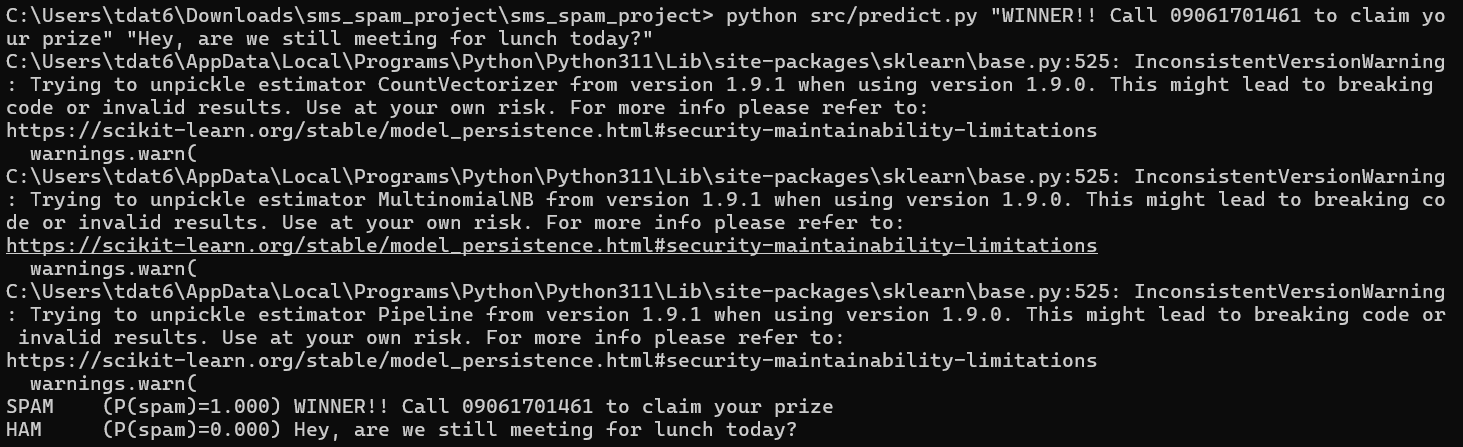
\includegraphics[width=0.95\textwidth]{images/demo_cli_predict.png}
        \caption{Minh chứng thực thi công cụ dòng lệnh CLI src/predict.py trong Terminal}
        \label{fig:demo-cli-predict}
    \end{figure}
    \begin{lstlisting}[language=bash]
python src/predict.py "WINNER!! Call 09061701461 to claim your prize" "Hey, are we still meeting for lunch today?"
    \end{lstlisting}
    Chương trình lập tức trả về kết quả chuẩn hóa dạng tab-separated:
    \begin{lstlisting}[language=bash]
SPAM    (P(spam)=1.000)    WINNER!! Call 09061701461 to claim your prize
HAM     (P(spam)=0.000)    Hey, are we still meeting for lunch today?
    \end{lstlisting}
    
    \item \textbf{Chế độ tương tác nhập liệu liên tục (Interactive shell):}
    Khi chạy lệnh \texttt{python src/predict.py} không kèm đối số, chương trình mở một dấu nhắc lệnh tương tác \texttt{$>$ }, cho phép người dùng gõ liên tục từng tin nhắn và nhận kết quả tức thời, kết thúc bằng một dòng trống.
\end{enumerate}

\section{Tổng kết các kết quả đạt được của đề tài}
\label{sec:tong-ket-ket-qua}

Sau quá trình nghiên cứu lý thuyết, thiết kế hệ thống, thực nghiệm quy mô lớn và phát triển ứng dụng, Nhóm 13 đã hoàn thành xuất sắc toàn bộ các mục tiêu đặt ra với những kết quả nổi bật:
\begin{enumerate}
    \item \textbf{Xây dựng quy trình học máy NLP hoàn chỉnh và chuẩn mực:} Hoàn thiện chu trình khép kín từ tiền xử lý dữ liệu thô, loại bỏ 403 mẫu trùng lặp, chia tách Stratified Train/Test 80/20, đóng gói đường ống \texttt{Pipeline} kiểm soát 100\% nguy cơ rò rỉ dữ liệu (Data Leakage).
    \item \textbf{Sáng tạo kỹ thuật tiền xử lý bảo toàn tín hiệu cấu trúc:} Kỹ thuật quy đổi số dài, URL, tiền tệ thành các token đặc biệt (\texttt{longnumtoken}, \texttt{urltoken}, \texttt{currtoken}) đã chứng minh hiệu quả vượt bậc, đóng góp tới $74,6\%$ tầm quan trọng của Cây quyết định và cải thiện rõ rệt điểm F1 của toàn bộ hệ thống.
    \item \textbf{Thực hiện khối lượng thực nghiệm đồ sộ có tính kiểm soát cao:} Khảo sát toàn diện 36 cấu hình dữ liệu ở Giai đoạn 1; thực hiện tinh chỉnh tối ưu siêu tham số chuyên sâu bằng \texttt{GridSearchCV} 5-fold CV ở Giai đoạn 2; khảo sát mở rộng độ nhạy tham số $\alpha \in [0.1, 10.0]$; phân tích độc lập tác động của n-gram, \texttt{min\_df}, \texttt{max\_df} và giới hạn \texttt{max\_features}.
    \item \textbf{Khẳng định mô hình tối ưu toàn diện:} Xác lập \textbf{Multinomial Naive Bayes} ($\alpha=2.0$, P2, BoW unigram) là mô hình dẫn đầu với F1-score kiểm thử đạt \textbf{$0,9653$}, Recall \textbf{$95,42\%$}, Accuracy \textbf{$99,13\%$}, tốc độ dự đoán cực nhanh $27.900$ tin/giây và duy trì độ ổn định cao nhất qua 5 seed ngẫu nhiên ($F_1 = 0,9467 \pm 0,0195$).
    \item \textbf{Khám phá các phát hiện khoa học và cạm bẫy dữ liệu sâu sắc:} Chỉ ra sai lầm phương pháp luận khi đánh giá TF-IDF trên tham số mặc định $\alpha=1.0$; giải thích thất bại của khoảng cách Euclid trên K-NN; vạch trần cạm bẫy dữ liệu HTML \texttt{lt}/\texttt{gt} sinh ra từ quá trình ẩn danh hóa số điện thoại.
    \item \textbf{Phát triển ứng dụng Demo và CLI hoàn thiện:} Xây dựng thành công ứng dụng web Streamlit trực quan, hỗ trợ so sánh đa mô hình, bộ 8 kịch bản kiểm thử mẫu và cơ chế giải thích quyết định XAI minh bạch.
\end{enumerate}

\section{Hướng nghiên cứu và phát triển mở rộng trong tương lai}
\label{sec:huong-phat-trien}

Mặc dù hệ thống đã đạt được hiệu năng rất cao trên bộ ngữ liệu thực nghiệm, để tiến tới triển khai một giải pháp lọc tin nhắn thương mại thực thụ trong môi trường viễn thông thực tế, nhóm đề xuất một số hướng nghiên cứu và phát triển mở rộng:
\begin{enumerate}
    \item \textbf{Tối ưu hóa ngưỡng cắt quyết định (Decision Threshold Tuning):}
    Trong hệ thống hiện tại, ngưỡng phân loại xác suất mặc định là $\tau = 0.5$. Trong môi trường vận hành thực tế nơi chi phí của lỗi Dương tính giả (FP) là cực kỳ đắt, có thể dịch chuyển ngưỡng quyết định lên mức khắt khe hơn (ví dụ $\tau = 0.8$ hoặc $\tau = 0.9$) hoặc tối ưu hóa ngưỡng dựa trên đường cong Precision-Recall nhằm triệt tiêu hoàn toàn nguy cơ chặn nhầm tin nhắn quan trọng của khách hàng.
    \item \textbf{Mở rộng ngữ liệu và thích ứng đa ngôn ngữ (Tiếng Việt):}
    Thu thập và gán nhãn tập ngữ liệu tin nhắn rác tiếng Việt hiện đại, tích hợp các công cụ tách từ tiếng Việt chuyên biệt (như \texttt{pyvi}, \texttt{underthesea}) và bổ sung các mẫu tin nhắn lừa đảo tài chính thế hệ mới (mạo danh biến động số dư ngân hàng, bẫy đầu tư tài chính, lừa đảo việc làm online).
    \item \textbf{Ứng dụng các mô hình học sâu và biểu diễn ngữ nghĩa tiên tiến (Deep Learning \& Transformers):}
    Thử nghiệm các kiến trúc n-gram ký tự (Character-level n-grams) để chống lại thủ đoạn cố tình viết sai chính tả (ví dụ: *“cl4im pr1ze”*), kết hợp các mô hình ngôn ngữ tiền huấn luyện tiên tiến (như BERT, RoBERTa hoặc PhoBERT cho tiếng Việt) để nắm bắt sâu sắc ngữ cảnh toàn cục của câu văn.
    \item \textbf{Đóng gói vi dịch vụ (Microservices Containerization) và Triển khai Đám mây:}
    Đóng gói toàn bộ hệ thống phân loại thành các Docker container chuẩn hóa, xây dựng giao diện lập trình ứng dụng RESTful API bằng FastAPI, và tích hợp cơ chế lắng nghe phản hồi của người dùng (User Feedback Loop) để liên tục tái huấn luyện mô hình (Online Active Learning).
\end{enumerate}

\section{Tóm tắt chương 6}
Chương 6 đã khép lại công trình nghiên cứu bằng việc giới thiệu trọn vẹn sản phẩm ứng dụng demo tương tác Streamlit và công cụ dòng lệnh CLI. Hệ thống cung cấp khả năng phân loại tức thời, đối sánh đa mô hình trực quan và giải thích quyết định dựa trên đóng góp log-odds của từng từ vựng. Bộ 8 kịch bản kiểm thử mẫu được thiết kế công phu đã làm nổi bật các sắc thái kỹ thuật đa dạng giữa ba trường phái học máy. Chương này cũng đã tổng kết toàn diện các đóng góp nổi bật của đề tài và vạch ra lộ trình phát triển rõ ràng để nâng cấp hệ thống thành một giải pháp an ninh viễn thông thương mại vững chắc.

% =========================
% PHẦN CUỐI BÁO CÁO
% =========================
\clearpage
\UnnumberedChapter{KẾT LUẬN}

Quá trình triển khai và hoàn thiện Bài tập lớn học phần \textbf{Nhập môn Học máy (mã học phần: FIT4013)} với Đề tài 3: \textit{“Phân loại tin nhắn rác (SMS Spam Collection) --- Nghiên cứu so sánh các thuật toán Multinomial Naive Bayes, K-NN và Cây quyết định”} đã mang lại cho tập thể Nhóm 13 những trải nghiệm học tập và nghiên cứu khoa học vô cùng quý giá, sâu sắc và toàn diện.

Vượt lên trên khuôn khổ của việc sao chép một đoạn mã nguồn mẫu hay thực thi một cuốn sổ tay Jupyter đơn lẻ, nhóm đã xây dựng thành công một quy trình phân tích dữ liệu và học máy khép kín, chuẩn mực và có tính tái lập tuyệt đối. Từ 5.574 tin nhắn thô ban đầu, nhóm đã khám phá và phân tích sâu sắc các đặc trưng hình thái, cấu trúc và phân phối xác suất; nhận diện và xử lý triệt để 403 bản ghi trùng lặp nhằm xóa bỏ hoàn toàn rủi ro rò rỉ dữ liệu; sáng tạo kỹ thuật tiền xử lý bảo toàn tín hiệu thông qua các token đại diện chuyên biệt; thiết kế không gian thực nghiệm đa chiều gồm 36 cấu hình dữ liệu và đóng gói khép kín trong \texttt{sklearn.pipeline.Pipeline}.

Kết quả thực nghiệm đã đem lại những phát hiện có giá trị phương pháp luận sâu sắc:
\begin{enumerate}
    \item Khẳng định mô hình \textbf{Multinomial Naive Bayes} ($\alpha=2.0$, tiền xử lý P2, biểu diễn BoW unigram) là giải pháp tối ưu toàn diện nhất cho bài toán phân loại tin nhắn rác SMS, đạt F1-score kiểm thử lên tới \textbf{$0,9653$}, Recall \textbf{$95,42\%$}, Accuracy \textbf{$99,13\%$}, tốc độ dự đoán vượt trội $27.900$ tin nhắn/giây và duy trì độ ổn định cao nhất qua 5 seed ngẫu nhiên ($F_1 = 0,9467 \pm 0,0195$).
    \item Làm sáng tỏ hiện tượng suy giảm hiệu năng của TF-IDF trên Naive Bayes ở tham số mặc định $\alpha=1.0$, chứng minh rằng khi được tinh chỉnh siêu tham số phù hợp theo từng ô cấu hình, TF-IDF và BoW mang lại hiệu năng tương đương nhau.
    \item Chứng minh bản chất thất bại của khoảng cách Euclid trên thuật toán K-NN khi áp dụng cho dữ liệu văn bản thưa, và chứng minh bước nhảy vọt của K-NN khi kết hợp vector hóa TF-IDF với khoảng cách Cosine (F1 tăng từ $0,4217$ lên $0,9291$, đạt ROC-AUC cao nhất toàn hệ thống $0,9919$).
    \item Xác nhận tính chất đặc thù của Cây quyết định với khả năng diễn giải luật tường minh và đạt chỉ số Precision tuyệt đối $100\%$ nhờ sự chi phối của đặc trưng chuỗi số dài \texttt{longnumtoken} (chiếm $74,6\%$ tầm quan trọng của cây).
    \item Mổ xẻ chi tiết 9 ca dự đoán sai của Naive Bayes (3 FP và 6 FN), nhận diện các điểm mù của mô hình trước các tin nhắn ngắn mang tính thương mại hoặc tin nhắn spam thiếu vắng tín hiệu cấu trúc, đồng thời phát hiện cạm bẫy dữ liệu HTML \texttt{lt}/\texttt{gt} sinh ra từ quá trình ẩn danh hóa số điện thoại.
    \item Hiện thực hóa trọn vẹn sản phẩm ứng dụng web tương tác thời gian thực bằng Streamlit và công cụ dòng lệnh CLI, tích hợp bộ 8 kịch bản kiểm thử mẫu và cơ chế giải thích quyết định dựa trên đóng góp log-odds của từng từ vựng.
\end{enumerate}

Bên cạnh những kết quả học thuật và kỹ thuật đã đạt được, bài tập lớn đã giúp từng thành viên trong nhóm rèn luyện và trưởng thành vượt bậc về các kỹ năng cốt lõi: tư duy phân tích dữ liệu phản biện, kỹ năng lập trình hướng pipeline tái lập, kỹ năng thiết kế thực nghiệm có đối chứng, kỹ năng làm việc nhóm và phối hợp quản lý mã nguồn bằng GitHub, cũng như kỹ năng biên soạn báo cáo khoa học chuẩn mực bằng hệ thống soạn thảo chuyên nghiệp \LaTeX.

Nhóm xin chân thành cảm ơn sự hướng dẫn tận tình, tâm huyết của giảng viên ThS. Lê Thị Thùy Trang. Những kiến thức và phương pháp luận tiếp thu được từ học phần này chắc chắn sẽ là bệ phóng vững chắc cho các công trình nghiên cứu chuyên sâu, đồ án tốt nghiệp và sự nghiệp kỹ sư công nghệ thông tin tương lai của mỗi thành viên trong nhóm.

\clearpage
\UnnumberedChapter{DANH MỤC TÀI LIỆU THAM KHẢO}

\section*{Tiếng Việt}

\begin{enumerate}[label={[\arabic*]}]
    \item Lê Thị Thùy Trang. (2026). \textit{Bài giảng học phần Nhập môn Học máy (FIT4013): Bài 1 đến Bài 6}. Khoa Công nghệ Thông tin, Trường Đại học Đại Nam.
    \item Lê Thị Thùy Trang. (2026). \textit{Hướng dẫn thực hiện bài tập lớn học phần Nhập môn Học máy (FIT4013) --- Năm học 2026--2027}. Khoa Công nghệ Thông tin, Trường Đại học Đại Nam.
    \item Vũ Hữu Tiệp. (2018). \textit{Machine Learning cơ bản}. NXB Khoa học và Kỹ thuật, Hà Nội.
    \item Lương Chi Mai \& ctg. (2015). \textit{Giáo trình Xử lý Ngôn ngữ Tự nhiên}. NXB Đại học Quốc gia Hà Nội, Hà Nội.
    \item Nguyễn Thị Hoàng Lan. (2020). \textit{Các phương pháp khai phá văn bản và ứng dụng}. NXB Thông tin và Truyền thông, Hà Nội.
\end{enumerate}

\section*{Tiếng Anh}

\begin{enumerate}[label={[\arabic*]}, resume]
    \item Almeida, T. A., Gómez Hidalgo, J. M., \& Yamakami, A. (2011). Contributions to the study of SMS spam filtering: new collection and results. In \textit{Proceedings of the 11th ACM Symposium on Document Engineering (DocEng '11)}, pp. 259--262. ACM, Mountain View, California, USA. DOI: \url{https://doi.org/10.1145/2022409.2022461}.
    \item Almeida, T. A., \& Gómez Hidalgo, J. M. (2011). \textit{SMS Spam Collection v.1}. UCI Machine Learning Repository. DOI: \url{https://doi.org/10.24432/C5CC84}. Giấy phép Creative Commons Attribution 4.0 International (CC BY 4.0).
    \item Müller, A. C., \& Guido, S. (2016). \textit{Introduction to Machine Learning with Python: A Guide for Data Scientists}. O'Reilly Media, Sebastopol, CA.
    \item Pedregosa, F., Varoquaux, G., Gramfort, A., Michel, V., Thirion, B., Grisel, O., Blondel, M., Prettenhofer, P., Weiss, R., Dubourg, V., Vanderplas, J., Passos, A., Cournapeau, D., Brucher, M., Perrot, M., \& Duchesnay, E. (2011). Scikit-learn: Machine Learning in Python. \textit{Journal of Machine Learning Research}, 12, pp. 2825--2830.
    \item Hastie, T., Tibshirani, R., \& Friedman, J. (2009). \textit{The Elements of Statistical Learning: Data Mining, Inference, and Prediction} (2nd ed.). Springer-Verlag, New York.
    \item Jurafsky, D., \& Martin, J. H. (2024). \textit{Speech and Language Processing: An Introduction to Natural Language Processing, Computational Linguistics, and Speech Recognition} (3rd ed. draft). Prentice Hall.
    \item Manning, C. D., Raghavan, P., \& Schütze, H. (2008). \textit{Introduction to Information Retrieval}. Cambridge University Press, Cambridge, UK.
    \item Géron, A. (2022). \textit{Hands-On Machine Learning with Scikit-Learn, Keras, and TensorFlow: Concepts, Tools, and Techniques to Build Intelligent Systems} (3rd ed.). O'Reilly Media.
    \item Fawcett, T. (2006). An introduction to ROC analysis. \textit{Pattern Recognition Letters}, 27(8), pp. 861--874.
    \item McCallum, A., \& Nigam, K. (1998). A comparison of event models for Naive Bayes text classification. In \textit{AAAI-98 Workshop on Learning for Text Categorization}, Vol. 752, pp. 41--48.
\end{enumerate}

\clearpage
\appendix
\UnnumberedChapter{PHỤ LỤC}

\section*{Phụ lục A. Báo cáo khai báo sử dụng công cụ Trí tuệ Nhân tạo (AI)}
\addcontentsline{toc}{section}{Phụ lục A. Báo cáo khai báo sử dụng công cụ Trí tuệ Nhân tạo (AI)}

Căn cứ theo quy định tại Mục 2.3 và Tiêu chí Liêm chính học thuật trong Rubric đánh giá bài tập lớn tại Mục 2.5 của tài liệu \textit{“Hướng dẫn thực hiện bài tập lớn học phần Nhập môn Học máy (FIT4013) --- ThS. Lê Thị Thùy Trang”}, tập thể Nhóm 13 xin khai báo công khai, minh bạch toàn bộ quá trình sử dụng các công cụ Trí tuệ nhân tạo (AI) trong quá trình triển khai đề tài như sau:

\subsection*{1. Các công cụ AI đã sử dụng}
\begin{itemize}
    \item \textbf{Claude 3.5 Sonnet / Claude 3.7 Sonnet (Anthropic):} Sử dụng thông qua giao diện hội thoại lập trình và trợ lý mã nguồn.
    \item \textbf{Antigravity / Gemini Pro (Google DeepMind):} Sử dụng hỗ trợ tra cứu tài liệu học thuật, gợi ý cấu trúc báo cáo khoa học và rà soát cú pháp \LaTeX.
\end{itemize}

\subsection*{2. Các nội dung và nhiệm vụ được AI hỗ trợ}
\begin{enumerate}
    \item \textbf{Khảo sát và đối chiếu yêu cầu môn học:} Hỗ trợ đọc hiểu tài liệu hướng dẫn bài tập lớn và toàn bộ 6 bài giảng của học phần FIT4013, từ đó đề xuất thiết kế quy trình thực nghiệm tuân thủ chặt chẽ yêu cầu của Đề tài 3.
    \item \textbf{Gợi ý kiến trúc đường ống học máy (Pipeline):} Đề xuất cấu trúc mã nguồn hướng module hóa trong thư mục \texttt{src/}, tư vấn việc đóng gói vectorizer và mô hình bên trong \texttt{sklearn.pipeline.Pipeline} để ngăn ngừa rò rỉ dữ liệu (Data Leakage).
    \item \textbf{Phát hiện và tháo gỡ lỗi kỹ thuật trong dữ liệu:}
    \begin{itemize}
        \item Phát hiện lỗi phân tách dòng trong tệp \texttt{SMSSpamCollection} do chứa ký tự dấu nháy kép (\texttt{"}) và ký hiệu tiền tệ Anh (£) làm mất một số dòng khi đọc bằng cấu hình mặc định của \texttt{pandas}; gợi ý giải pháp sử dụng tham số \texttt{quoting=csv.QUOTE\_NONE}.
        \item Cảnh báo rủi ro rò rỉ dữ liệu của 403 tin nhắn trùng lặp, đề xuất phương án loại bỏ trùng lặp trước khi phân chia train/test.
        \item Phát hiện cạm bẫy phương pháp luận: chỉ ra việc so sánh biểu diễn BoW và TF-IDF với siêu tham số mặc định $\alpha=1.0$ là không công bằng đối với Naive Bayes, gợi ý chuyển đổi sang quy trình tinh chỉnh siêu tham số theo từng ô cấu hình ở Giai đoạn 2.
    \end{itemize}
    \item \textbf{Hỗ trợ rà soát cú pháp \LaTeX:} Chuyển đổi các bảng kết quả định lượng từ định dạng CSV sang bảng mã nguồn \LaTeX\ chuẩn mực, hỗ trợ căn chỉnh lề, định dạng tiêu đề và kiểm tra liên kết chéo.
\end{enumerate}

\subsection*{3. Phần công việc nhóm tự thực hiện, kiểm chứng và chịu trách nhiệm}
\begin{itemize}
    \item Nhóm trực tiếp cài đặt môi trường, chạy toàn bộ các kịch bản thực nghiệm trên máy tính cá nhân, kiểm chứng từng con số trong các tệp CSV và JSON sinh ra từ mã nguồn.
    \item Nhóm tự tay kiểm tra từng tin nhắn dự đoán sai trong tập phân tích lỗi, đối chiếu nguyên nhân ngôn ngữ học và xác thực tính đúng đắn của các giải thích.
    \item Nhóm kiểm tra, chạy thử và hoàn thiện toàn bộ giao diện ứng dụng web Streamlit và kịch bản demo 8 tin mẫu.
    \item \textbf{Cam kết liêm chính học thuật:} Toàn bộ các thành viên trong nhóm hiểu rõ bản chất toán học, cấu trúc mã nguồn, quy trình đường ống và kết quả thực nghiệm của đề tài; sẵn sàng thuyết minh, phản biện và trả lời độc lập mọi câu hỏi chuyên môn của Hội đồng chấm thi khi bảo vệ bài tập lớn.
\end{itemize}

\clearpage

\section*{Phụ lục B. Bảng phân công nhiệm vụ và minh chứng đóng góp nhóm}
\addcontentsline{toc}{section}{Phụ lục B. Bảng phân công nhiệm vụ và minh chứng đóng góp nhóm}

Nhóm 13 gồm 02 thành viên thuộc lớp CNTT 18-10, Khoa Công nghệ Thông tin, Trường Đại học Đại Nam. Quá trình làm việc nhóm được điều phối thông qua kho lưu trữ mã nguồn GitHub tại địa chỉ: \url{https://github.com/hhai258/NMHM-CNTT-1810-NHOM-13}.

Bảng~\ref{tab:phan-cong-nhiem-vu} tổng hợp chi tiết phần việc phụ trách, nhiệm vụ kỹ thuật và tỷ lệ đóng góp của từng thành viên:

\begin{table}[H]
\centering
\caption{Bảng phân công nhiệm vụ và tỷ lệ hoàn thành công việc của Nhóm 13}
\label{tab:phan-cong-nhiem-vu}
\begin{tabular}{|c|p{4cm}|c|p{6.5cm}|c|}
\hline
\textbf{STT} & \textbf{Họ và tên thành viên} & \textbf{Mã sinh viên} & \textbf{Nhiệm vụ chính phụ trách} & \textbf{Tỷ lệ đóng góp} \\
\hline
\textbf{1} & \textbf{Nguyễn Hoàng Hải} (Trưởng nhóm) & 1871020211 &
\begin{itemize}[leftmargin=*, nosep]
    \item Khám phá và phân tích dữ liệu (EDA).
    \item Xây dựng module tiền xử lý dữ liệu và hàm chuẩn hóa regex \texttt{normalize\_text}.
    \item Thiết kế cấu trúc \texttt{Pipeline} và thực nghiệm Giai đoạn 1 (36 cấu hình).
    \item Thực nghiệm tối ưu hóa siêu tham số GridSearchCV (Giai đoạn 2).
    \item Viết báo cáo các Chương 1, 2, 3 và Phụ lục A, C.
\end{itemize}
& \textbf{50\%} \\
\hline
\textbf{2} & \textbf{Nguyễn Thành Đạt} & 1871020135 &
\begin{itemize}[leftmargin=*, nosep]
    \item Thực nghiệm mở rộng độ nhạy tham số làm trơn $\alpha$ cho Naive Bayes.
    \item Thực nghiệm có kiểm soát về tham số Vectorizer (\texttt{vectorizer\_sensitivity.py}).
    \item Đánh giá trên tập test, ma trận nhầm lẫn và kiểm tra độ ổn định 5-seed.
    \item Phân tích lỗi chi tiết (FP, FN) và trích xuất độ quan trọng Log-Odds.
    \item Phát triển ứng dụng web demo Streamlit và viết Chương 4, 5, 6.
\end{itemize}
& \textbf{50\%} \\
\hline
\end{tabular}
\Nguon{Nhóm 13 thống nhất và lập biên bản phân công}
\end{table}

\clearpage

\section*{Phụ lục C. Hướng dẫn cài đặt môi trường và tái lập thực nghiệm}
\addcontentsline{toc}{section}{Phụ lục C. Hướng dẫn cài đặt môi trường và tái lập thực nghiệm}

Để tái lập toàn bộ quy trình nghiên cứu từ dữ liệu thô đến kết quả cuối cùng, người dùng có thể thực hiện theo các bước tuần tự dưới đây trên môi trường dòng lệnh (Command Prompt hoặc PowerShell):

\subsection*{1. Tải mã nguồn từ GitHub và khởi tạo môi trường ảo}
\begin{lstlisting}[language=bash]
# 1. Clone repository ve may cuc bo
git clone https://github.com/hhai258/NMHM-CNTT-1810-NHOM-13.git
cd NMHM-CNTT-1810-NHOM-13

# 2. Tao va kich hoat moi truong ao Python
python -m venv .venv
# Tren Windows:
.venv\Scripts\activate
# Tren Linux / macOS:
source .venv/bin/activate

# 3. Cai dat cac thu vien khoa hoc du lieu
pip install -r requirements.txt
\end{lstlisting}

\subsection*{2. Chạy tái lập toàn bộ chuỗi thực nghiệm}
\begin{lstlisting}[language=bash]
# 1. Chay thuc nghiem chinh (EDA -> GridSearch -> Test -> Error Analysis)
# Thoi gian chay: khoang 8 - 10 phut tren CPU 1 loi
python src/run_experiments.py

# 2. (Tuy chon) Chay kiem tra do nhay he so alpha mo rong
python src/extra_nb_alpha_check.py

# 3. (Tuy chon) Chay thuc nghiem do nhay cac tham so Vectorizer
python src/vectorizer_sensitivity.py
\end{lstlisting}

\subsection*{3. Chạy thử nghiệm phân loại nhanh qua giao diện dòng lệnh (CLI)}
\begin{lstlisting}[language=bash]
# Du doan mot chuoi tin nhan cu the:
python src/predict.py "WINNER!! Call 09061701461 to claim your prize"

# Hoac chay o che do nhap lieu tuong tac truc tiep:
python src/predict.py
\end{lstlisting}

\subsection*{4. Khởi chạy ứng dụng giao diện web demo Streamlit}
\begin{lstlisting}[language=bash]
# 1. Cai dat goi streamlit (neu chua co)
pip install -r requirements-demo.txt

# 2. Khoi dong ung dung web
streamlit run src/demo_app.py
\end{lstlisting}
Trình duyệt web sẽ tự động mở trang tương tác tại địa chỉ: \url{http://localhost:8501}.

\clearpage

\section*{Phụ lục D. Trích đoạn mã nguồn các hàm xử lý cốt lõi}
\addcontentsline{toc}{section}{Phụ lục D. Trích đoạn mã nguồn các hàm xử lý cốt lõi}

\subsection*{1. Hàm chuẩn hóa văn bản bảo toàn tín hiệu (\texttt{src/common.py})}
\begin{lstlisting}[language=Python]
def normalize_text(s: str) -> str:
    """Chuan hoa giu tin hieu: thay the URL, so dai, tien te bang token dac biet."""
    s = s.lower()
    s = URL_RE.sub(" urltoken ", s)
    s = CURR_RE.sub(" currtoken ", s)
    s = LONGNUM_RE.sub(" longnumtoken ", s)
    s = NUM_RE.sub(" numtoken ", s)
    s = re.sub(r"[^a-z\s]", " ", s)           # Loai bo dau cau con lai
    return re.sub(r"\s+", " ", s).strip()
\end{lstlisting}

\subsection*{2. Hàm khởi tạo Vectorizer và đóng gói Pipeline (\texttt{src/common.py})}
\begin{lstlisting}[language=Python]
def make_vectorizer(prep_name, rep_name):
    p, r = PREPROCESS[prep_name], REPRESENT[rep_name]
    cls = CountVectorizer if r["kind"] == "bow" else TfidfVectorizer
    kw = dict(lowercase=True, ngram_range=r["ngram_range"], min_df=r["min_df"],
              stop_words=p["stop_words"])
    if p["preprocessor"] is not None:
        kw["preprocessor"] = p["preprocessor"]
    return cls(**kw)

def make_pipeline(model_name, prep_name, rep_name, model=None, memory=None):
    """Vectorizer nam TRONG pipeline => chi fit tren tap huan luyen
    (va tren tung fold khi cross-validation) -> tranh data leakage."""
    return Pipeline([("vec", make_vectorizer(prep_name, rep_name)),
                     ("clf", model if model is not None else make_model(model_name))],
                    memory=memory)
\end{lstlisting}

\subsection*{3. Trích đoạn tính toán đóng góp Log-Odds trong Demo App (\texttt{src/demo\_app.py})}
\begin{lstlisting}[language=Python]
if model_key == "MultinomialNB":
    vec, clf = pipe.named_steps["vec"], pipe.named_steps["clf"]
    X = vec.transform([text])
    idx = X.nonzero()[1]
    if len(idx):
        names = vec.get_feature_names_out()
        lo = clf.feature_log_prob_[1] - clf.feature_log_prob_[0]
        contrib = np.asarray(X[0, idx].todense()).ravel() * lo[idx]
        df_c = pd.DataFrame({"Tu vung": names[idx], "Dong gop (log-odds)": contrib.round(2)})
        df_c = df_c.sort_values("Dong gop (log-odds)", ascending=False)
        st.write("Tu day ve **SPAM** (duong) hoac **HAM** (am):")
        st.dataframe(df_c, hide_index=True)
\end{lstlisting}

\end{document}